\documentclass[12pt]{article}

% Packages
\usepackage{amsmath, amssymb, amsthm}
\usepackage{mathtools}
\usepackage{graphicx}
\usepackage{booktabs}
\usepackage{algorithm}
\usepackage{algorithmic}
\usepackage{hyperref}
\usepackage{natbib}
\usepackage{xcolor}
\usepackage{bm}
\usepackage{multirow}
\usepackage{subcaption}
\usepackage{float}
\usepackage{tikz}
\usetikzlibrary{decorations.pathreplacing}
\definecolor{ffblock}{gray}{0.85}   % light grey: function-function
\definecolor{fdblock}{gray}{0.60}   % medium grey: function-derivative
\definecolor{ddblock}{gray}{0.50}   % dark grey: derivative-derivative
\definecolor{ffblock}{RGB}{210, 230, 255}  % light blue: function-function
\definecolor{fdblock}{RGB}{255, 220, 180}  % light orange: function-derivative
\definecolor{ddblock}{RGB}{200, 240, 200}  % light green: derivative-derivative
\definecolor{fhblock}{RGB}{220, 200, 255}   % lavender: function-hessian
\definecolor{ghblock}{RGB}{255, 200, 200}   % light pink: gradient-hessian
\definecolor{hhblock}{RGB}{255, 255, 180}   % light yellow: hessian-hessian
% Page layout
\usepackage[margin=1in]{geometry}

% Math operators
\DeclareMathOperator*{\argmin}{argmin}
\DeclareMathOperator*{\argmax}{argmax}
\DeclareMathOperator{\Cov}{Cov}
\DeclareMathOperator{\Var}{Var}
\DeclareMathOperator{\tr}{tr}

% Theorem environments
\newtheorem{theorem}{Theorem}
\newtheorem{lemma}[theorem]{Lemma}
\newtheorem{proposition}[theorem]{Proposition}
\newtheorem{corollary}[theorem]{Corollary}
\newtheorem{remark}{Remark}
\newtheorem{definition}{Definition}

% Custom commands
\newcommand{\R}{\mathbb{R}}
\newcommand{\N}{\mathbb{N}}
\newcommand{\E}{\mathbb{E}}
\newcommand{\x}{\mathbf{x}}
\newcommand{\y}{\mathbf{y}}
\newcommand{\X}{\mathbf{X}}
\newcommand{\V}{\mathbf{V}}
\newcommand{\vv}{\mathbf{v}}
\newcommand{\balpha}{\boldsymbol{\alpha}}
\newcommand{\bbeta}{\boldsymbol{\beta}}
\newcommand{\bgamma}{\boldsymbol{\gamma}}
\newcommand{\bpsi}{\boldsymbol{\psi}}
\newcommand{\bSigma}{\boldsymbol{\Sigma}}
\newcommand{\bmu}{\boldsymbol{\mu}}

% For editorial notes during drafting
\newcommand{\todo}[1]{\textcolor{red}{[TODO: #1]}}
\newcommand{\note}[1]{\textcolor{blue}{[NOTE: #1]}}

\title{Arbitrary-Order Derivative-Enhanced Gaussian Processes: A Unified Framework with Directional Derivatives and Weighted Decomposition}

\author{
	Samuel Roberts$^{1}$, Mauricio Aristizabal$^{2}$, Juan C. Velasquez-Gonzalez$^{3}$,\\
	David Yamil Risk-Mora$^{1}$, David Restrepo$^{1}$, Harry Millwater$^{1}$\\[1em]
	$^{1}$Department of Mechanical Engineering, University of Texas at San Antonio\\
	$^{2}$Department of Mechanical Engineering, St. Mary's University\\
	$^{3}$Southwest Research Institute
}

\date{\today}

\begin{document}
	
	\maketitle
	
\begin{abstract}
	Derivative-enhanced Gaussian Processes (DEGPs) improve surrogate model accuracy by incorporating gradient and curvature information, but existing methods are limited to at most second-order derivatives and scale poorly with input dimension. This work presents a unified framework for arbitrary-order derivative-enhanced Gaussian Processes that addresses these limitations through three complementary strategies. The Derivative-Enhanced Gaussian Process (DEGP) extends classical gradient-enhanced Gaussian processes to derivatives of any order $p$, with selective derivative screening to manage the combinatorial growth of terms. The Directional Derivative Gaussian Process (DDGP) achieves dimension-independent computational complexity by using derivatives along $q \ll d$ selected directions rather than all $d$ coordinate directions. The Weighted Derivative-Enhanced Gaussian Process (WDEGP) extends weighted gradient-enhanced Gaussian processes to arbitrary order.
	\vspace{1em}
	\noindent\textbf{Keywords:} Gaussian Processes, Derivative-Enhanced Gaussian Processes, Directional Derivatives, Surrogate Modeling, Uncertainty Quantification
\end{abstract}


	
	\newpage
	\tableofcontents
	\newpage
	
	%==============================================================================
	\section*{Nomenclature}
	\label{sec:nomenclature}
	%==============================================================================
	
	\subsection*{General Notation}
	\begin{tabular}{@{}l l@{}}
		$d$ & Dimension of input space \\
		$n$ & Number of training points \\
		$n_*$ & Number of test points \\
		$p$ & Maximum derivative order \\
		$q$ & Number of directional derivative directions \\
		$M$ & Number of submodels (WDEGP/WDDGP) \\
		$\mathbf{x}, \mathbf{x}_i$ & Input vector, $i$-th training input \\
		$\mathbf{X}$ & Training input matrix, $\{\mathbf{x}_i\}_{i=1}^{n}$ \\
		$\mathbf{X}_*$ & Test input matrix \\
		$f(\mathbf{x})$ & Function value at $\mathbf{x}$ \\
		$\mathbf{y}$ & Observation vector \\
	\end{tabular}
	
	\subsection*{Kernel and Hyperparameters}
	\begin{tabular}{@{}l l@{}}
		$k(\mathbf{x}, \mathbf{x}')$ & Kernel (covariance) function \\
		$K(\mathbf{X}, \mathbf{X}')$ & Kernel matrix with entries $[K]_{ij} = k(\mathbf{x}_i, \mathbf{x}_j)$ \\
		$\boldsymbol{\psi}$ & Kernel hyperparameters \\
		$\sigma_f^2$ & Signal variance \\
		$\boldsymbol{\theta}$ & Length scale parameters \\
		$\sigma_n^2$ & Noise variance \\
	\end{tabular}
	
	\subsection*{Covariance Block Notation}
	\begin{tabular}{@{}l l@{}}
		$\boldsymbol{\Sigma}_{11}$ & Training-training covariance block \\
		$\boldsymbol{\Sigma}_{12}$ & Training-test covariance block \\
		$\boldsymbol{\Sigma}_{21}$ & Test-training covariance block ($= \boldsymbol{\Sigma}_{12}^\top$) \\
		$\boldsymbol{\Sigma}_{22}$ & Test-test covariance block \\
		$\boldsymbol{\mu}_*$ & Posterior predictive mean \\
		$\boldsymbol{\Sigma}_*$ & Posterior predictive covariance \\
	\end{tabular}
	
	\subsection*{Derivative Notation}
	\begin{tabular}{@{}l l@{}}
		$\boldsymbol{\alpha} = (\alpha_1, \ldots, \alpha_d)$ & Multi-index for partial derivatives \\
		$|\boldsymbol{\alpha}| = \sum_{j=1}^{d} \alpha_j$ & Total order of multi-index $\boldsymbol{\alpha}$ \\
		$D^{\boldsymbol{\alpha}} f$ & Partial derivative: $\partial^{|\boldsymbol{\alpha}|}_{x_1^{\alpha_1} \cdots x_d^{\alpha_d}} f$ \\
		$\boldsymbol{\beta} = (\beta_1, \ldots, \beta_q)$ & Multi-index for directional derivatives \\
		$D_{\mathbf{V}}^{\boldsymbol{\beta}} f$ & Directional derivative: $\partial^{|\boldsymbol{\beta}|}_{\mathbf{v}_1^{\beta_1} \cdots \mathbf{v}_q^{\beta_q}} f$ \\
		$\partial^n_{(\cdot)} K$ & Compact notation for $n$-th order kernel derivatives (see Section~\ref{subsec:derivative_gps}) \\
		$\mathbf{v}, \mathbf{v}_{i,j}$ & Direction vector, $j$-th direction at point $i$ \\
		$\mathbf{V}_i$ & Set of direction vectors at training point $i$ \\
		$\mathbf{V}$ & Collection of all training direction vectors $\{\mathbf{v}_{i,j}\}$ \\
		$\mathbf{V}_*$ & Collection of all test direction vectors $\{\mathbf{v}_{*i,j}\}$ \\
	\end{tabular}
	
	\subsection*{Index Sets}
	\begin{tabular}{@{}l l@{}}
		$\mathcal{A}_p$ & Complete set of partial derivative multi-indices up to order $p$ \\
		& $\mathcal{A}_p = \{\boldsymbol{\alpha} \in \mathbb{N}_0^d : |\boldsymbol{\alpha}| \leq p\}$, with $|\mathcal{A}_p| = \binom{d+p}{p}$ \\
		$\mathcal{A}_{\text{sel}}$ & Selected subset of partial derivative multi-indices \\
		$\mathcal{B}_p^q$ & Complete set of directional derivative multi-indices up to order $p$ \\
		& $\mathcal{B}_p^q = \{\boldsymbol{\beta} \in \mathbb{N}_0^q : |\boldsymbol{\beta}| \leq p\}$, with $|\mathcal{B}_p^q| = \binom{q+p}{q}$ \\
		$\mathcal{B}_{\text{sel}}$ & Selected subset of directional derivative multi-indices \\
		$\mathcal{I}_g$ & Index set of training points with gradient observations \\
		$n_g$ & Number of gradient-observed training points ($|\mathcal{I}_g|$) \\
		$\mathbf{X}_g$ & Gradient-observed training locations $\{\mathbf{x}_i \mid i \in \mathcal{I}_g\}$ \\
		$\mathcal{I}_k$ & Training point indices assigned to submodel $k$ \\
	\end{tabular}
	
	\subsection*{Superscripts and Subscripts}
	\begin{tabular}{@{}l l@{}}
		$(\cdot)^{(k)}$ & Quantity associated with submodel $k$ \\
		$(\cdot)^{\text{scr}}$ & Screened (reduced) quantity \\
		$(\cdot)^{R}$ & Reduced gradient-enhanced quantity \\
		$(\cdot)^{DD}$ & Directional derivative quantity \\
		$(\cdot)^{G}$ & Gradient-enhanced quantity \\
		$(\cdot)^{H}$ & Hessian-enhanced quantity \\
		$M_{\text{sel}}$ & Number of selected partial derivative terms \\
		$L_{\text{sel}}$ & Number of selected directional derivative terms \\
		$N_k^{\text{deriv}}$ & Number of derivative observations in submodel $k$ \\
	\end{tabular}
	
	\subsection*{Abbreviations}
	\begin{tabular}{@{}l l@{}}
		GP & Gaussian Process \\
		DEGP & Derivative-Enhanced Gaussian Process \\
		DDGP & Directional Derivative Gaussian Process \\
		WDEGP & Weighted Derivative-Enhanced Gaussian Process \\
		WDDGP & Weighted Directional Derivative Gaussian Process \\
		GEGP & Gradient-Enhanced Gaussian Process \\
		HEGP & Hessian-Enhanced Gaussian Process \\
		PGEGP & Partial Gradient-Enhanced Gaussian Process \\
		WGEGP & Weighted Gradient-Enhanced Gaussian Process \\
		MLL & Marginal Log-Likelihood \\
		JLL & Joint Log-Likelihood \\
	\end{tabular}
	
	%==============================================================================
	\section{Introduction}
	\label{sec:introduction}
	%==============================================================================
	

	
	%==============================================================================
	\section{Background}
	\label{sec:background}
	%==============================================================================
	

Gaussian Processes (GPs), also referred to as Kriging models in the geostatistics literature, have become one of the most commonly used surrogate modeling techniques in many engineering design applications due to their ability to deliver both predictions and uncertainty estimates \cite{10.1115/DETC2019-97499,georges1963principles, Krig,GP}. They are a non-parametric supervised learning method used to solve regression, optimization, and probabilistic classification problems \cite{rasmussen2006gaussian}. In particular, a Gaussian process can be viewed as a collection of random variables, any finite number of which have a joint Gaussian distribution. A Gaussian Process model can be completely determined by its mean function $m(\mathbf{x})$ and covariance function $k(\mathbf{x}, \mathbf{x}')$ of a real process $f(\mathbf{x})$ as given below:

\begin{equation}
	\label{eqn2}
	\begin{aligned}
		m(\mathbf{x}) &= \mathbb{E}[f(\mathbf{x})], \\
		k(\mathbf{x}, \mathbf{x}') &= \mathbb{E}[(f(\mathbf{x}) - m(\mathbf{x}))(f(\mathbf{x}') - m(\mathbf{x}'))]
	\end{aligned}
\end{equation}

The Gaussian Process can then be written as:

\begin{equation}
	\label{eqn3}
	f(\mathbf{x}) \sim \mathcal{GP}(m(\mathbf{x}), k(\mathbf{x}, \mathbf{x}'))
\end{equation}

The covariance function in \eqref{eqn2} is often approximated by a kernel function which assigns a specific covariance between pairs of random variables so that $\text{cov}\left(f(\mathbf{x}), f(\mathbf{x}')\right) = k(\mathbf{x}, \mathbf{x}')$. The kernel function can take on various forms, one of the most commonly used functions, the squared exponential, is given below:

\begin{equation}
	\label{eqn4}
	K_{SE}(\mathbf{x}, \mathbf{x}', \sigma_f^2, \boldsymbol{\theta}) = \sigma_f^2 \exp\left(-\sum\limits_{i = 1}^{d} \frac{(x_i - x'_i)^2}{2 \theta_i^2} \right)
\end{equation}

In this function, the parameters $\sigma_f^2$ and $\boldsymbol{\theta}$ collectively denoted as $\boldsymbol{\psi} = \{\sigma_f^2, \boldsymbol{\theta}\}$ are the hyperparameters of the model, which are learned from the data:

\begin{itemize}
	\item $\sigma_f^2$ is the \textbf{variance}, which is a scaling factor that controls the overall vertical variation of the function.
	\item $\theta_i$ is the \textbf{length scale} for each input dimension $i$. It determines how quickly the correlation between points decreases with distance. A small length scale means the function varies rapidly, while a large length scale indicates a smoother function.
\end{itemize}

To make predictions using a Gaussian process model, an observed training dataset $\mathcal{D}$ containing $n$ input-output pairs is assumed as given by equation \eqref{data_set}:

\begin{equation}
	\label{data_set}
	\mathcal{D} = \left\{\mathbf{X}, \mathbf{Y} \right\}  = \left\{(\mathbf{x}_i, y_i) \mid i = 1, \ldots, n \right\}
\end{equation}

where each input $\mathbf{x}_i \in \mathbb{R}^d$ has a corresponding observed output $y_i = f(\mathbf{x}_i)$. For now, it is assumed the output of $f$ is scalar, though this framework can be generalized to vector outputs \cite{LIU2018102,Lin2022-rs}.

To predict outputs at a new set of test locations, $\mathbf{X}_*$, the joint distribution over the training and test outputs is modeled. It is common to assume a zero-mean function for the GP, such that $m(\mathbf{x}) = 0$. This assumption simplifies the model but is not overly restrictive, as it only constrains the prior distribution; the posterior predictive mean will be non-zero and adapt to the data. With these assumptions, the joint distribution of the training outputs $\mathbf{y} = f(\mathbf{X})$ and the test outputs $\mathbf{y}_* = f(\mathbf{X}_*)$ is given by:

\begin{equation}
	\label{eqn_joint_dist}
	\begin{pmatrix}
		\mathbf{y} \\
		\mathbf{y}_*
	\end{pmatrix}
	\sim \mathcal{N}\left(
	\begin{pmatrix}
		\mathbf{0} \\
		\mathbf{0}
	\end{pmatrix},
	\begin{pmatrix}
		K(\mathbf{X}, \mathbf{X}') & K(\mathbf{X}, \mathbf{X}_*) \\
		K(\mathbf{X}_*, \mathbf{X}) & K(\mathbf{X}_*, \mathbf{X}_*')
	\end{pmatrix}
	\right)
\end{equation}

Here, the prime notation is a notational convenience: $\mathbf{X}'$ represents the same set of training points as $\mathbf{X}$, but as the second argument of the covariance function. Thus $K(\mathbf{X}, \mathbf{X}')$ evaluates the kernel between all pairs of training points, producing an $n \times n$ covariance matrix with entries $[K(\mathbf{X}, \mathbf{X}')]_{ij} = k(\mathbf{x}_i, \mathbf{x}_j)$. For notational simplicity, this covariance matrix is partitioned into blocks:

\begin{equation}
	\label{eqn_cov_blocks}
	\begin{pmatrix}
		\boldsymbol{\Sigma}_{11} & \boldsymbol{\Sigma}_{12} \\
		\boldsymbol{\Sigma}_{21} & \boldsymbol{\Sigma}_{22}
	\end{pmatrix}
	=
	\begin{pmatrix}
		K(\mathbf{X}, \mathbf{X}') & K(\mathbf{X}, \mathbf{X}_*) \\
		K(\mathbf{X}_*, \mathbf{X}) & K(\mathbf{X}_*, \mathbf{X}_*')
	\end{pmatrix}
\end{equation}

where $\boldsymbol{\Sigma}_{11}$ is the covariance of training points with themselves, $\boldsymbol{\Sigma}_{12}$ is the covariance of training points with test points, $\boldsymbol{\Sigma}_{22}$ is the covariance of the test points with themselves, and $\boldsymbol{\Sigma}_{21} = \boldsymbol{\Sigma}_{12}^T$.

From the multivariate Gaussian theorem, the conditional distribution of a Gaussian is itself Gaussian. This fact allows for making predictions at the test points $\mathbf{X}_*$ conditioned on the training data $\mathcal{D}$. Using the block matrix notation defined in \eqref{eqn_cov_blocks}, the posterior predictive distribution is given by:

\begin{equation}
	\label{eqn_gp_posterior_block}
	\begin{aligned}
		p(\mathbf{y}_* \mid \mathbf{y}) &= \mathcal{N}(\boldsymbol{\mu}_{*}, \boldsymbol{\Sigma}_{*}) \\
		\boldsymbol{\mu}_{*} &= \boldsymbol{\Sigma}_{21} \boldsymbol{\Sigma}_{11}^{-1} \mathbf{y} \\
		\boldsymbol{\Sigma}_{*} &=  \boldsymbol{\Sigma}_{22} - \boldsymbol{\Sigma}_{21} \boldsymbol{\Sigma}_{11}^{-1} \boldsymbol{\Sigma}_{12}
	\end{aligned}
\end{equation}

Here, $\boldsymbol{\mu}_{*}$ is the posterior predictive mean and $\boldsymbol{\Sigma}_{*}$ is the posterior predictive covariance.

The kernel hyperparameters, $\boldsymbol{\psi}$, are not set manually but are instead learned from the training data $\mathcal{D}$. A standard approach is to find the values that maximize the log marginal likelihood of the observations, $p(\mathbf{y} \mid \mathbf{X}, \boldsymbol{\psi})$ \cite{rasmussen2006gaussian}. For a noise-free model, the log marginal likelihood is given by:

\begin{equation}
	\label{MLL}
	\log p(\mathbf{y}|\mathbf{X}, \boldsymbol{\psi}) = -\frac{1}{2} \mathbf{y}^\top \mathbf{K}_{\boldsymbol{\psi}}^{-1} \mathbf{y} - \frac{1}{2}\log|\mathbf{K}_{\boldsymbol{\psi}}| - \frac{n}{2}\log 2\pi
\end{equation}

where $\mathbf{K}_{\boldsymbol{\psi}} = K(\mathbf{X},\mathbf{X})$. Optimized hyperparameters, $\boldsymbol{\psi}^*$, are then selected according to:

\begin{equation}
	\label{maxMLL}
	\boldsymbol{\psi}^* = \argmax_{\boldsymbol{\psi}} \left( \log p(\mathbf{y}|\mathbf{X}, \boldsymbol{\psi}) \right)
\end{equation}

Note that directly computing the expression in \eqref{MLL} requires evaluating both the inverse and determinant of the matrix $K = k(\mathbf{X}, \mathbf{X}')$, operations that are computationally expensive and numerically unstable for large $n$. To address these challenges, the Cholesky decomposition is typically employed \cite{rasmussen2006gaussian}. For a symmetric positive definite matrix $K$, the Cholesky decomposition yields a lower triangular matrix $L$ such that $K = LL^\top$. This factorization enables efficient computation of both the matrix inverse and the log-determinant. Indeed, the Cholesky method is approximately twice as fast as Gaussian elimination for symmetric positive definite matrices \cite{Allaire2008-by}, and it provides better numerical stability, especially for large-scale problems where the kernel matrix may be ill-conditioned.

\subsubsection{Derivative Predictions from a Standard GP}
\label{subsec:gp_deriv_pred}

A key property of Gaussian processes is their closure under linear operators: if $f \sim \mathcal{GP}(m, k)$, then any linear operation $\mathcal{L}[f]$ is also a Gaussian process~\cite{rasmussen2006gaussian}. In particular, the partial derivative $\partial_{x_i} f$ is itself a GP with covariance given by the corresponding derivative of the kernel:
\begin{equation}
	\label{eqn:gp_deriv_cov}
	\mathrm{cov}\!\left[\partial_{x_i} f(\mathbf{x}),\; \partial_{x_j'} f(\mathbf{x}')\right] = \partial^2_{x_i\, x_j'}\, k(\mathbf{x}, \mathbf{x}').
\end{equation}
The cross-covariance between function values and derivatives follows similarly:
\begin{equation}
	\label{eqn:gp_cross_cov}
	\mathrm{cov}\!\left[f(\mathbf{x}),\; \partial_{x_j'} f(\mathbf{x}')\right] = \partial_{x_j'}\, k(\mathbf{x}, \mathbf{x}').
\end{equation}
This means that even when only function values are observed during training, one can form a joint distribution over function values and derivatives at test locations, and condition on the training data to obtain derivative predictions. That is, the test vector $\mathbf{y}_*$ in~\eqref{eqn_joint_dist} is replaced with:
\begin{equation}
	\label{eqn:gp_aug_test}
	\tilde{\mathbf{y}}_* = \begin{bmatrix} f(\mathbf{X}_*) \\ \partial_{x_1} f(\mathbf{X}_*) \\ \vdots \\ \partial_{x_d} f(\mathbf{X}_*) \end{bmatrix},
\end{equation}
while the training vector $\mathbf{y}$ remains unchanged (function values only). The cross-covariance block $\boldsymbol{\Sigma}_{12}$ and test covariance block $\boldsymbol{\Sigma}_{22}$ are augmented with the appropriate kernel derivatives from \eqref{eqn:gp_deriv_cov}--\eqref{eqn:gp_cross_cov}, and the standard posterior equations~\eqref{eqn_gp_posterior_block} apply directly. This produces derivative predictions that are consistent with the learned function, though their accuracy is limited by the absence of derivative training data.

\paragraph{Numerical example.}
To illustrate this, consider a standard GP applied to the test function $f(x_1, x_2) = \sin(x_1)\cos(x_2)$ on $[0, 2\pi]^2$. The model is trained on function values at a $5 \times 5$ grid of $n = 25$ points using a squared exponential kernel. Figure~\ref{fig:gp_example} shows the resulting predictions: the function is interpolated well at the training locations, and derivative predictions capture the correct qualitative structure, but with substantially higher error than the derivative-enhanced methods developed in the following sections.

\begin{figure}[H]
	\centering
	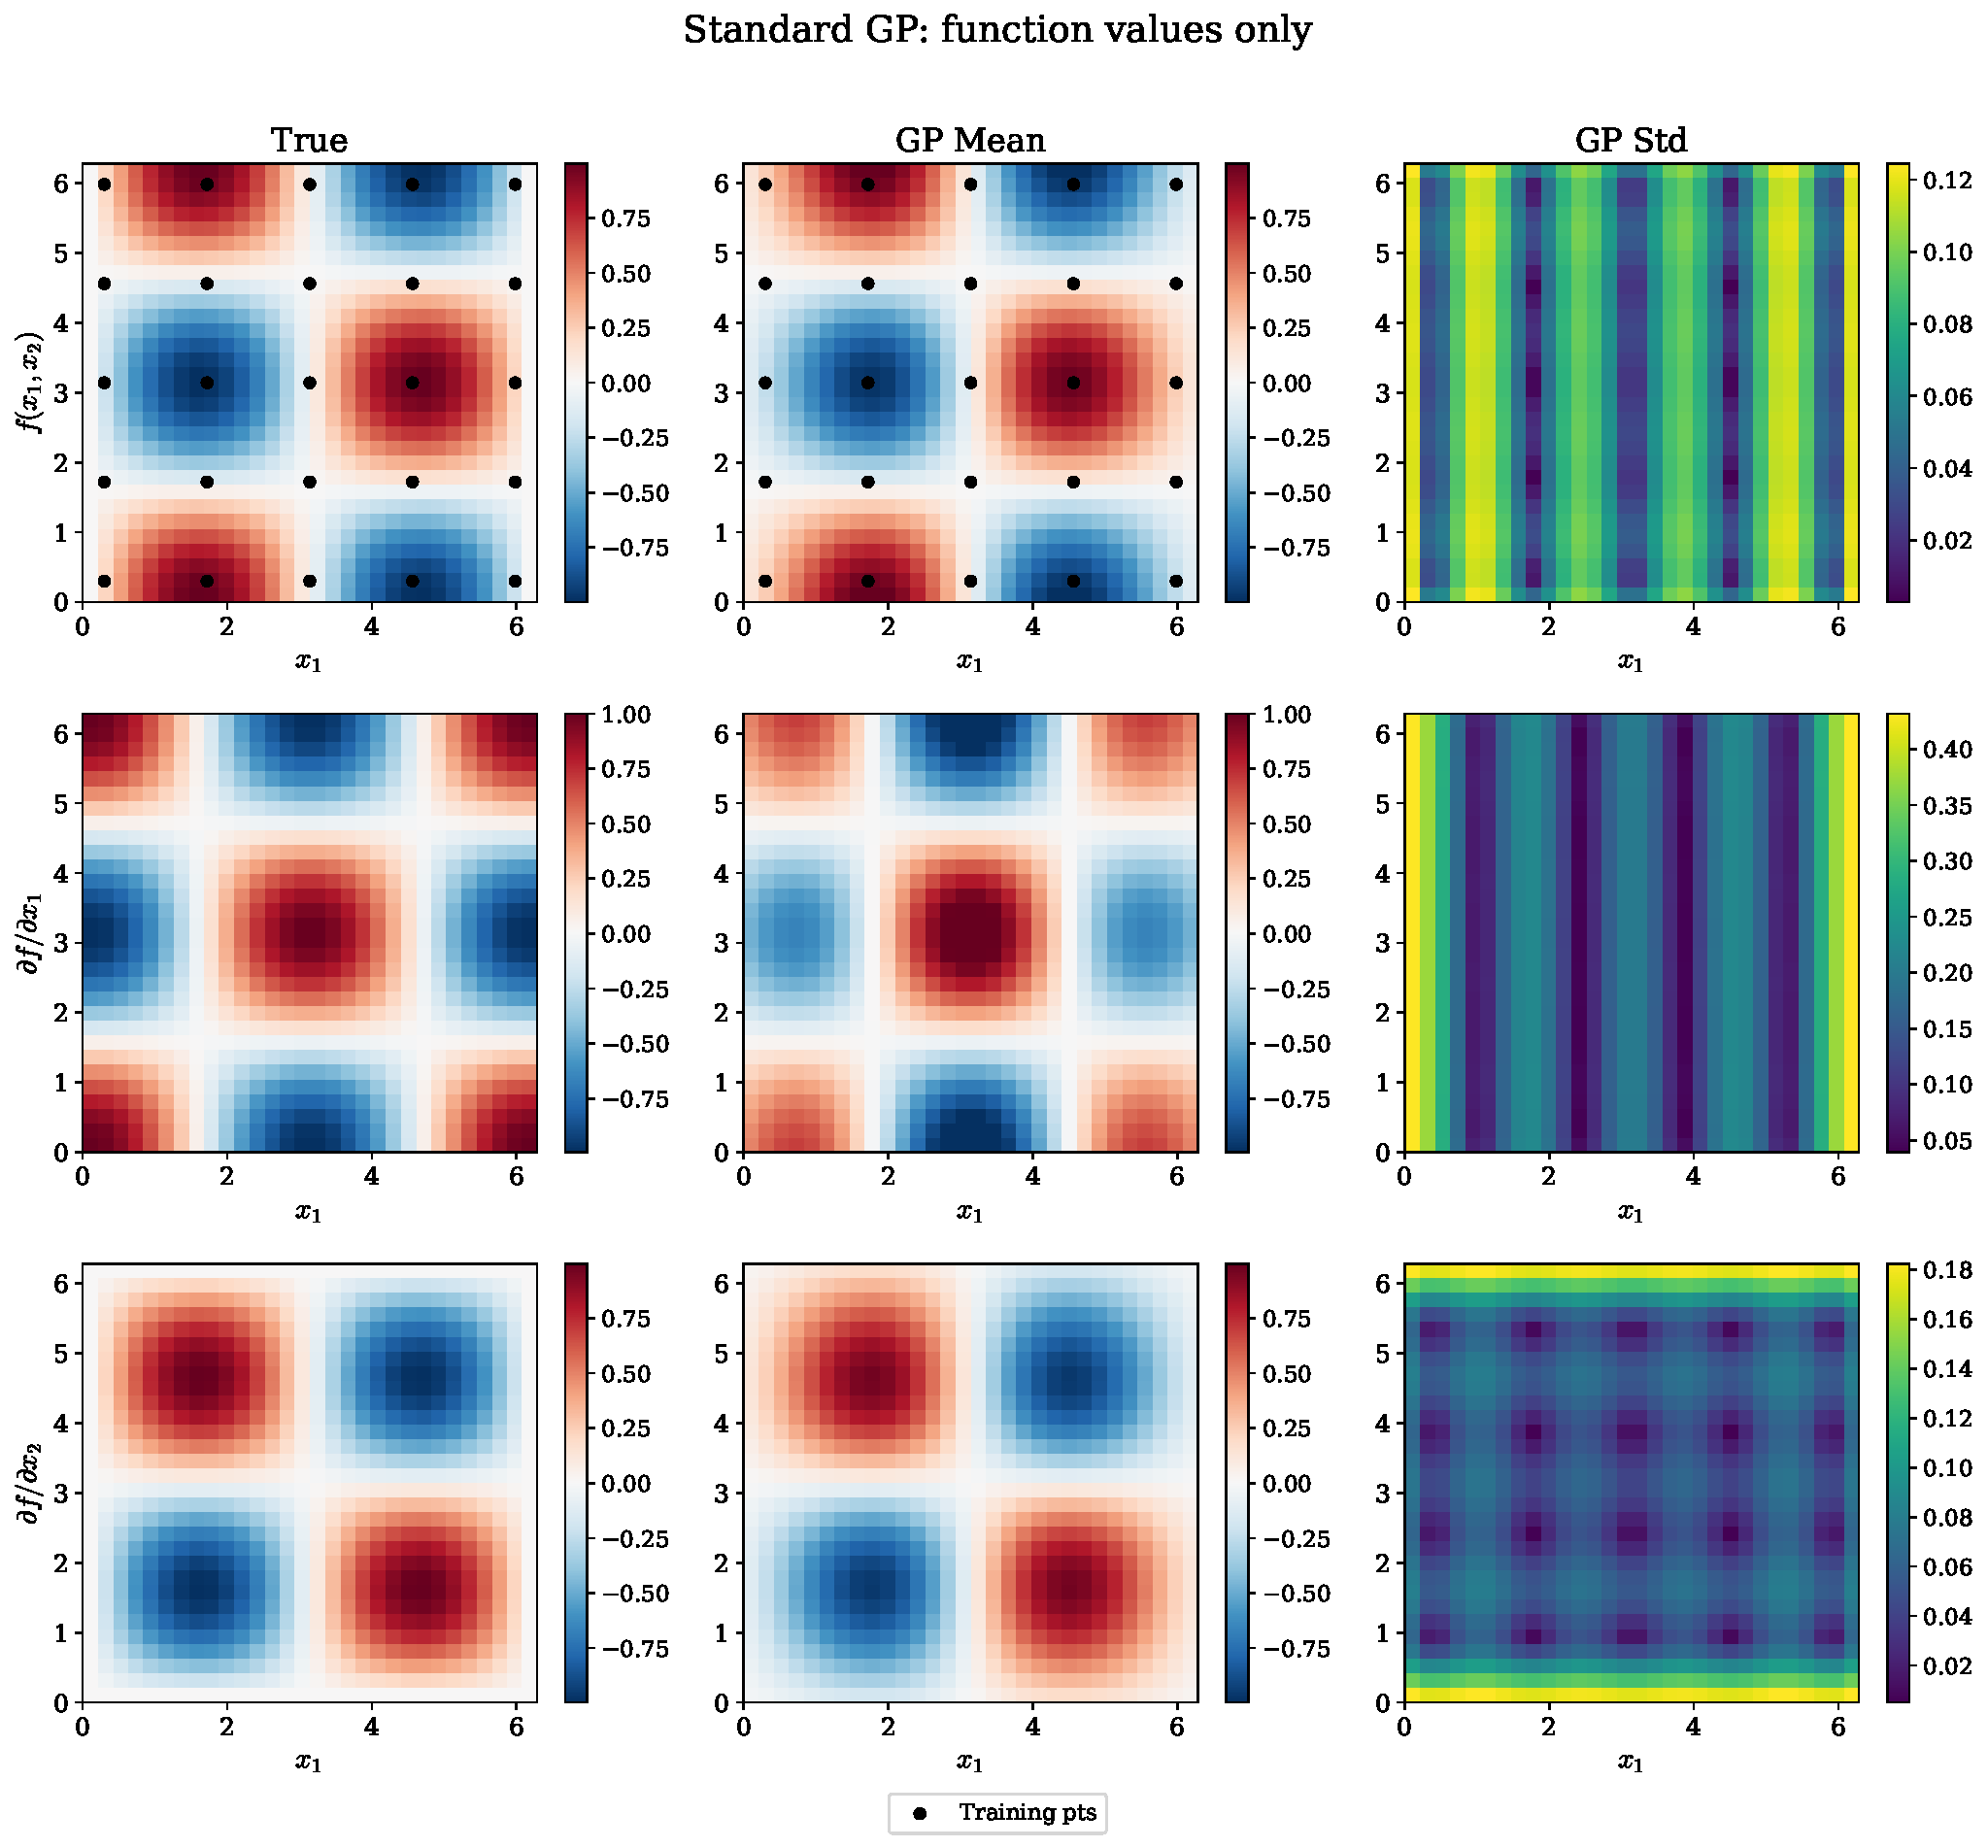
\includegraphics[width=\textwidth]{gp_example.pdf}
	\caption{Standard GP trained on $f(x_1, x_2) = \sin(x_1)\cos(x_2)$ with $n = 25$ function observations only (black dots). Rows show $f$, $\partial f / \partial x_1$, and $\partial f / \partial x_2$; columns show the true function, GP posterior mean, and posterior standard deviation. Derivative predictions are obtained via the cross-covariance structure described in Section~\ref{subsec:gp_deriv_pred}, without any derivative training data.}
	\label{fig:gp_example}
\end{figure}

\subsection{Gradient and Hessian Enhanced Gaussian Processes}
\label{subsec:grad_hess_gps}

\subsubsection{Gradient-Enhanced Gaussian Processes}
\label{subsec:derivative_gps}
When derivative information is available, it can be incorporated to improve model accuracy in high-dimensional or highly nonlinear problems~\cite{GEK, GHEK}. The most common approach involves including first-order gradient information, which has been shown to significantly improve the accuracy of GP models, particularly for functions with a high number of dimensions ($d \geq 8$)~\cite{Ulaganathan2016-xq}.

This is achieved by augmenting the observation vector to include the partial derivatives of the function at each training point, forming a Gradient-Enhanced GP (GEGP).

\begin{remark}[Derivative Notation]
	Throughout this work, the compact subscript notation for partial derivatives is adopted. For a kernel function $K(\mathbf{X}, \mathbf{X}')$, $\partial_{x_i} K$ is written in place of $\frac{\partial K}{\partial x_i}$, and $\partial^2_{x_i\,x_j'} K$ in place of $\frac{\partial^2 K}{\partial x_i \partial x_j'}$, with analogous notation for higher orders. Similarly, $\partial_{x_i} f(\mathbf{X})$ denotes the partial derivative vector $\frac{\partial f(\mathbf{X})}{\partial x_i}$. This notation extends naturally to directional derivatives, e.g., $\partial_{\mathbf{v}} f$ for $\frac{\partial f}{\partial \mathbf{v}}$, and to vector-valued subscripts denoting blocks of derivatives, e.g., $\partial_{\mathbf{X}'} K$ for the matrix of partial derivatives of $K$ with respect to all components of $\mathbf{X}'$.
\end{remark}

The observation vector $\mathbf{y}$ is expanded into an augmented vector, $\mathbf{y}^{G}$. In the general case, the predictions at the test locations $\mathbf{X}_*$ are also augmented to include derivatives, forming a vector $\mathbf{y}^{G}_*$, which enables simultaneous prediction of both function values and their partial derivatives:
\begin{equation}
	\label{eqn:gek_aug_vectors}
	\mathbf{y}^{G} = \begin{bmatrix} f(\mathbf{X}) \\ \partial_{x_1} f(\mathbf{X}) \\ \vdots \\ \partial_{x_d} f(\mathbf{X}) \end{bmatrix}, \quad
	\mathbf{y}^{G}_* = \begin{bmatrix} f(\mathbf{X}_*) \\ \partial_{x_1} f(\mathbf{X}_*) \\ \vdots \\ \partial_{x_d} f(\mathbf{X}_*) \end{bmatrix}.
\end{equation}
The joint distribution between the augmented training observations and the augmented test predictions is a multivariate Gaussian:
\begin{equation}
	\label{eqn:full_gek_joint_dist}
	\begin{pmatrix}
		\mathbf{y}^{G} \\
		\mathbf{y}^{G}_*
	\end{pmatrix}
	\sim \mathcal{N}\left(
	\mathbf{0},
	\begin{pmatrix}
		\boldsymbol{\Sigma}^{G}_{11} & \boldsymbol{\Sigma}^{G}_{12} \\
		\boldsymbol{\Sigma}^{G}_{21} & \boldsymbol{\Sigma}^{G}_{22}
	\end{pmatrix}
	\right).
\end{equation}
\begin{remark}[Kernel Argument Convention]
	Throughout this work, the kernel arguments are suppressed for brevity: it is understood that the entries of $\boldsymbol{\Sigma}_{11}$ are evaluated between training points $(\mathbf{X}, \mathbf{X}')$, those of $\boldsymbol{\Sigma}_{12}$ between training and test points $(\mathbf{X}, \mathbf{X}_*)$, and those of $\boldsymbol{\Sigma}_{22}$ between test points $(\mathbf{X}_*, \mathbf{X}_*')$.
\end{remark}

The blocks of this covariance matrix are also augmented. The training covariance block, $\boldsymbol{\Sigma}^{G}_{11}$, is an $n(d+1) \times n(d+1)$ matrix:
\begin{equation}
	\label{eqn:full_gek_S11}
	\boldsymbol{\Sigma}^{G}_{11} =
	\begin{pmatrix}
		K & \partial_{\mathbf{X}'} K \\
		\partial_{\mathbf{X}} K & \partial^2_{\mathbf{X}\,\mathbf{X}'} K
	\end{pmatrix}.
\end{equation}
The training-test covariance block is:
\begin{equation}
	\label{eqn:full_gek_S12}
	\boldsymbol{\Sigma}^{G}_{12} =
	\begin{pmatrix}
		K & \partial_{\mathbf{X}_*'} K \\
		\partial_{\mathbf{X}} K & \partial^2_{\mathbf{X}\,\mathbf{X}_*'} K
	\end{pmatrix},
\end{equation}
with $\boldsymbol{\Sigma}^{G}_{21} = \left(\boldsymbol{\Sigma}^{G}_{12}\right)^T$.

To make this concrete, consider a function of two variables ($d = 2$), for which the augmented training and test vectors take the explicit form:
\begin{equation}
	\label{eqn:gek_aug_vectors_2d}
	\mathbf{y}^{G} = \begin{bmatrix} f(\mathbf{X}) \\ \partial_{x_1} f(\mathbf{X}) \\ \partial_{x_2} f(\mathbf{X}) \end{bmatrix}, \quad
	\mathbf{y}^{G}_* = \begin{bmatrix} f(\mathbf{X}_*) \\ \partial_{x_1} f(\mathbf{X}_*) \\ \partial_{x_2} f(\mathbf{X}_*) \end{bmatrix},
\end{equation}
with their structure illustrated in Figure~\ref{fig:gek_aug_vectors_2d}.
\begin{figure}[htbp]
	\centering
	\begin{subfigure}[t]{0.45\textwidth}
		\centering
		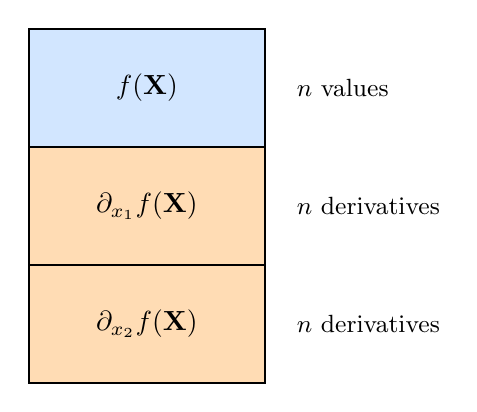
\begin{tikzpicture}
			\def\bw{3.0}
			\def\bh{1.5}
			
			\fill[ffblock] (0, 2*\bh) rectangle (\bw, 3*\bh);
			\fill[fdblock] (0, 1*\bh) rectangle (\bw, 2*\bh);
			\fill[fdblock] (0, 0*\bh) rectangle (\bw, 1*\bh);
			
			\draw[black, thick] (0, 0) rectangle (\bw, 3*\bh);
			\draw[black, thick] (0, \bh)   -- (\bw, \bh);
			\draw[black, thick] (0, 2*\bh) -- (\bw, 2*\bh);
			
			\node at (0.5*\bw, 2.5*\bh) {$f(\mathbf{X})$};
			\node at (0.5*\bw, 1.5*\bh) {$\partial_{x_1} f(\mathbf{X})$};
			\node at (0.5*\bw, 0.5*\bh) {$\partial_{x_2} f(\mathbf{X})$};

			\node[right=8pt, font=\small] at (\bw, 2.5*\bh) {$n$ values};
			\node[right=8pt, font=\small] at (\bw, 1.5*\bh) {$n$ derivatives};
			\node[right=8pt, font=\small] at (\bw, 0.5*\bh) {$n$ derivatives};
		\end{tikzpicture}
		\caption{Training vector $\mathbf{y}^{G}$}
		\label{fig:gek_training_vec_2d}
	\end{subfigure}
	\hfill
	\begin{subfigure}[t]{0.45\textwidth}
		\centering
		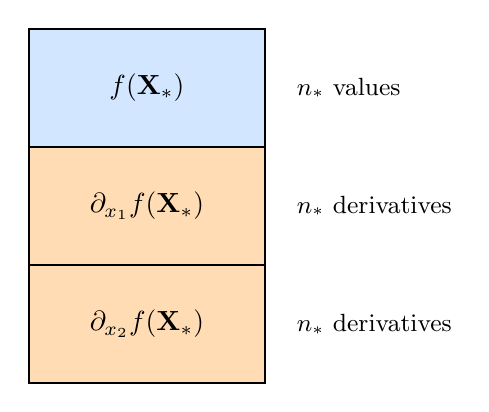
\begin{tikzpicture}
			\def\bw{3.0}
			\def\bh{1.5}

			\fill[ffblock] (0, 2*\bh) rectangle (\bw, 3*\bh);
			\fill[fdblock] (0, 1*\bh) rectangle (\bw, 2*\bh);
			\fill[fdblock] (0, 0*\bh) rectangle (\bw, 1*\bh);

			\draw[black, thick] (0, 0) rectangle (\bw, 3*\bh);
			\draw[black, thick] (0, \bh)   -- (\bw, \bh);
			\draw[black, thick] (0, 2*\bh) -- (\bw, 2*\bh);

			\node at (0.5*\bw, 2.5*\bh) {$f(\mathbf{X}_*)$};
			\node at (0.5*\bw, 1.5*\bh) {$\partial_{x_1} f(\mathbf{X}_*)$};
			\node at (0.5*\bw, 0.5*\bh) {$\partial_{x_2} f(\mathbf{X}_*)$};
			
			\node[right=8pt, font=\small] at (\bw, 2.5*\bh) {$n_*$ values};
			\node[right=8pt, font=\small] at (\bw, 1.5*\bh) {$n_*$ derivatives};
			\node[right=8pt, font=\small] at (\bw, 0.5*\bh) {$n_*$ derivatives};
			
		\end{tikzpicture}
		\caption{Test vector $\mathbf{y}^{G}_*$}
		\label{fig:gek_test_vec_2d}
	\end{subfigure}
	
	\caption{Structure of the augmented training and test vectors for a gradient-enhanced GP with $d=2$. Blue blocks contain function values at the $n$ training (or $n_*$ test) points, while orange blocks contain the corresponding partial derivatives with respect to each input dimension.}
	\label{fig:gek_aug_vectors_2d}
\end{figure}
The augmented training vector contains the function values and both partial derivatives at each training point, and the training covariance block $\boldsymbol{\Sigma}^{G}_{11}$ expands into a $3n \times 3n$ matrix with the following structure (see Figure~\ref{fig:gek_cov_structure}):
\begin{equation}
	\label{eqn:gek_S11_2d}
	\boldsymbol{\Sigma}^{G}_{11} =
	\begin{pmatrix}
		K &
		\partial_{x_1'} K &
		\partial_{x_2'} K \\[8pt]
		\partial_{x_1} K &
		\partial^2_{x_1\,x_1'} K &
		\partial^2_{x_1\,x_2'} K \\[8pt]
		\partial_{x_2} K &
		\partial^2_{x_2\,x_1'} K &
		\partial^2_{x_2\,x_2'} K
	\end{pmatrix}.
\end{equation}
\begin{figure}[htbp]
	\centering
	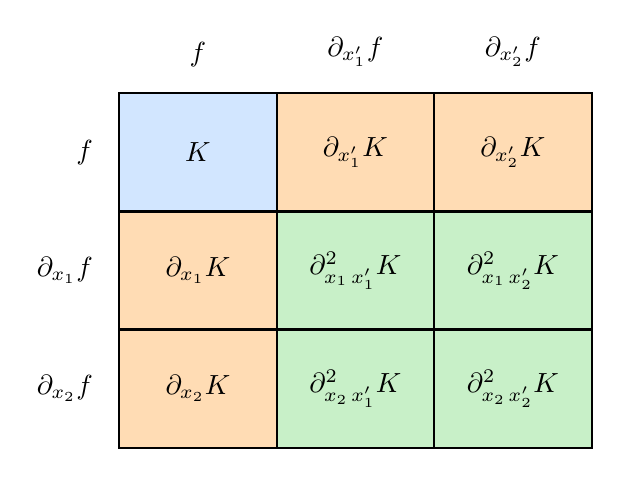
\begin{tikzpicture}
		\def\bw{2.0}  % block width
		\def\bh{1.5}  % block height
		
		% --- filled blocks ---
		% function-function (top-left)
		\fill[ffblock] (0,2*\bh) rectangle (\bw, 3*\bh);
		
		% function-derivative (top row, columns 2 and 3)
		\fill[fdblock] (\bw, 2*\bh)   rectangle (2*\bw, 3*\bh);
		\fill[fdblock] (2*\bw, 2*\bh) rectangle (3*\bw, 3*\bh);
		
		% derivative-function (left column, rows 2 and 3)
		\fill[fdblock] (0, \bh)   rectangle (\bw, 2*\bh);
		\fill[fdblock] (0, 0)     rectangle (\bw, \bh);
		
		% derivative-derivative (bottom-right 2x2)
		\fill[ddblock] (\bw, 0)     rectangle (2*\bw, \bh);
		\fill[ddblock] (\bw, \bh)   rectangle (2*\bw, 2*\bh);
		\fill[ddblock] (2*\bw, 0)   rectangle (3*\bw, \bh);
		\fill[ddblock] (2*\bw, \bh) rectangle (3*\bw, 2*\bh);
		
		% --- grid lines ---
		\draw[black, thick] (0,0) rectangle (3*\bw, 3*\bh);
		\draw[black, thick] (\bw, 0)   -- (\bw, 3*\bh);
		\draw[black, thick] (2*\bw, 0) -- (2*\bw, 3*\bh);
		\draw[black, thick] (0, \bh)   -- (3*\bw, \bh);
		\draw[black, thick] (0, 2*\bh) -- (3*\bw, 2*\bh);
		
		% --- labels ---
		\node at (0.5*\bw, 2.5*\bh) {$K$};
		
		\node at (1.5*\bw, 2.5*\bh) {$\partial_{x_1'} K$};
		\node at (2.5*\bw, 2.5*\bh) {$\partial_{x_2'} K$};

		\node at (0.5*\bw, 1.5*\bh) {$\partial_{x_1} K$};
		\node at (0.5*\bw, 0.5*\bh) {$\partial_{x_2} K$};

		\node at (1.5*\bw, 1.5*\bh) {$\partial^2_{x_1\,x_1'} K$};
		\node at (2.5*\bw, 1.5*\bh) {$\partial^2_{x_1\,x_2'} K$};
		\node at (1.5*\bw, 0.5*\bh) {$\partial^2_{x_2\,x_1'} K$};
		\node at (2.5*\bw, 0.5*\bh) {$\partial^2_{x_2\,x_2'} K$};
		
		% --- row/column headers ---
		\node[left=6pt] at (0, 2.5*\bh) {$f$};
		\node[left=6pt] at (0, 1.5*\bh) {$\partial_{x_1} f$};
		\node[left=6pt] at (0, 0.5*\bh) {$\partial_{x_2} f$};
		
		\node[above=6pt] at (0.5*\bw,  3*\bh) {$f$};
		\node[above=6pt] at (1.5*\bw,  3*\bh) {$\partial_{x_1'} f$};
		\node[above=6pt] at (2.5*\bw,  3*\bh) {$\partial_{x_2'} f$};
		
	\end{tikzpicture}
	
	% --- legend ---
	\vspace{8pt}
	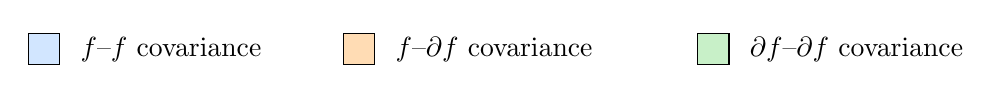
\begin{tikzpicture}
		\fill[ffblock] (0,0) rectangle (0.4, 0.4);
		\draw[black] (0,0) rectangle (0.4, 0.4);
		\node[right=4pt] at (0.4, 0.2) {$f$--$f$ covariance};
		
		\fill[fdblock] (4,0) rectangle (4.4, 0.4);
		\draw[black] (4,0) rectangle (4.4, 0.4);
		\node[right=4pt] at (4.4, 0.2) {$f$--$\partial f$ covariance};
		
		\fill[ddblock] (8.5,0) rectangle (8.9, 0.4);
		\draw[black] (8.5,0) rectangle (8.9, 0.4);
		\node[right=4pt] at (8.9, 0.2) {$\partial f$--$\partial f$ covariance};
	\end{tikzpicture}
	
	\caption{Block structure of the augmented training covariance matrix $\boldsymbol{\Sigma}^{G}_{11}$ for a two-dimensional input space ($d=2$). Blue, orange, and green shading denote the function--function, function--derivative, and derivative--derivative covariance blocks, respectively.}
	\label{fig:gek_cov_structure}
\end{figure}
This block structure extends naturally to arbitrary $d$, with one additional row and column of derivative covariance blocks per input dimension.

The posterior predictive distribution for the augmented test vector $\mathbf{y}^{G}_*$ is then given by:
\begin{equation}
	\label{eqn:full_gek_posterior}
	\begin{split}
		\boldsymbol{\mu}_{*} &= \boldsymbol{\Sigma}^{G}_{21} \left(\boldsymbol{\Sigma}^{G}_{11}\right)^{-1} \mathbf{y}^{G} \\
		\boldsymbol{\Sigma}_{*} &=  \boldsymbol{\Sigma}^{G}_{22} - \boldsymbol{\Sigma}^{G}_{21} \left(\boldsymbol{\Sigma}^{G}_{11}\right)^{-1} \boldsymbol{\Sigma}^{G}_{12}
	\end{split}
\end{equation}
The posterior mean $\boldsymbol{\mu}_{*}$ now provides predictions for both function values and derivatives, while $\boldsymbol{\Sigma}_{*}$ provides their uncertainty. The structure of both quantities is illustrated in Figure~\ref{fig:gek_posterior}.
\begin{figure}[htbp]
	\centering
\begin{subfigure}[t]{0.35\textwidth}
	\centering
	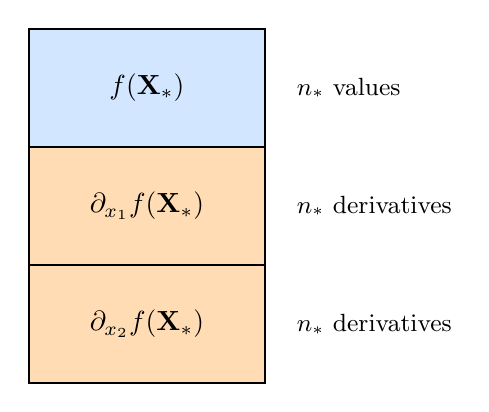
\begin{tikzpicture}
		\def\bw{3.0}  % wider to fit labels
		\def\bh{1.5}  % taller to fit fractions
		
		\fill[ffblock] (0, 2*\bh) rectangle (\bw, 3*\bh);
		\fill[fdblock] (0, 1*\bh) rectangle (\bw, 2*\bh);
		\fill[fdblock] (0, 0*\bh) rectangle (\bw, 1*\bh);
		
		\draw[black, thick] (0, 0) rectangle (\bw, 3*\bh);
		\draw[black, thick] (0, \bh)   -- (\bw, \bh);
		\draw[black, thick] (0, 2*\bh) -- (\bw, 2*\bh);
		
		\node at (0.5*\bw, 2.5*\bh) {$f(\mathbf{X}_*)$};
		\node at (0.5*\bw, 1.5*\bh) {$\partial_{x_1} f(\mathbf{X}_*)$};
		\node at (0.5*\bw, 0.5*\bh) {$\partial_{x_2} f(\mathbf{X}_*)$};
		
		% right-hand annotations
		\node[right=8pt, font=\small] at (\bw, 2.5*\bh) {$n_*$ values};
		\node[right=8pt, font=\small] at (\bw, 1.5*\bh) {$n_*$ derivatives};
		\node[right=8pt, font=\small] at (\bw, 0.5*\bh) {$n_*$ derivatives};
		
		
	\end{tikzpicture}
	\caption{Posterior mean $\boldsymbol{\mu}_*$}
	\label{fig:gek_posterior_mean}
\end{subfigure}
	\hfill
	\begin{subfigure}[t]{0.55\textwidth}
		\centering
		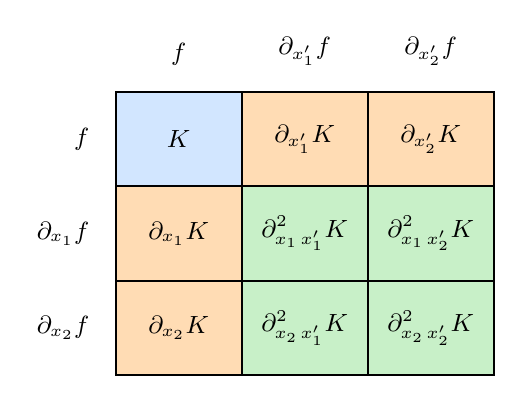
\begin{tikzpicture}
			\def\bw{1.6}
			\def\bh{1.2}
			
			% ff block
			\fill[ffblock] (0, 2*\bh) rectangle (\bw, 3*\bh);
			% fd blocks
			\fill[fdblock] (\bw, 2*\bh)   rectangle (2*\bw, 3*\bh);
			\fill[fdblock] (2*\bw, 2*\bh) rectangle (3*\bw, 3*\bh);
			\fill[fdblock] (0, \bh)        rectangle (\bw, 2*\bh);
			\fill[fdblock] (0, 0)          rectangle (\bw, \bh);
			% dd blocks
			\fill[ddblock] (\bw, 0)     rectangle (2*\bw, \bh);
			\fill[ddblock] (\bw, \bh)   rectangle (2*\bw, 2*\bh);
			\fill[ddblock] (2*\bw, 0)   rectangle (3*\bw, \bh);
			\fill[ddblock] (2*\bw, \bh) rectangle (3*\bw, 2*\bh);
			
			\draw[black, thick] (0,0) rectangle (3*\bw, 3*\bh);
			\draw[black, thick] (\bw, 0)   -- (\bw, 3*\bh);
			\draw[black, thick] (2*\bw, 0) -- (2*\bw, 3*\bh);
			\draw[black, thick] (0, \bh)   -- (3*\bw, \bh);
			\draw[black, thick] (0, 2*\bh) -- (3*\bw, 2*\bh);
			
			% cell labels
			\node[font=\small] at (0.5*\bw, 2.5*\bh) {$K$};
			\node[font=\small] at (1.5*\bw, 2.5*\bh) {$\partial_{x_1'} K$};
			\node[font=\small] at (2.5*\bw, 2.5*\bh) {$\partial_{x_2'} K$};
			\node[font=\small] at (0.5*\bw, 1.5*\bh) {$\partial_{x_1} K$};
			\node[font=\small] at (0.5*\bw, 0.5*\bh) {$\partial_{x_2} K$};
			\node[font=\small] at (1.5*\bw, 1.5*\bh) {$\partial^2_{x_1\,x_1'} K$};
			\node[font=\small] at (2.5*\bw, 1.5*\bh) {$\partial^2_{x_1\,x_2'} K$};
			\node[font=\small] at (1.5*\bw, 0.5*\bh) {$\partial^2_{x_2\,x_1'} K$};
			\node[font=\small] at (2.5*\bw, 0.5*\bh) {$\partial^2_{x_2\,x_2'} K$};
			
			% row/column headers
			\node[left=6pt, font=\small] at (0, 2.5*\bh) {$f$};
			\node[left=6pt, font=\small] at (0, 1.5*\bh) {$\partial_{x_1} f$};
			\node[left=6pt, font=\small] at (0, 0.5*\bh) {$\partial_{x_2} f$};
			
			\node[above=6pt, font=\small] at (0.5*\bw,  3*\bh) {$f$};
			\node[above=6pt, font=\small] at (1.5*\bw,  3*\bh) {$\partial_{x_1'} f$};
			\node[above=6pt, font=\small] at (2.5*\bw,  3*\bh) {$\partial_{x_2'} f$};


		\end{tikzpicture}
		\caption{Posterior covariance $\boldsymbol{\Sigma}_*$}
		\label{fig:gek_posterior_cov}
	\end{subfigure}
	
	\caption{Structure of the posterior predictive distribution for a gradient-enhanced GP with $d=2$. The posterior mean $\boldsymbol{\mu}_*$ (left) contains both function value and derivative predictions, while the posterior covariance $\boldsymbol{\Sigma}_*$ (right) captures the uncertainty in and between all predicted quantities, sharing the same block structure as $\boldsymbol{\Sigma}^{G}_{11}$ but evaluated at the test points $\mathbf{X}_*$.}
	\label{fig:gek_posterior}
\end{figure}
Similar to the standard GP, and assuming a noise-free model, the kernel hyperparameters $\boldsymbol{\psi}$ are determined by maximizing the log marginal likelihood (MLL) of the augmented observations:
\begin{equation}
	\label{eqn:gek_mll}
	\log p(\mathbf{y}^{G}|\mathbf{X}, \boldsymbol{\psi}) = -\frac{1}{2} \left(\mathbf{y}^{G}\right)^\top \left(\boldsymbol{\Sigma}^{G}_{11}\right)^{-1} \mathbf{y}^{G} - \frac{1}{2}\log|\boldsymbol{\Sigma}^{G}_{11}| - \frac{n(d+1)}{2}\log 2\pi.
\end{equation}
Evaluating this function during optimization is computationally demanding. The primary bottleneck is computing the inverse of $\boldsymbol{\Sigma}^{G}_{11}$ and the log-determinant $\log|\boldsymbol{\Sigma}^{G}_{11}|$, typically via Cholesky decomposition. The cost of this decomposition is approximately $O(M^3)$, where $M$ is the matrix dimension. For the gradient-enhanced case, $M = n(d+1)$, resulting in a cost of $O\left((n(d+1))^3\right)$. This cubic scaling with respect to both $n$ and $d$ makes hyperparameter optimization prohibitively expensive for problems with many data points or high dimensionality~\cite{FORRESTER200950, HeYouwei2023Aegk}.

\paragraph{Numerical example.}
To illustrate the GEGP, consider the test function $f(x_1, x_2) = \sin(x_1)\cos(x_2)$ on $[0, 2\pi]^2$. A $5 \times 5$ grid of training points ($n = 25$) is used, with function values and both partial derivatives observed at every point. The GP is trained with a squared exponential kernel and hyperparameters optimized via maximum likelihood. Figure~\ref{fig:gegp_example} shows the true function and partial derivatives alongside the GEGP predictions and predictive uncertainty. Incorporating gradient information at all training points yields highly accurate predictions of both the function and its derivatives, with near-zero predictive uncertainty near the training locations.

\begin{figure}[H]
	\centering
	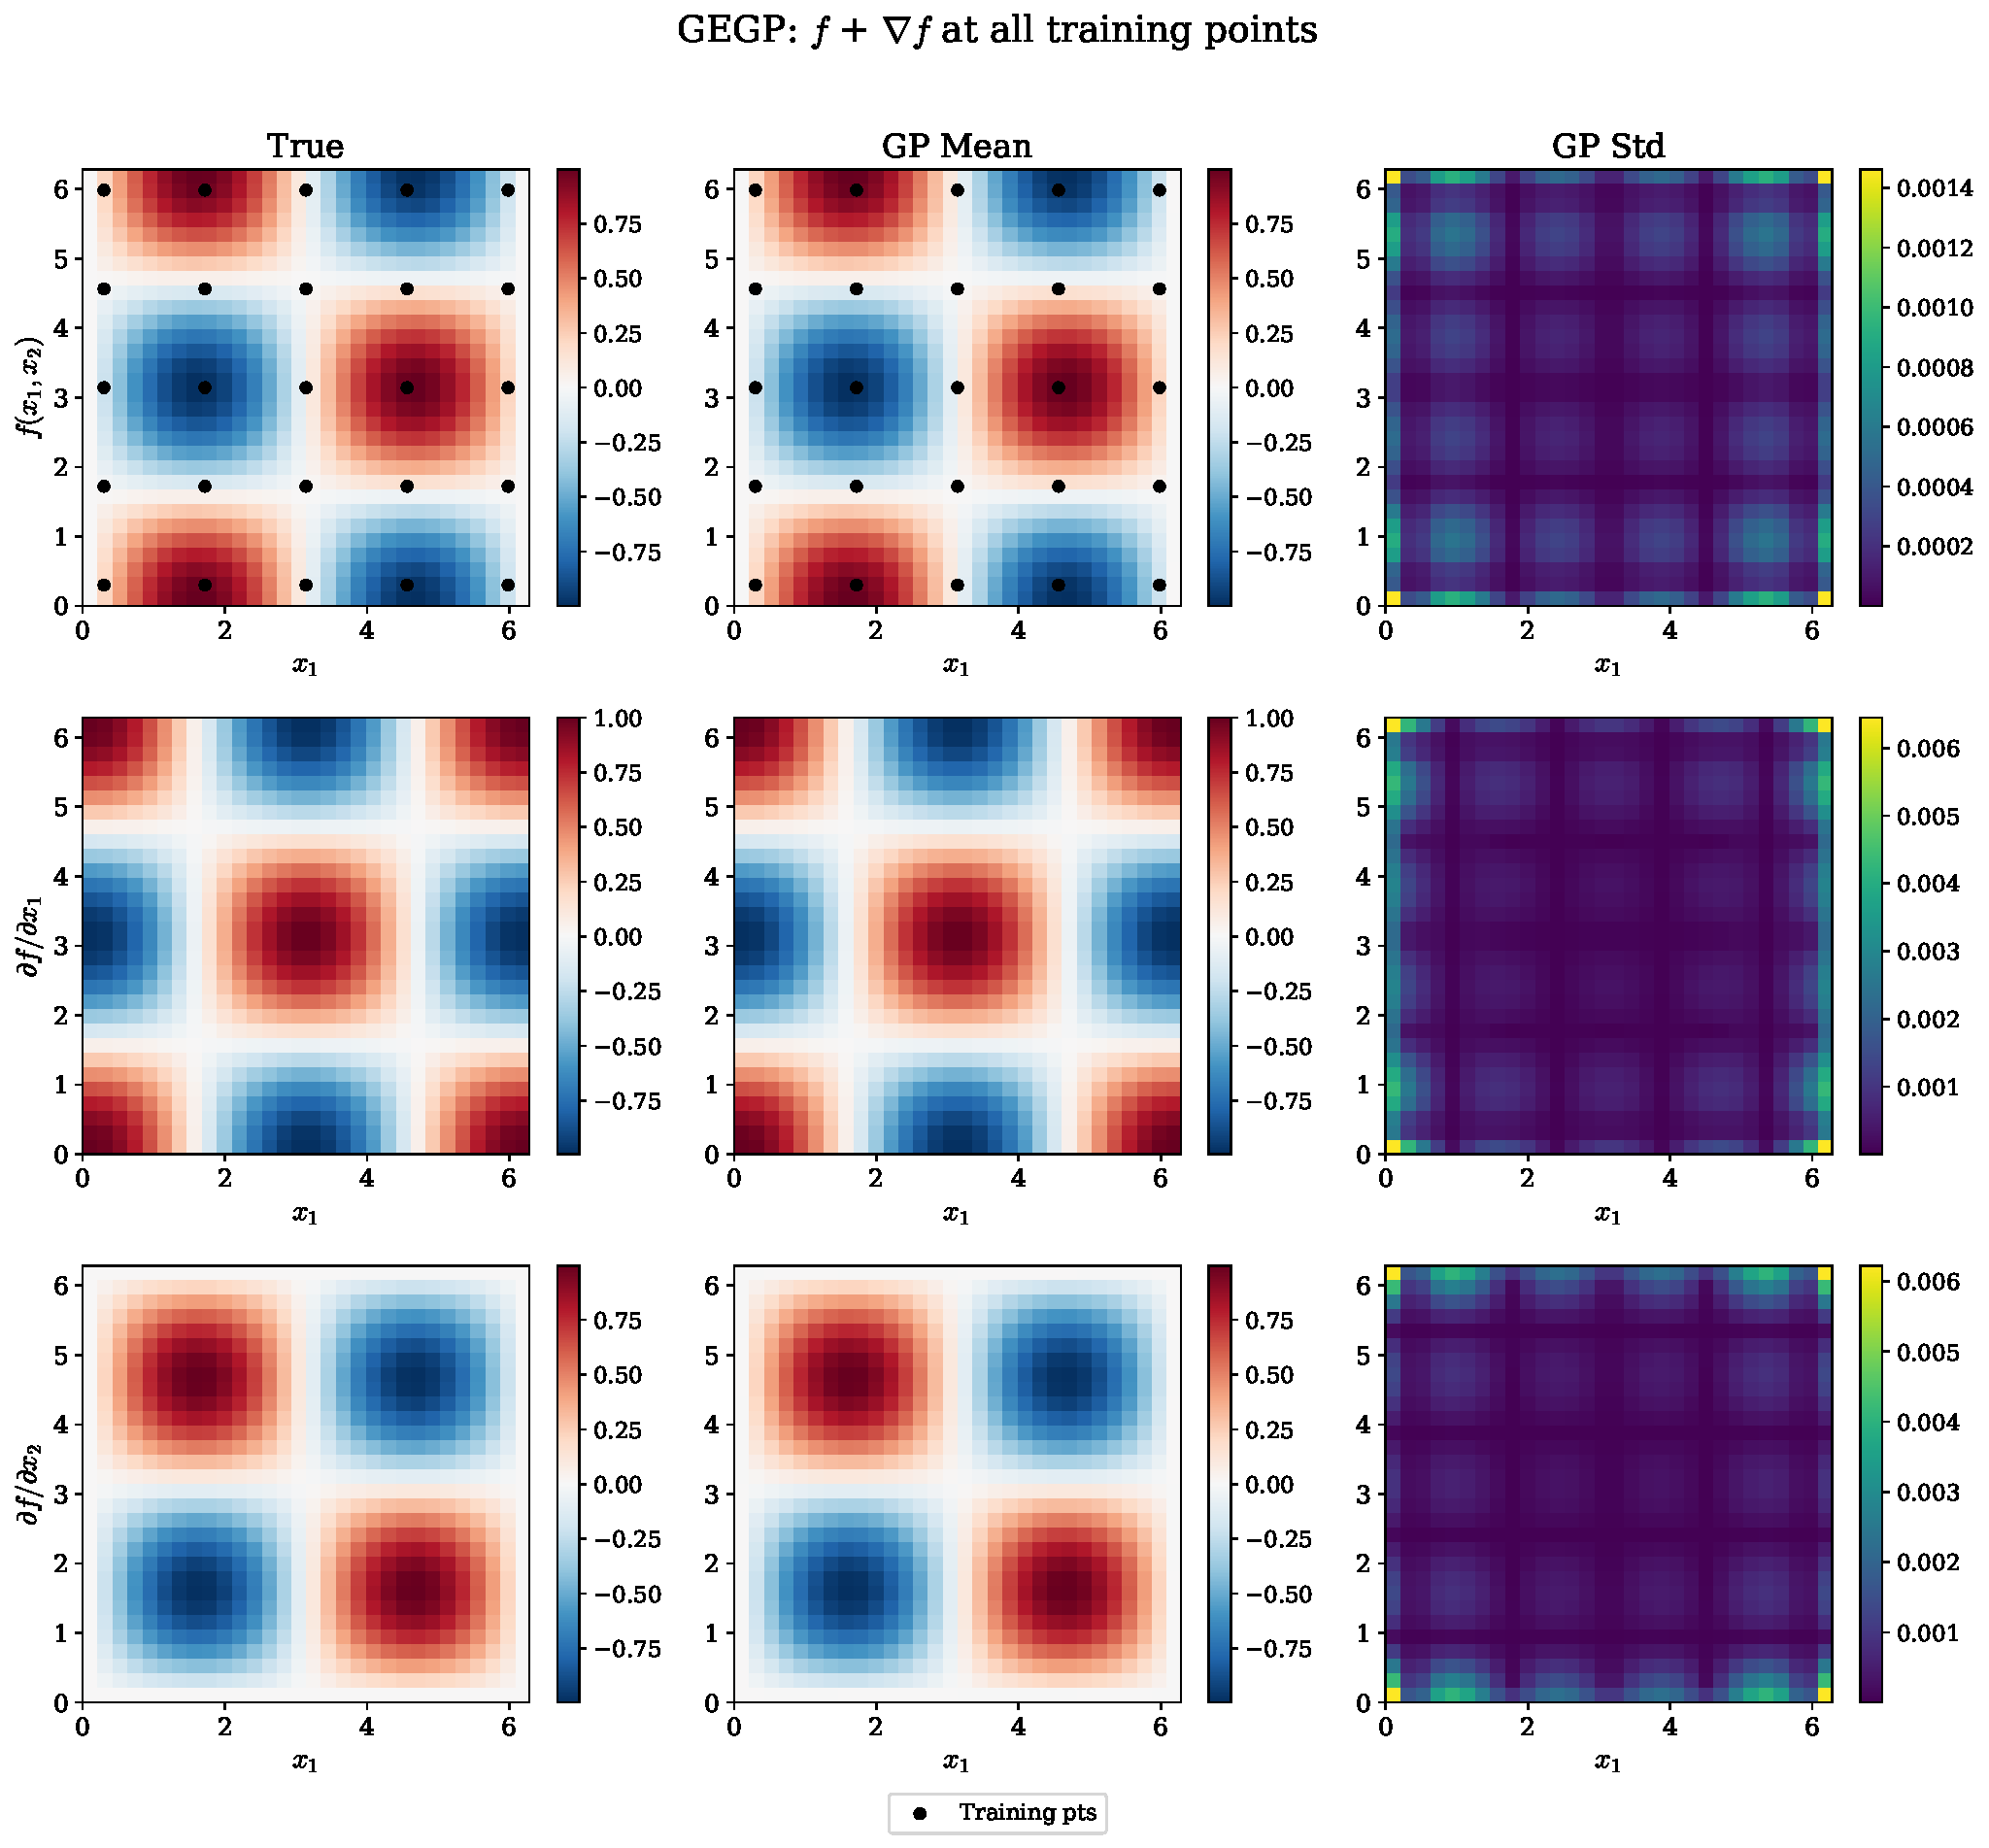
\includegraphics[width=\textwidth]{gegp_example.pdf}
	\caption{GEGP example on $f(x_1, x_2) = \sin(x_1)\cos(x_2)$ with $n = 25$ training points (black dots) and full gradient observations at every point. Rows show $f$, $\partial f / \partial x_1$, and $\partial f / \partial x_2$; columns show the true function, GP posterior mean, and posterior standard deviation.}
	\label{fig:gegp_example}
\end{figure}

\subsubsection{Hessian-Enhanced Gaussian Processes}
The framework can be further extended to include second-order derivative information (Hessians), forming a Hessian-Enhanced GP (HEGP), which is particularly useful for capturing behavior in highly nonlinear problems~\cite{GHEK}. This is achieved by further augmenting the observation vectors to include all function values, gradients, and unique Hessian components.
The augmented training vector, now denoted $\mathbf{y}^{H}$, concatenates the function values, gradients, and the $n \times d(d+1)/2$ unique components of the Hessian matrix from each of the $n$ training points. For a general model that also predicts these quantities, the test vector $\mathbf{y}^{H}_*$ is augmented similarly.

The joint distribution over these fully augmented vectors remains Gaussian, but the covariance matrix blocks are expanded further to include up to the fourth-order derivatives of the kernel function. The augmented training-training covariance block, $\boldsymbol{\Sigma}^{H}_{11}$, is a $3 \times 3$ block matrix with the following structure:
\begin{equation}
	\label{eqn:hegp_cov_matrix}
	\boldsymbol{\Sigma}^{H}_{11} =
	\begin{pmatrix}
		K & \partial_{\mathbf{X}'} K & \partial^2_{(\mathbf{X}')^2} K \\
		\partial_{\mathbf{X}} K & \partial^2_{\mathbf{X}\,\mathbf{X}'} K & \partial^3_{\mathbf{X}\,(\mathbf{X}')^2} K \\
		\partial^2_{\mathbf{X}^2} K & \partial^3_{\mathbf{X}^2\,\mathbf{X}'} K & \partial^4_{\mathbf{X}^2\,(\mathbf{X}')^2} K
	\end{pmatrix},
\end{equation}
The posterior predictive equations retain their standard form but now operate on these much larger matrices.

To make this concrete, for $d = 2$, the augmented training and test vectors take the explicit form:
\begin{equation}
	\label{eqn:hegp_aug_vectors_2d}
	\mathbf{y}^{H} = \begin{bmatrix} f(\mathbf{X}) \\ \partial_{x_1} f(\mathbf{X}) \\ \partial_{x_2} f(\mathbf{X}) \\ \partial^2_{x_1^2} f(\mathbf{X}) \\ \partial^2_{x_1\,x_2} f(\mathbf{X}) \\ \partial^2_{x_2^2} f(\mathbf{X}) \end{bmatrix}, \quad
	\mathbf{y}^{H}_* = \begin{bmatrix} f(\mathbf{X}_*) \\ \partial_{x_1} f(\mathbf{X}_*) \\ \partial_{x_2} f(\mathbf{X}_*) \\ \partial^2_{x_1^2} f(\mathbf{X}_*) \\ \partial^2_{x_1\,x_2} f(\mathbf{X}_*) \\ \partial^2_{x_2^2} f(\mathbf{X}_*) \end{bmatrix},
\end{equation}
with their structure illustrated in Figure~\ref{fig:hegp_aug_vectors_2d}.
\begin{figure}[H]
	\centering
	\begin{subfigure}[t]{0.45\textwidth}
		\centering
		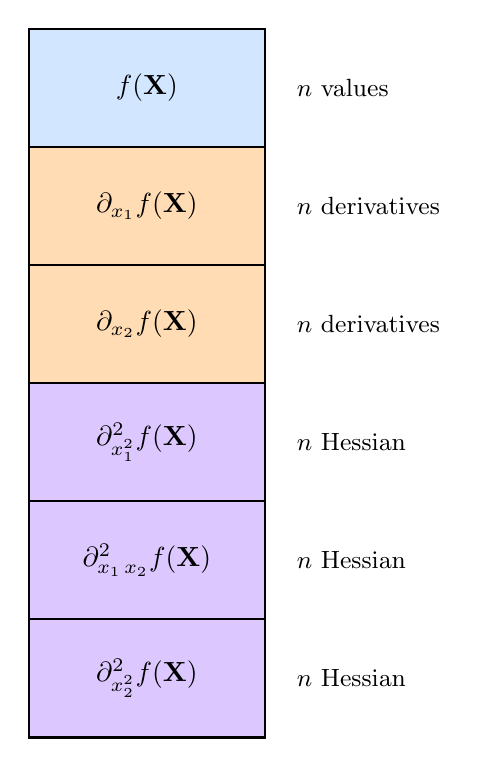
\begin{tikzpicture}
			\def\bw{3.0}
			\def\bh{1.5}
			
			\fill[ffblock] (0, 5*\bh) rectangle (\bw, 6*\bh);
			\fill[fdblock] (0, 4*\bh) rectangle (\bw, 5*\bh);
			\fill[fdblock] (0, 3*\bh) rectangle (\bw, 4*\bh);
			\fill[fhblock] (0, 2*\bh) rectangle (\bw, 3*\bh);
			\fill[fhblock] (0, 1*\bh) rectangle (\bw, 2*\bh);
			\fill[fhblock] (0, 0*\bh) rectangle (\bw, 1*\bh);
			
			\draw[black, thick] (0, 0) rectangle (\bw, 6*\bh);
			\foreach \i in {1,2,3,4,5} {
				\draw[black, thick] (0, \i*\bh) -- (\bw, \i*\bh);
			}
			
			\node at (0.5*\bw, 5.5*\bh) {$f(\mathbf{X})$};
			\node at (0.5*\bw, 4.5*\bh) {$\partial_{x_1} f(\mathbf{X})$};
			\node at (0.5*\bw, 3.5*\bh) {$\partial_{x_2} f(\mathbf{X})$};
			\node at (0.5*\bw, 2.5*\bh) {$\partial^2_{x_1^2} f(\mathbf{X})$};
			\node at (0.5*\bw, 1.5*\bh) {$\partial^2_{x_1\,x_2} f(\mathbf{X})$};
			\node at (0.5*\bw, 0.5*\bh) {$\partial^2_{x_2^2} f(\mathbf{X})$};
			
			\node[right=8pt, font=\small] at (\bw, 5.5*\bh) {$n$ values};
			\node[right=8pt, font=\small] at (\bw, 4.5*\bh) {$n$ derivatives};
			\node[right=8pt, font=\small] at (\bw, 3.5*\bh) {$n$ derivatives};
			\node[right=8pt, font=\small] at (\bw, 2.5*\bh) {$n$ Hessian};
			\node[right=8pt, font=\small] at (\bw, 1.5*\bh) {$n$ Hessian};
			\node[right=8pt, font=\small] at (\bw, 0.5*\bh) {$n$ Hessian};
			
		\end{tikzpicture}
		\caption{Training vector $\mathbf{y}^{H}$}
		\label{fig:hegp_training_vec_2d}
	\end{subfigure}
	\hfill
	\begin{subfigure}[t]{0.45\textwidth}
		\centering
		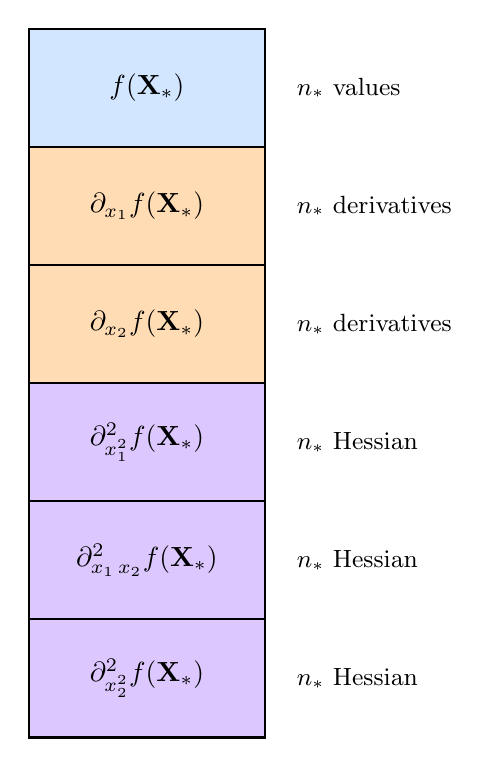
\begin{tikzpicture}
			\def\bw{3.0}
			\def\bh{1.5}
			
			\fill[ffblock] (0, 5*\bh) rectangle (\bw, 6*\bh);
			\fill[fdblock] (0, 4*\bh) rectangle (\bw, 5*\bh);
			\fill[fdblock] (0, 3*\bh) rectangle (\bw, 4*\bh);
			\fill[fhblock] (0, 2*\bh) rectangle (\bw, 3*\bh);
			\fill[fhblock] (0, 1*\bh) rectangle (\bw, 2*\bh);
			\fill[fhblock] (0, 0*\bh) rectangle (\bw, 1*\bh);
			
			\draw[black, thick] (0, 0) rectangle (\bw, 6*\bh);
			\foreach \i in {1,2,3,4,5} {
				\draw[black, thick] (0, \i*\bh) -- (\bw, \i*\bh);
			}
			
			\node at (0.5*\bw, 5.5*\bh) {$f(\mathbf{X}_*)$};
			\node at (0.5*\bw, 4.5*\bh) {$\partial_{x_1} f(\mathbf{X}_*)$};
			\node at (0.5*\bw, 3.5*\bh) {$\partial_{x_2} f(\mathbf{X}_*)$};
			\node at (0.5*\bw, 2.5*\bh) {$\partial^2_{x_1^2} f(\mathbf{X}_*)$};
			\node at (0.5*\bw, 1.5*\bh) {$\partial^2_{x_1\,x_2} f(\mathbf{X}_*)$};
			\node at (0.5*\bw, 0.5*\bh) {$\partial^2_{x_2^2} f(\mathbf{X}_*)$};
			
			\node[right=8pt, font=\small] at (\bw, 5.5*\bh) {$n_*$ values};
			\node[right=8pt, font=\small] at (\bw, 4.5*\bh) {$n_*$ derivatives};
			\node[right=8pt, font=\small] at (\bw, 3.5*\bh) {$n_*$ derivatives};
			\node[right=8pt, font=\small] at (\bw, 2.5*\bh) {$n_*$ Hessian};
			\node[right=8pt, font=\small] at (\bw, 1.5*\bh) {$n_*$ Hessian};
			\node[right=8pt, font=\small] at (\bw, 0.5*\bh) {$n_*$ Hessian};
			
		\end{tikzpicture}
		\caption{Test vector $\mathbf{y}^{H}_*$}
		\label{fig:hegp_test_vec_2d}
	\end{subfigure}
	
	\caption{Structure of the augmented training and test vectors for a Hessian-enhanced GP with $d=2$. Blue blocks contain function values, orange blocks contain first-order partial derivatives, and lavender blocks contain the three unique second-order partial derivatives (Hessian components) at each training or test point.}
	\label{fig:hegp_aug_vectors_2d}
\end{figure}
The augmented training vector contains the function value, two first-order partial derivatives, and three unique second-order partial derivatives at each training point, resulting in a $6n \times 6n$ training covariance block (see Figure~\ref{fig:hegp_cov_structure} for the corresponding block structure):
\begin{equation}
	\label{eqn:hegp_S11_2d}
	\boldsymbol{\Sigma}^{H}_{11} =
	\begin{pmatrix}
		K &
		\partial_{x_1'} K &
		\partial_{x_2'} K &
		\partial^2_{x_1'^2} K &
		\partial^2_{x_1'\,x_2'} K &
		\partial^2_{x_2'^2} K \\[8pt]
		%
		\partial_{x_1} K &
		\partial^2_{x_1\,x_1'} K &
		\partial^2_{x_1\,x_2'} K &
		\partial^3_{x_1\,x_1'^2} K &
		\partial^3_{x_1\,x_1'\,x_2'} K &
		\partial^3_{x_1\,x_2'^2} K \\[8pt]
		%
		\partial_{x_2} K &
		\partial^2_{x_2\,x_1'} K &
		\partial^2_{x_2\,x_2'} K &
		\partial^3_{x_2\,x_1'^2} K &
		\partial^3_{x_2\,x_1'\,x_2'} K &
		\partial^3_{x_2\,x_2'^2} K \\[8pt]
		%
		\partial^2_{x_1^2} K &
		\partial^3_{x_1^2\,x_1'} K &
		\partial^3_{x_1^2\,x_2'} K &
		\partial^4_{x_1^2\,x_1'^2} K &
		\partial^4_{x_1^2\,x_1'\,x_2'} K &
		\partial^4_{x_1^2\,x_2'^2} K \\[8pt]
		%
		\partial^2_{x_1\,x_2} K &
		\partial^3_{x_1\,x_2\,x_1'} K &
		\partial^3_{x_1\,x_2\,x_2'} K &
		\partial^4_{x_1\,x_2\,x_1'^2} K &
		\partial^4_{x_1\,x_2\,x_1'\,x_2'} K &
		\partial^4_{x_1\,x_2\,x_2'^2} K \\[8pt]
		%
		\partial^2_{x_2^2} K &
		\partial^3_{x_2^2\,x_1'} K &
		\partial^3_{x_2^2\,x_2'} K &
		\partial^4_{x_2^2\,x_1'^2} K &
		\partial^4_{x_2^2\,x_1'\,x_2'} K &
		\partial^4_{x_2^2\,x_2'^2} K
	\end{pmatrix},
\end{equation}

\begin{figure}[h!]
	\centering
	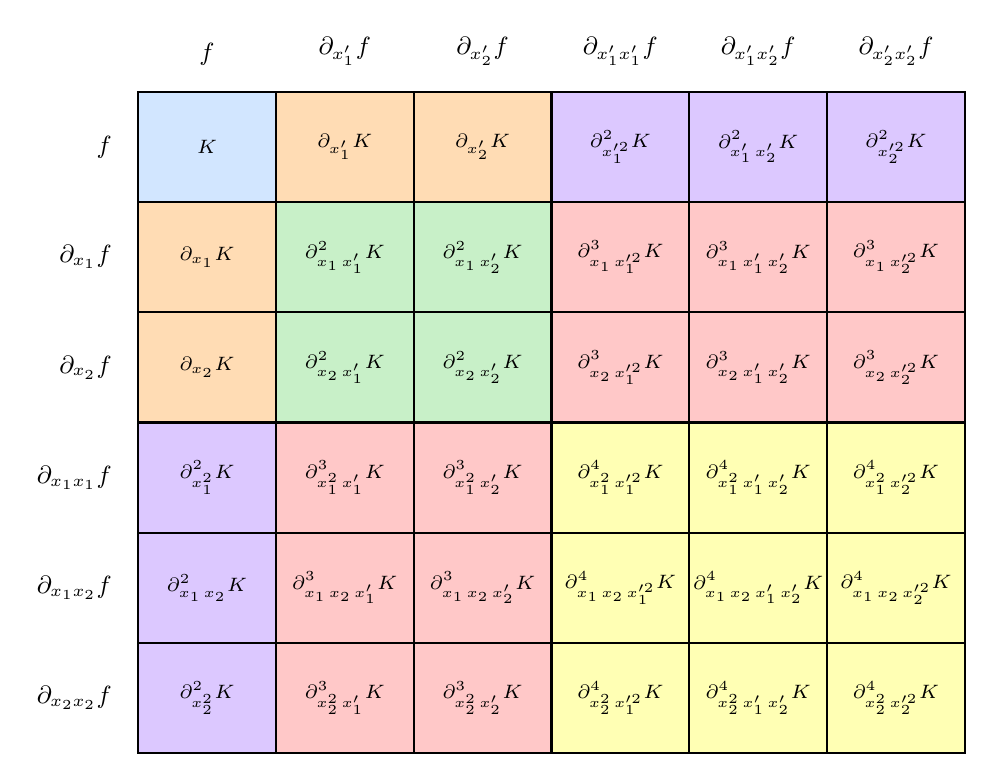
\begin{tikzpicture}
		\def\bw{1.75}  % block width
		\def\bh{1.4}  % block height
		
		% --- color map (row, col) -> color ---
		% Row/col order: f, dx1, dx2, dx1x1, dx1x2, dx2x2
		
		% Row 1: f
		\fill[ffblock] (0*\bw, 5*\bh) rectangle (1*\bw, 6*\bh);
		\fill[fdblock] (1*\bw, 5*\bh) rectangle (2*\bw, 6*\bh);
		\fill[fdblock] (2*\bw, 5*\bh) rectangle (3*\bw, 6*\bh);
		\fill[fhblock] (3*\bw, 5*\bh) rectangle (4*\bw, 6*\bh);
		\fill[fhblock] (4*\bw, 5*\bh) rectangle (5*\bw, 6*\bh);
		\fill[fhblock] (5*\bw, 5*\bh) rectangle (6*\bw, 6*\bh);
		
		% Row 2: dx1
		\fill[fdblock] (0*\bw, 4*\bh) rectangle (1*\bw, 5*\bh);
		\fill[ddblock] (1*\bw, 4*\bh) rectangle (2*\bw, 5*\bh);
		\fill[ddblock] (2*\bw, 4*\bh) rectangle (3*\bw, 5*\bh);
		\fill[ghblock] (3*\bw, 4*\bh) rectangle (4*\bw, 5*\bh);
		\fill[ghblock] (4*\bw, 4*\bh) rectangle (5*\bw, 5*\bh);
		\fill[ghblock] (5*\bw, 4*\bh) rectangle (6*\bw, 5*\bh);
		
		% Row 3: dx2
		\fill[fdblock] (0*\bw, 3*\bh) rectangle (1*\bw, 4*\bh);
		\fill[ddblock] (1*\bw, 3*\bh) rectangle (2*\bw, 4*\bh);
		\fill[ddblock] (2*\bw, 3*\bh) rectangle (3*\bw, 4*\bh);
		\fill[ghblock] (3*\bw, 3*\bh) rectangle (4*\bw, 4*\bh);
		\fill[ghblock] (4*\bw, 3*\bh) rectangle (5*\bw, 4*\bh);
		\fill[ghblock] (5*\bw, 3*\bh) rectangle (6*\bw, 4*\bh);
		
		% Row 4: dx1x1
		\fill[fhblock] (0*\bw, 2*\bh) rectangle (1*\bw, 3*\bh);
		\fill[ghblock] (1*\bw, 2*\bh) rectangle (2*\bw, 3*\bh);
		\fill[ghblock] (2*\bw, 2*\bh) rectangle (3*\bw, 3*\bh);
		\fill[hhblock] (3*\bw, 2*\bh) rectangle (4*\bw, 3*\bh);
		\fill[hhblock] (4*\bw, 2*\bh) rectangle (5*\bw, 3*\bh);
		\fill[hhblock] (5*\bw, 2*\bh) rectangle (6*\bw, 3*\bh);
		
		% Row 5: dx1x2
		\fill[fhblock] (0*\bw, 1*\bh) rectangle (1*\bw, 2*\bh);
		\fill[ghblock] (1*\bw, 1*\bh) rectangle (2*\bw, 2*\bh);
		\fill[ghblock] (2*\bw, 1*\bh) rectangle (3*\bw, 2*\bh);
		\fill[hhblock] (3*\bw, 1*\bh) rectangle (4*\bw, 2*\bh);
		\fill[hhblock] (4*\bw, 1*\bh) rectangle (5*\bw, 2*\bh);
		\fill[hhblock] (5*\bw, 1*\bh) rectangle (6*\bw, 2*\bh);
		
		% Row 6: dx2x2
		\fill[fhblock] (0*\bw, 0*\bh) rectangle (1*\bw, 1*\bh);
		\fill[ghblock] (1*\bw, 0*\bh) rectangle (2*\bw, 1*\bh);
		\fill[ghblock] (2*\bw, 0*\bh) rectangle (3*\bw, 1*\bh);
		\fill[hhblock] (3*\bw, 0*\bh) rectangle (4*\bw, 1*\bh);
		\fill[hhblock] (4*\bw, 0*\bh) rectangle (5*\bw, 1*\bh);
		\fill[hhblock] (5*\bw, 0*\bh) rectangle (6*\bw, 1*\bh);
		
		% --- grid lines ---
		\draw[black, thick] (0,0) rectangle (6*\bw, 6*\bh);
		\foreach \i in {1,2,3,4,5} {
			\draw[black, thick] (\i*\bw, 0) -- (\i*\bw, 6*\bh);
			\draw[black, thick] (0, \i*\bh) -- (6*\bw, \i*\bh);
		}
		
		% --- cell labels ---
		% Row f
		\node[font=\scriptsize] at (0.5*\bw, 5.5*\bh) {$K$};
		\node[font=\scriptsize] at (1.5*\bw, 5.5*\bh) {$\partial_{x_1'} K$};
		\node[font=\scriptsize] at (2.5*\bw, 5.5*\bh) {$\partial_{x_2'} K$};
		\node[font=\scriptsize] at (3.5*\bw, 5.5*\bh) {$\partial^2_{x_1'^2} K$};
		\node[font=\scriptsize] at (4.5*\bw, 5.5*\bh) {$\partial^2_{x_1'\,x_2'} K$};
		\node[font=\scriptsize] at (5.5*\bw, 5.5*\bh) {$\partial^2_{x_2'^2} K$};

		% Row dx1
		\node[font=\scriptsize] at (0.5*\bw, 4.5*\bh) {$\partial_{x_1} K$};
		\node[font=\scriptsize] at (1.5*\bw, 4.5*\bh) {$\partial^2_{x_1\,x_1'} K$};
		\node[font=\scriptsize] at (2.5*\bw, 4.5*\bh) {$\partial^2_{x_1\,x_2'} K$};
		\node[font=\scriptsize] at (3.5*\bw, 4.5*\bh) {$\partial^3_{x_1\,x_1'^2} K$};
		\node[font=\scriptsize] at (4.5*\bw, 4.5*\bh) {$\partial^3_{x_1\,x_1'\,x_2'} K$};
		\node[font=\scriptsize] at (5.5*\bw, 4.5*\bh) {$\partial^3_{x_1\,x_2'^2} K$};

		% Row dx2
		\node[font=\scriptsize] at (0.5*\bw, 3.5*\bh) {$\partial_{x_2} K$};
		\node[font=\scriptsize] at (1.5*\bw, 3.5*\bh) {$\partial^2_{x_2\,x_1'} K$};
		\node[font=\scriptsize] at (2.5*\bw, 3.5*\bh) {$\partial^2_{x_2\,x_2'} K$};
		\node[font=\scriptsize] at (3.5*\bw, 3.5*\bh) {$\partial^3_{x_2\,x_1'^2} K$};
		\node[font=\scriptsize] at (4.5*\bw, 3.5*\bh) {$\partial^3_{x_2\,x_1'\,x_2'} K$};
		\node[font=\scriptsize] at (5.5*\bw, 3.5*\bh) {$\partial^3_{x_2\,x_2'^2} K$};

		% Row dx1x1
		\node[font=\scriptsize] at (0.5*\bw, 2.5*\bh) {$\partial^2_{x_1^2} K$};
		\node[font=\scriptsize] at (1.5*\bw, 2.5*\bh) {$\partial^3_{x_1^2\,x_1'} K$};
		\node[font=\scriptsize] at (2.5*\bw, 2.5*\bh) {$\partial^3_{x_1^2\,x_2'} K$};
		\node[font=\scriptsize] at (3.5*\bw, 2.5*\bh) {$\partial^4_{x_1^2\,x_1'^2} K$};
		\node[font=\scriptsize] at (4.5*\bw, 2.5*\bh) {$\partial^4_{x_1^2\,x_1'\,x_2'} K$};
		\node[font=\scriptsize] at (5.5*\bw, 2.5*\bh) {$\partial^4_{x_1^2\,x_2'^2} K$};

		% Row dx1x2
		\node[font=\scriptsize] at (0.5*\bw, 1.5*\bh) {$\partial^2_{x_1\,x_2} K$};
		\node[font=\scriptsize] at (1.5*\bw, 1.5*\bh) {$\partial^3_{x_1\,x_2\,x_1'} K$};
		\node[font=\scriptsize] at (2.5*\bw, 1.5*\bh) {$\partial^3_{x_1\,x_2\,x_2'} K$};
		\node[font=\scriptsize] at (3.5*\bw, 1.5*\bh) {$\partial^4_{x_1\,x_2\,x_1'^2} K$};
		\node[font=\scriptsize] at (4.5*\bw, 1.5*\bh) {$\partial^4_{x_1\,x_2\,x_1'\,x_2'} K$};
		\node[font=\scriptsize] at (5.5*\bw, 1.5*\bh) {$\partial^4_{x_1\,x_2\,x_2'^2} K$};

		% Row dx2x2
		\node[font=\scriptsize] at (0.5*\bw, 0.5*\bh) {$\partial^2_{x_2^2} K$};
		\node[font=\scriptsize] at (1.5*\bw, 0.5*\bh) {$\partial^3_{x_2^2\,x_1'} K$};
		\node[font=\scriptsize] at (2.5*\bw, 0.5*\bh) {$\partial^3_{x_2^2\,x_2'} K$};
		\node[font=\scriptsize] at (3.5*\bw, 0.5*\bh) {$\partial^4_{x_2^2\,x_1'^2} K$};
		\node[font=\scriptsize] at (4.5*\bw, 0.5*\bh) {$\partial^4_{x_2^2\,x_1'\,x_2'} K$};
		\node[font=\scriptsize] at (5.5*\bw, 0.5*\bh) {$\partial^4_{x_2^2\,x_2'^2} K$};
		
		% --- row/column headers ---
		\node[left=6pt, font=\small] at (0, 5.5*\bh) {$f$};
		\node[left=6pt, font=\small] at (0, 4.5*\bh) {$\partial_{x_1} f$};
		\node[left=6pt, font=\small] at (0, 3.5*\bh) {$\partial_{x_2} f$};
		\node[left=6pt, font=\small] at (0, 2.5*\bh) {$\partial_{x_1 x_1} f$};
		\node[left=6pt, font=\small] at (0, 1.5*\bh) {$\partial_{x_1 x_2} f$};
		\node[left=6pt, font=\small] at (0, 0.5*\bh) {$\partial_{x_2 x_2} f$};
		
		\node[above=6pt, font=\small] at (0.5*\bw, 6*\bh) {$f$};
		\node[above=6pt, font=\small] at (1.5*\bw, 6*\bh) {$\partial_{x_1'} f$};
		\node[above=6pt, font=\small] at (2.5*\bw, 6*\bh) {$\partial_{x_2'} f$};
		\node[above=6pt, font=\small] at (3.5*\bw, 6*\bh) {$\partial_{x_1' x_1'} f$};
		\node[above=6pt, font=\small] at (4.5*\bw, 6*\bh) {$\partial_{x_1' x_2'} f$};
		\node[above=6pt, font=\small] at (5.5*\bw, 6*\bh) {$\partial_{x_2' x_2'} f$};
		
	\end{tikzpicture}
	
	% --- legend ---
	\vspace{8pt}
	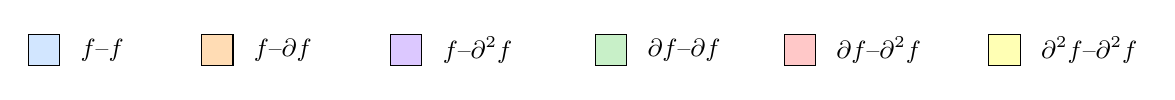
\begin{tikzpicture}
		\fill[ffblock] (0,0) rectangle (0.4,0.4);
		\draw[black] (0,0) rectangle (0.4,0.4);
		\node[right=4pt, font=\small] at (0.4,0.2) {$f$--$f$};
		
		\fill[fdblock] (2.2,0) rectangle (2.6,0.4);
		\draw[black] (2.2,0) rectangle (2.6,0.4);
		\node[right=4pt, font=\small] at (2.6,0.2) {$f$--$\partial f$};
		
		\fill[fhblock] (4.6,0) rectangle (5.0,0.4);
		\draw[black] (4.6,0) rectangle (5.0,0.4);
		\node[right=4pt, font=\small] at (5.0,0.2) {$f$--$\partial^2 f$};
		
		\fill[ddblock] (7.2,0) rectangle (7.6,0.4);
		\draw[black] (7.2,0) rectangle (7.6,0.4);
		\node[right=4pt, font=\small] at (7.6,0.2) {$\partial f$--$\partial f$};
		
		\fill[ghblock] (9.6,0) rectangle (10.0,0.4);
		\draw[black] (9.6,0) rectangle (10.0,0.4);
		\node[right=4pt, font=\small] at (10.0,0.2) {$\partial f$--$\partial^2 f$};
		
		\fill[hhblock] (12.2,0) rectangle (12.6,0.4);
		\draw[black] (12.2,0) rectangle (12.6,0.4);
		\node[right=4pt, font=\small] at (12.6,0.2) {$\partial^2 f$--$\partial^2 f$};
	\end{tikzpicture}
	
	\caption{Block structure of the augmented training covariance matrix $\boldsymbol{\Sigma}^{H}_{11}$ for a two-dimensional input space ($d=2$). The six shades correspond to the six distinct block types arising from combinations of function values, first-order partial derivatives, and second-order partial derivatives. Subscript notation $\partial_{ij'} K$ denotes $\partial^2 K / \partial x_i \partial x_j'$, with primes indicating differentiation with respect to the second argument.}
	\label{fig:hegp_cov_structure}
\end{figure}

The posterior predictive equations retain their standard forms, with computational cost scaling as $O\left((n(d(d+3)/2 + 1))^3\right)$.

\paragraph{Numerical example.}
Continuing with the same test function $f(x_1, x_2) = \sin(x_1)\cos(x_2)$ and the $5 \times 5$ training grid, the HEGP augments the training data with all three unique second-order partial derivatives ($\partial^2 f / \partial x_1^2$, $\partial^2 f / \partial x_1 \partial x_2$, $\partial^2 f / \partial x_2^2$) in addition to function values and gradients. Figure~\ref{fig:hegp_example} shows the resulting predictions. Compared to the GEGP (Figure~\ref{fig:gegp_example}), the inclusion of curvature information reduces prediction error by several orders of magnitude and produces near-machine-precision reconstruction of the function and its first derivatives.

\begin{figure}[p]
	\centering
	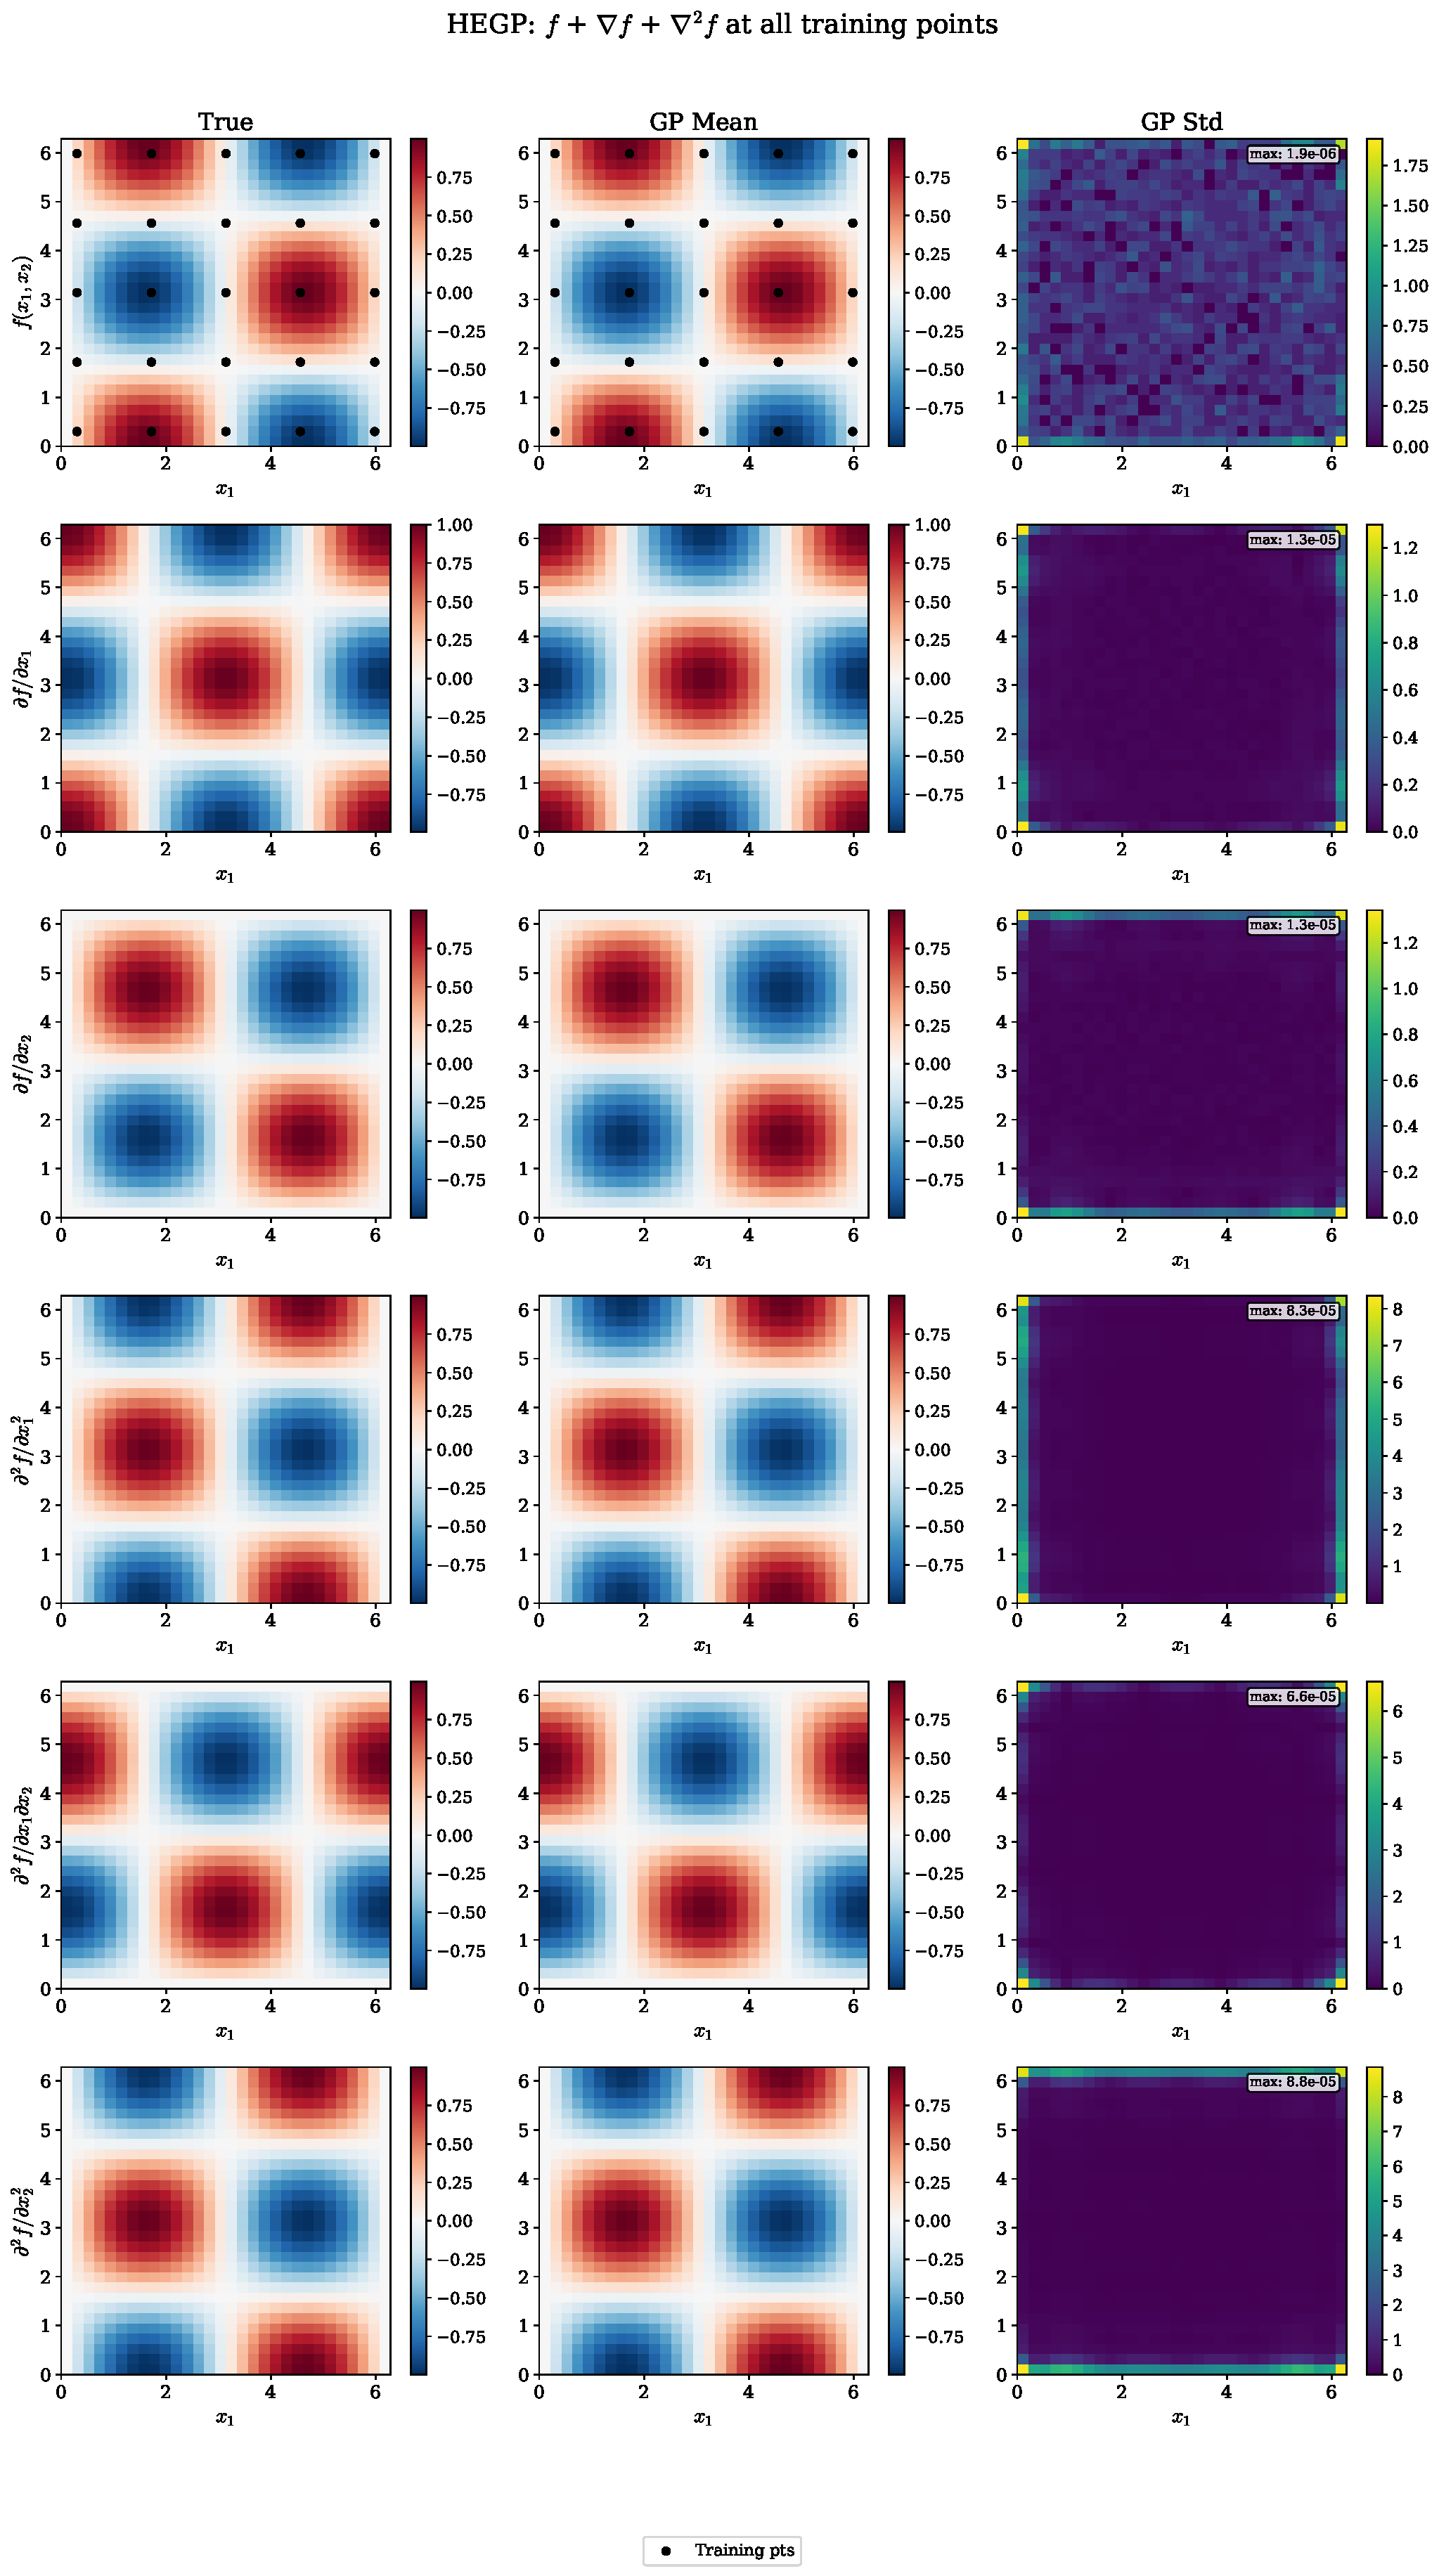
\includegraphics[width=\textwidth,height=0.9\textheight,keepaspectratio]{hegp_example.pdf}
	\caption{HEGP example on $f(x_1, x_2) = \sin(x_1)\cos(x_2)$ with $n = 25$ training points and full gradient and Hessian observations. Rows show $f$, $\partial f / \partial x_1$, $\partial f / \partial x_2$, $\partial^2 f / \partial x_1^2$, $\partial^2 f / \partial x_1 \partial x_2$, and $\partial^2 f / \partial x_2^2$; columns show the true function, GP posterior mean, and posterior standard deviation. The inclusion of second-order derivatives dramatically reduces predictive uncertainty compared to the GEGP in Figure~\ref{fig:gegp_example}.}
	\label{fig:hegp_example}
\end{figure}

\subsubsection{Selective Derivative Predictions at Test Locations}
\label{subsec:selective_deriv_pred}
In many applications, only the function values $f(\mathbf{X}_*)$ are required at the test points, not their derivatives. In this case, the augmented training-test covariance blocks $\boldsymbol{\Sigma}_{12}^{(\cdot)}$ simplify by retaining only the columns corresponding to the test function values, while still leveraging derivative information from the training points. Additionally, the test-test covariance block $\boldsymbol{\Sigma}_{22}^{(\cdot)}$ reduces to the standard form $K$, since no derivatives are predicted at the test locations.

For a GEGP, the full training-test block is
\begin{equation}
	\boldsymbol{\Sigma}_{12}^{G} =
	\begin{pmatrix}
		K & \partial_{\mathbf{X}_*'} K \\
		\partial_{\mathbf{X}} K & \partial^2_{\mathbf{X}\,\mathbf{X}_*'} K
	\end{pmatrix},
\end{equation}
When only $f(\mathbf{X}_*)$ is needed, the training-test and test-test covariance blocks reduce to
\begin{equation}
	\boldsymbol{\Sigma}_{12}^{G} \;\longrightarrow\;
	\begin{pmatrix}
		K \\
		\partial_{\mathbf{X}} K
	\end{pmatrix}, \quad \text{and} \quad
	\boldsymbol{\Sigma}_{22}^{G} \;\longrightarrow\; K.
\end{equation}
The block structure of both the full and reduced forms is illustrated in Figure~\ref{fig:gek_s12_reduction}.

\begin{figure}[htbp]
	\centering
	\begin{subfigure}[t]{0.45\textwidth}
		\centering
		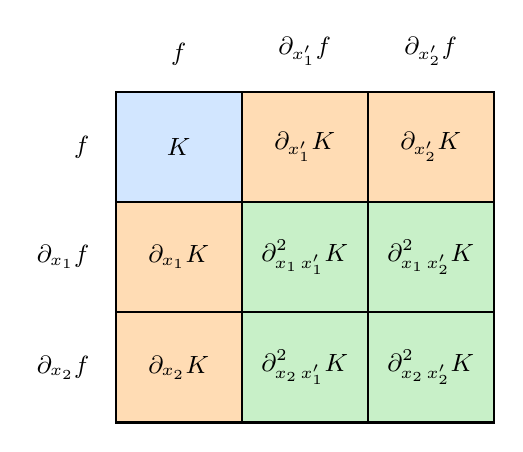
\begin{tikzpicture}
			\def\bw{1.6}
			\def\bh{1.4}
			
			% Full Sigma_12^G: 3x3, same structure as Sigma_11
			% Row 1: f
			\fill[ffblock] (0, 2*\bh) rectangle (\bw, 3*\bh);
			\fill[fdblock] (\bw, 2*\bh) rectangle (2*\bw, 3*\bh);
			\fill[fdblock] (2*\bw, 2*\bh) rectangle (3*\bw, 3*\bh);
			% Row 2: dx1
			\fill[fdblock] (0, \bh) rectangle (\bw, 2*\bh);
			\fill[ddblock] (\bw, \bh) rectangle (2*\bw, 2*\bh);
			\fill[ddblock] (2*\bw, \bh) rectangle (3*\bw, 2*\bh);
			% Row 3: dx2
			\fill[fdblock] (0, 0) rectangle (\bw, \bh);
			\fill[ddblock] (\bw, 0) rectangle (2*\bw, \bh);
			\fill[ddblock] (2*\bw, 0) rectangle (3*\bw, \bh);
			
			\draw[black, thick] (0,0) rectangle (3*\bw, 3*\bh);
			\draw[black, thick] (\bw, 0) -- (\bw, 3*\bh);
			\draw[black, thick] (2*\bw, 0) -- (2*\bw, 3*\bh);
			\draw[black, thick] (0, \bh) -- (3*\bw, \bh);
			\draw[black, thick] (0, 2*\bh) -- (3*\bw, 2*\bh);
			
			\node[font=\small] at (0.5*\bw, 2.5*\bh) {$K$};
			\node[font=\small] at (1.5*\bw, 2.5*\bh) {$\partial_{x_1'} K$};
			\node[font=\small] at (2.5*\bw, 2.5*\bh) {$\partial_{x_2'} K$};
			\node[font=\small] at (0.5*\bw, 1.5*\bh) {$\partial_{x_1} K$};
			\node[font=\small] at (1.5*\bw, 1.5*\bh) {$\partial^2_{x_1\,x_1'} K$};
			\node[font=\small] at (2.5*\bw, 1.5*\bh) {$\partial^2_{x_1\,x_2'} K$};
			\node[font=\small] at (0.5*\bw, 0.5*\bh) {$\partial_{x_2} K$};
			\node[font=\small] at (1.5*\bw, 0.5*\bh) {$\partial^2_{x_2\,x_1'} K$};
			\node[font=\small] at (2.5*\bw, 0.5*\bh) {$\partial^2_{x_2\,x_2'} K$};

			\node[left=6pt, font=\small] at (0, 2.5*\bh) {$f$};
			\node[left=6pt, font=\small] at (0, 1.5*\bh) {$\partial_{x_1} f$};
			\node[left=6pt, font=\small] at (0, 0.5*\bh) {$\partial_{x_2} f$};

			\node[above=6pt, font=\small] at (0.5*\bw, 3*\bh) {$f$};
			\node[above=6pt, font=\small] at (1.5*\bw, 3*\bh) {$\partial_{x_1'} f$};
			\node[above=6pt, font=\small] at (2.5*\bw, 3*\bh) {$\partial_{x_2'} f$};

		\end{tikzpicture}
		\caption{Full $\boldsymbol{\Sigma}^{G}_{12}$}
	\end{subfigure}
	\hfill
	\begin{subfigure}[t]{0.45\textwidth}
		\centering
		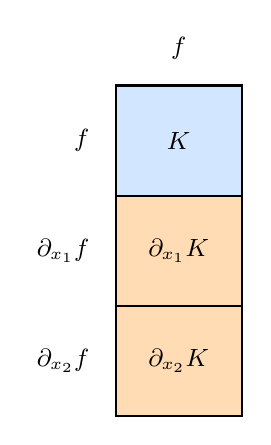
\begin{tikzpicture}
			\def\bw{1.6}
			\def\bh{1.4}

			% Reduced Sigma_12^G: 3x1, first column only
			\fill[ffblock] (0, 2*\bh) rectangle (\bw, 3*\bh);
			\fill[fdblock] (0, \bh) rectangle (\bw, 2*\bh);
			\fill[fdblock] (0, 0) rectangle (\bw, \bh);

			\draw[black, thick] (0,0) rectangle (\bw, 3*\bh);
			\draw[black, thick] (0, \bh) -- (\bw, \bh);
			\draw[black, thick] (0, 2*\bh) -- (\bw, 2*\bh);

			\node[font=\small] at (0.5*\bw, 2.5*\bh) {$K$};
			\node[font=\small] at (0.5*\bw, 1.5*\bh) {$\partial_{x_1} K$};
			\node[font=\small] at (0.5*\bw, 0.5*\bh) {$\partial_{x_2} K$};
			
			\node[left=6pt, font=\small] at (0, 2.5*\bh) {$f$};
			\node[left=6pt, font=\small] at (0, 1.5*\bh) {$\partial_{x_1} f$};
			\node[left=6pt, font=\small] at (0, 0.5*\bh) {$\partial_{x_2} f$};
			
			\node[above=6pt, font=\small] at (0.5*\bw, 3*\bh) {$f$};
			
		\end{tikzpicture}
		\caption{Reduced $\boldsymbol{\Sigma}^{G}_{12}$}
	\end{subfigure}
	\caption{Full (left) and reduced (right) training-test covariance block $\boldsymbol{\Sigma}^{G}_{12}$ for a GEGP with $d=2$, when only function values are predicted at test locations. The reduced form retains only the first column of blocks, reducing from a $3n \times 3n_*$ matrix to a $3n \times n_*$ matrix.}
	\label{fig:gek_s12_reduction}
\end{figure}

For a HEGP, the full block is
\begin{equation}
	\boldsymbol{\Sigma}_{12}^{H} =
	\begin{pmatrix}
		K & \partial_{\mathbf{X}_*'} K & \partial^2_{(\mathbf{X}_*')^2} K \\
		\partial_{\mathbf{X}} K & \partial^2_{\mathbf{X}\,\mathbf{X}_*'} K & \partial^3_{\mathbf{X}\,(\mathbf{X}_*')^2} K \\
		\partial^2_{\mathbf{X}^2} K & \partial^3_{\mathbf{X}^2\,\mathbf{X}_*'} K & \partial^4_{\mathbf{X}^2\,(\mathbf{X}_*')^2} K
	\end{pmatrix},
\end{equation}
When only $f(\mathbf{X}_*)$ is needed, the training-test and test-test covariance blocks reduce to
\begin{equation}
	\boldsymbol{\Sigma}_{12}^{H} \;\longrightarrow\;
	\begin{pmatrix}
		K \\
		\partial_{\mathbf{X}} K \\
		\partial^2_{\mathbf{X}^2} K
	\end{pmatrix}, \quad \text{and} \quad
	\boldsymbol{\Sigma}_{22}^{H} \;\longrightarrow\; K.
\end{equation}
The corresponding block structures are illustrated in Figure~\ref{fig:hegp_s12_reduction}.
\begin{figure}[h!]
	\centering
	\begin{subfigure}[t]{0.65\textwidth}
		\centering
		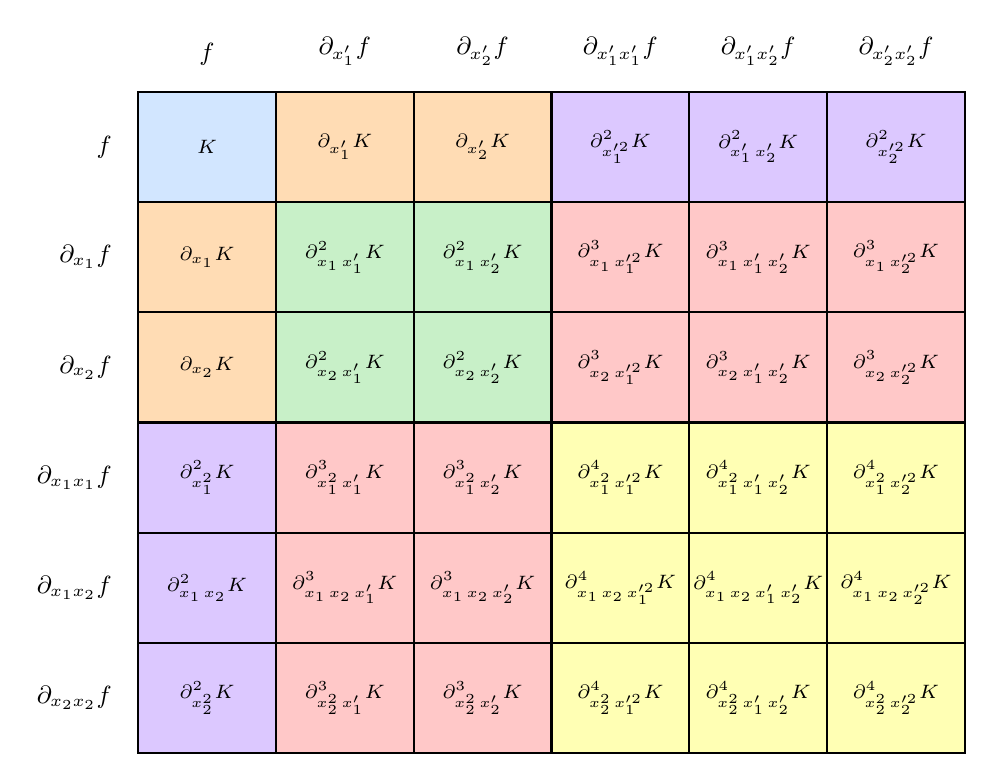
\begin{tikzpicture}
			\def\bw{1.75}
			\def\bh{1.4}


			% Full Sigma_12^H: 6x6, same structure as Sigma_11^H
			% Row 1: f
			\fill[ffblock] (0*\bw, 5*\bh) rectangle (1*\bw, 6*\bh);
			\fill[fdblock] (1*\bw, 5*\bh) rectangle (2*\bw, 6*\bh);
			\fill[fdblock] (2*\bw, 5*\bh) rectangle (3*\bw, 6*\bh);
			\fill[fhblock] (3*\bw, 5*\bh) rectangle (4*\bw, 6*\bh);
			\fill[fhblock] (4*\bw, 5*\bh) rectangle (5*\bw, 6*\bh);
			\fill[fhblock] (5*\bw, 5*\bh) rectangle (6*\bw, 6*\bh);
			% Row 2: dx1
			\fill[fdblock] (0*\bw, 4*\bh) rectangle (1*\bw, 5*\bh);
			\fill[ddblock] (1*\bw, 4*\bh) rectangle (2*\bw, 5*\bh);
			\fill[ddblock] (2*\bw, 4*\bh) rectangle (3*\bw, 5*\bh);
			\fill[ghblock] (3*\bw, 4*\bh) rectangle (4*\bw, 5*\bh);
			\fill[ghblock] (4*\bw, 4*\bh) rectangle (5*\bw, 5*\bh);
			\fill[ghblock] (5*\bw, 4*\bh) rectangle (6*\bw, 5*\bh);
			% Row 3: dx2
			\fill[fdblock] (0*\bw, 3*\bh) rectangle (1*\bw, 4*\bh);
			\fill[ddblock] (1*\bw, 3*\bh) rectangle (2*\bw, 4*\bh);
			\fill[ddblock] (2*\bw, 3*\bh) rectangle (3*\bw, 4*\bh);
			\fill[ghblock] (3*\bw, 3*\bh) rectangle (4*\bw, 4*\bh);
			\fill[ghblock] (4*\bw, 3*\bh) rectangle (5*\bw, 4*\bh);
			\fill[ghblock] (5*\bw, 3*\bh) rectangle (6*\bw, 4*\bh);
			% Row 4: dx1x1
			\fill[fhblock] (0*\bw, 2*\bh) rectangle (1*\bw, 3*\bh);
			\fill[ghblock] (1*\bw, 2*\bh) rectangle (2*\bw, 3*\bh);
			\fill[ghblock] (2*\bw, 2*\bh) rectangle (3*\bw, 3*\bh);
			\fill[hhblock] (3*\bw, 2*\bh) rectangle (4*\bw, 3*\bh);
			\fill[hhblock] (4*\bw, 2*\bh) rectangle (5*\bw, 3*\bh);
			\fill[hhblock] (5*\bw, 2*\bh) rectangle (6*\bw, 3*\bh);
			% Row 5: dx1x2
			\fill[fhblock] (0*\bw, 1*\bh) rectangle (1*\bw, 2*\bh);
			\fill[ghblock] (1*\bw, 1*\bh) rectangle (2*\bw, 2*\bh);
			\fill[ghblock] (2*\bw, 1*\bh) rectangle (3*\bw, 2*\bh);
			\fill[hhblock] (3*\bw, 1*\bh) rectangle (4*\bw, 2*\bh);
			\fill[hhblock] (4*\bw, 1*\bh) rectangle (5*\bw, 2*\bh);
			\fill[hhblock] (5*\bw, 1*\bh) rectangle (6*\bw, 2*\bh);
			% Row 6: dx2x2
			\fill[fhblock] (0*\bw, 0*\bh) rectangle (1*\bw, 1*\bh);
			\fill[ghblock] (1*\bw, 0*\bh) rectangle (2*\bw, 1*\bh);
			\fill[ghblock] (2*\bw, 0*\bh) rectangle (3*\bw, 1*\bh);
			\fill[hhblock] (3*\bw, 0*\bh) rectangle (4*\bw, 1*\bh);
			\fill[hhblock] (4*\bw, 0*\bh) rectangle (5*\bw, 1*\bh);
			\fill[hhblock] (5*\bw, 0*\bh) rectangle (6*\bw, 1*\bh);
			
			\draw[black, thick] (0,0) rectangle (6*\bw, 6*\bh);
			\foreach \i in {1,2,3,4,5} {
				\draw[black, thick] (\i*\bw, 0) -- (\i*\bw, 6*\bh);
				\draw[black, thick] (0, \i*\bh) -- (6*\bw, \i*\bh);
			}

			% --- cell labels ---
			% Row f
			\node[font=\scriptsize] at (0.5*\bw, 5.5*\bh) {$K$};
			\node[font=\scriptsize] at (1.5*\bw, 5.5*\bh) {$\partial_{x_1'} K$};
			\node[font=\scriptsize] at (2.5*\bw, 5.5*\bh) {$\partial_{x_2'} K$};
			\node[font=\scriptsize] at (3.5*\bw, 5.5*\bh) {$\partial^2_{x_1'^2} K$};
			\node[font=\scriptsize] at (4.5*\bw, 5.5*\bh) {$\partial^2_{x_1'\,x_2'} K$};
			\node[font=\scriptsize] at (5.5*\bw, 5.5*\bh) {$\partial^2_{x_2'^2} K$};
			% Row dx1
			\node[font=\scriptsize] at (0.5*\bw, 4.5*\bh) {$\partial_{x_1} K$};
			\node[font=\scriptsize] at (1.5*\bw, 4.5*\bh) {$\partial^2_{x_1\,x_1'} K$};
			\node[font=\scriptsize] at (2.5*\bw, 4.5*\bh) {$\partial^2_{x_1\,x_2'} K$};
			\node[font=\scriptsize] at (3.5*\bw, 4.5*\bh) {$\partial^3_{x_1\,x_1'^2} K$};
			\node[font=\scriptsize] at (4.5*\bw, 4.5*\bh) {$\partial^3_{x_1\,x_1'\,x_2'} K$};
			\node[font=\scriptsize] at (5.5*\bw, 4.5*\bh) {$\partial^3_{x_1\,x_2'^2} K$};
			% Row dx2
			\node[font=\scriptsize] at (0.5*\bw, 3.5*\bh) {$\partial_{x_2} K$};
			\node[font=\scriptsize] at (1.5*\bw, 3.5*\bh) {$\partial^2_{x_2\,x_1'} K$};
			\node[font=\scriptsize] at (2.5*\bw, 3.5*\bh) {$\partial^2_{x_2\,x_2'} K$};
			\node[font=\scriptsize] at (3.5*\bw, 3.5*\bh) {$\partial^3_{x_2\,x_1'^2} K$};
			\node[font=\scriptsize] at (4.5*\bw, 3.5*\bh) {$\partial^3_{x_2\,x_1'\,x_2'} K$};
			\node[font=\scriptsize] at (5.5*\bw, 3.5*\bh) {$\partial^3_{x_2\,x_2'^2} K$};
			% Row dx1x1
			\node[font=\scriptsize] at (0.5*\bw, 2.5*\bh) {$\partial^2_{x_1^2} K$};
			\node[font=\scriptsize] at (1.5*\bw, 2.5*\bh) {$\partial^3_{x_1^2\,x_1'} K$};
			\node[font=\scriptsize] at (2.5*\bw, 2.5*\bh) {$\partial^3_{x_1^2\,x_2'} K$};
			\node[font=\scriptsize] at (3.5*\bw, 2.5*\bh) {$\partial^4_{x_1^2\,x_1'^2} K$};
			\node[font=\scriptsize] at (4.5*\bw, 2.5*\bh) {$\partial^4_{x_1^2\,x_1'\,x_2'} K$};
			\node[font=\scriptsize] at (5.5*\bw, 2.5*\bh) {$\partial^4_{x_1^2\,x_2'^2} K$};
			% Row dx1x2
			\node[font=\scriptsize] at (0.5*\bw, 1.5*\bh) {$\partial^2_{x_1\,x_2} K$};
			\node[font=\scriptsize] at (1.5*\bw, 1.5*\bh) {$\partial^3_{x_1\,x_2\,x_1'} K$};
			\node[font=\scriptsize] at (2.5*\bw, 1.5*\bh) {$\partial^3_{x_1\,x_2\,x_2'} K$};
			\node[font=\scriptsize] at (3.5*\bw, 1.5*\bh) {$\partial^4_{x_1\,x_2\,x_1'^2} K$};
			\node[font=\scriptsize] at (4.5*\bw, 1.5*\bh) {$\partial^4_{x_1\,x_2\,x_1'\,x_2'} K$};
			\node[font=\scriptsize] at (5.5*\bw, 1.5*\bh) {$\partial^4_{x_1\,x_2\,x_2'^2} K$};
			% Row dx2x2
			\node[font=\scriptsize] at (0.5*\bw, 0.5*\bh) {$\partial^2_{x_2^2} K$};
			\node[font=\scriptsize] at (1.5*\bw, 0.5*\bh) {$\partial^3_{x_2^2\,x_1'} K$};
			\node[font=\scriptsize] at (2.5*\bw, 0.5*\bh) {$\partial^3_{x_2^2\,x_2'} K$};
			\node[font=\scriptsize] at (3.5*\bw, 0.5*\bh) {$\partial^4_{x_2^2\,x_1'^2} K$};
			\node[font=\scriptsize] at (4.5*\bw, 0.5*\bh) {$\partial^4_{x_2^2\,x_1'\,x_2'} K$};
			\node[font=\scriptsize] at (5.5*\bw, 0.5*\bh) {$\partial^4_{x_2^2\,x_2'^2} K$};

			\node[left=6pt, font=\small] at (0, 5.5*\bh) {$f$};
			\node[left=6pt, font=\small] at (0, 4.5*\bh) {$\partial_{x_1} f$};
			\node[left=6pt, font=\small] at (0, 3.5*\bh) {$\partial_{x_2} f$};
			\node[left=6pt, font=\small] at (0, 2.5*\bh) {$\partial_{x_1x_1} f$};
			\node[left=6pt, font=\small] at (0, 1.5*\bh) {$\partial_{x_1x_2} f$};
			\node[left=6pt, font=\small] at (0, 0.5*\bh) {$\partial_{x_2x_2} f$};

			\node[above=6pt, font=\small] at (0.5*\bw, 6*\bh) {$f$};
			\node[above=6pt, font=\small] at (1.5*\bw, 6*\bh) {$\partial_{x_1'} f$};
			\node[above=6pt, font=\small] at (2.5*\bw, 6*\bh) {$\partial_{x_2'} f$};
			\node[above=6pt, font=\small] at (3.5*\bw, 6*\bh) {$\partial_{x_1'x_1'} f$};
			\node[above=6pt, font=\small] at (4.5*\bw, 6*\bh) {$\partial_{x_1'x_2'} f$};
			\node[above=6pt, font=\small] at (5.5*\bw, 6*\bh) {$\partial_{x_2'x_2'} f$};


		\end{tikzpicture}
		\caption{Full $\boldsymbol{\Sigma}^{H}_{12}$}
	\end{subfigure}
	\hfill
	\begin{subfigure}[t]{0.30\textwidth}
		\centering
		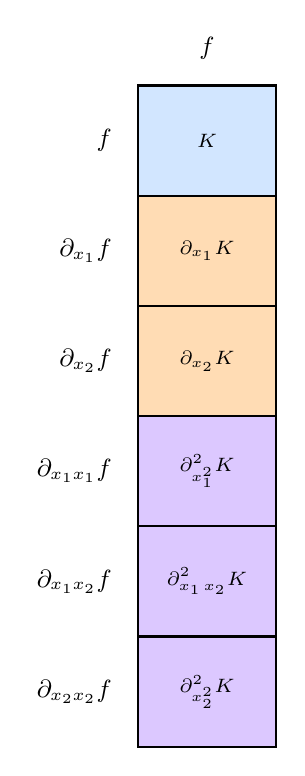
\begin{tikzpicture}
			\def\bw{1.75}
			\def\bh{1.4}

			% Reduced Sigma_12^H: 6x1, first column only
			\fill[ffblock] (0, 5*\bh) rectangle (\bw, 6*\bh);
			\fill[fdblock] (0, 4*\bh) rectangle (\bw, 5*\bh);
			\fill[fdblock] (0, 3*\bh) rectangle (\bw, 4*\bh);
			\fill[fhblock] (0, 2*\bh) rectangle (\bw, 3*\bh);
			\fill[fhblock] (0, 1*\bh) rectangle (\bw, 2*\bh);
			\fill[fhblock] (0, 0*\bh) rectangle (\bw, 1*\bh);
			
			\draw[black, thick] (0,0) rectangle (\bw, 6*\bh);
			\foreach \i in {1,2,3,4,5} {
				\draw[black, thick] (0, \i*\bh) -- (\bw, \i*\bh);
			}

			% --- cell labels ---
			\node[font=\scriptsize] at (0.5*\bw, 5.5*\bh) {$K$};
			\node[font=\scriptsize] at (0.5*\bw, 4.5*\bh) {$\partial_{x_1} K$};
			\node[font=\scriptsize] at (0.5*\bw, 3.5*\bh) {$\partial_{x_2} K$};
			\node[font=\scriptsize] at (0.5*\bw, 2.5*\bh) {$\partial^2_{x_1^2} K$};
			\node[font=\scriptsize] at (0.5*\bw, 1.5*\bh) {$\partial^2_{x_1\,x_2} K$};
			\node[font=\scriptsize] at (0.5*\bw, 0.5*\bh) {$\partial^2_{x_2^2} K$};

			\node[left=6pt, font=\small] at (0, 5.5*\bh) {$f$};
			\node[left=6pt, font=\small] at (0, 4.5*\bh) {$\partial_{x_1} f$};
			\node[left=6pt, font=\small] at (0, 3.5*\bh) {$\partial_{x_2} f$};
			\node[left=6pt, font=\small] at (0, 2.5*\bh) {$\partial_{x_1x_1} f$};
			\node[left=6pt, font=\small] at (0, 1.5*\bh) {$\partial_{x_1x_2} f$};
			\node[left=6pt, font=\small] at (0, 0.5*\bh) {$\partial_{x_2x_2} f$};

			\node[above=6pt, font=\small] at (0.5*\bw, 6*\bh) {$f$};

		\end{tikzpicture}
		\caption{Reduced $\boldsymbol{\Sigma}^{H}_{12}$}
	\end{subfigure}
	\caption{Full (left) and reduced (right) training-test covariance block $\boldsymbol{\Sigma}^{H}_{12}$ for a HEGP with $d=2$, when only function values are predicted at test locations. The reduced form retains only the first column of blocks, reducing from a $6n \times 6n_*$ matrix to a $6n \times n_*$ matrix.}
	\label{fig:hegp_s12_reduction}
\end{figure}
This simplification significantly reduces the computational cost of making predictions while still benefiting from derivative information during training. More generally, predictions of any subset of derivatives can be obtained by retaining only the corresponding block columns in $\boldsymbol{\Sigma}_{12}$ and the corresponding block rows and columns in $\boldsymbol{\Sigma}_{22}$, without modifying the training covariance $\boldsymbol{\Sigma}_{11}$.

For example, suppose we wish to predict $f(\mathbf{X}_*)$ and $\partial_{x_1} f(\mathbf{X}_*)$ at the test locations from a GEGP model with $d=2$. The cross-covariance block retains the $f$ and $\partial_{x_1'}$ columns, and the test covariance block retains the corresponding $2 \times 2$ block of rows and columns:
\begin{equation}
	\boldsymbol{\Sigma}_{12}^{G} \;\longrightarrow\;
	\begin{pmatrix}
		K & \partial_{x_1'} K \\
		\partial_{x_1} K & \partial^2_{x_1\,x_1'} K \\
		\partial_{x_2} K & \partial^2_{x_2\,x_1'} K
	\end{pmatrix}, \quad \text{and} \quad
	\boldsymbol{\Sigma}_{22}^{G} \;\longrightarrow\;
	\begin{pmatrix}
		K & \partial_{x_1'} K \\
		\partial_{x_1} K & \partial^2_{x_1\,x_1'} K
	\end{pmatrix}.
\end{equation}
Similarly, to predict $f(\mathbf{X}_*)$ and the gradient ($\partial_{x_1} f(\mathbf{X}_*)$ and $\partial_{x_2} f(\mathbf{X}_*)$) from a HEGP model with $d=2$, the cross-covariance retains the $f$, $\partial_{x_1'}$, and $\partial_{x_2'}$ columns, and the test covariance block retains the corresponding $3 \times 3$ block of rows and columns:
\begin{equation}
	\boldsymbol{\Sigma}_{12}^{H} \;\longrightarrow\;
	\begin{pmatrix}
		K & \partial_{x_1'} K & \partial_{x_2'} K \\
		\partial_{x_1} K & \partial^2_{x_1\,x_1'} K & \partial^2_{x_1\,x_2'} K \\
		\partial_{x_2} K & \partial^2_{x_2\,x_1'} K & \partial^2_{x_2\,x_2'} K \\
		\partial_{x_1^2} K & \partial^3_{x_1^2\,x_1'} K & \partial^3_{x_1^2\,x_2'} K \\
		\partial_{x_1\,x_2} K & \partial^3_{x_1\,x_2\,x_1'} K & \partial^3_{x_1\,x_2\,x_2'} K \\
		\partial_{x_2^2} K & \partial^3_{x_2^2\,x_1'} K & \partial^3_{x_2^2\,x_2'} K
	\end{pmatrix}, \quad \text{and} \quad
	\boldsymbol{\Sigma}_{22}^{H} \;\longrightarrow\;
	\begin{pmatrix}
		K & \partial_{x_1'} K & \partial_{x_2'} K \\
		\partial_{x_1} K & \partial^2_{x_1\,x_1'} K & \partial^2_{x_1\,x_2'} K \\
		\partial_{x_2} K & \partial^2_{x_2\,x_1'} K & \partial^2_{x_2\,x_2'} K
	\end{pmatrix}.
\end{equation}
The block structures for these two examples are illustrated in Figure~\ref{fig:subset_deriv_prediction}.
\begin{figure}[H]
	\centering
	%% --- (a) GEGP Sigma_12 ---
	\begin{subfigure}[t]{0.45\textwidth}
		\centering
		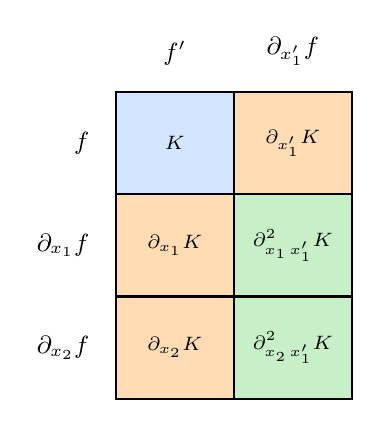
\begin{tikzpicture}
			\def\bw{1.5}
			\def\bh{1.3}
			% GEGP Sigma_12: 3x2 (f' and dx1' columns)
			% Column 1: f'
			\fill[ffblock] (0, 2*\bh) rectangle (\bw, 3*\bh);
			\fill[fdblock] (0, 1*\bh) rectangle (\bw, 2*\bh);
			\fill[fdblock] (0, 0)     rectangle (\bw, 1*\bh);
			% Column 2: dx1'
			\fill[fdblock] (\bw, 2*\bh) rectangle (2*\bw, 3*\bh);
			\fill[ddblock] (\bw, 1*\bh) rectangle (2*\bw, 2*\bh);
			\fill[ddblock] (\bw, 0)     rectangle (2*\bw, 1*\bh);

			\draw[black, thick] (0,0) rectangle (2*\bw, 3*\bh);
			\draw[black, thick] (0, \bh) -- (2*\bw, \bh);
			\draw[black, thick] (0, 2*\bh) -- (2*\bw, 2*\bh);
			\draw[black, thick] (\bw, 0) -- (\bw, 3*\bh);

			\node[font=\scriptsize] at (0.5*\bw, 2.5*\bh) {$K$};
			\node[font=\scriptsize] at (1.5*\bw, 2.5*\bh) {$\partial_{x_1'} K$};
			\node[font=\scriptsize] at (0.5*\bw, 1.5*\bh) {$\partial_{x_1} K$};
			\node[font=\scriptsize] at (1.5*\bw, 1.5*\bh) {$\partial^2_{x_1\,x_1'} K$};
			\node[font=\scriptsize] at (0.5*\bw, 0.5*\bh) {$\partial_{x_2} K$};
			\node[font=\scriptsize] at (1.5*\bw, 0.5*\bh) {$\partial^2_{x_2\,x_1'} K$};

			\node[left=6pt, font=\small] at (0, 2.5*\bh) {$f$};
			\node[left=6pt, font=\small] at (0, 1.5*\bh) {$\partial_{x_1} f$};
			\node[left=6pt, font=\small] at (0, 0.5*\bh) {$\partial_{x_2} f$};

			\node[above=6pt, font=\small] at (0.5*\bw, 3*\bh) {$f'$};
			\node[above=6pt, font=\small] at (1.5*\bw, 3*\bh) {$\partial_{x_1'} f$};

		\end{tikzpicture}
		\caption{GEGP $\boldsymbol{\Sigma}^G_{12}$}
	\end{subfigure}
	\hfill
	%% --- (b) GEGP Sigma_22 ---
	\begin{subfigure}[t]{0.45\textwidth}
		\centering
		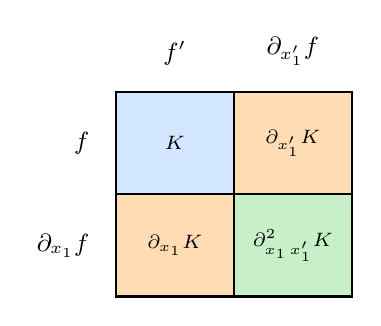
\begin{tikzpicture}
			\def\bw{1.5}
			\def\bh{1.3}
			% GEGP Sigma_22: 2x2 (f' and dx1' rows/columns)
			% Row f (top)
			\fill[ffblock] (0, \bh) rectangle (\bw, 2*\bh);
			\fill[fdblock] (\bw, \bh) rectangle (2*\bw, 2*\bh);
			% Row dx1
			\fill[fdblock] (0, 0) rectangle (\bw, \bh);
			\fill[ddblock] (\bw, 0) rectangle (2*\bw, \bh);

			\draw[black, thick] (0,0) rectangle (2*\bw, 2*\bh);
			\draw[black, thick] (0, \bh) -- (2*\bw, \bh);
			\draw[black, thick] (\bw, 0) -- (\bw, 2*\bh);

			\node[font=\scriptsize] at (0.5*\bw, 1.5*\bh) {$K$};
			\node[font=\scriptsize] at (1.5*\bw, 1.5*\bh) {$\partial_{x_1'} K$};
			\node[font=\scriptsize] at (0.5*\bw, 0.5*\bh) {$\partial_{x_1} K$};
			\node[font=\scriptsize] at (1.5*\bw, 0.5*\bh) {$\partial^2_{x_1\,x_1'} K$};

			\node[left=6pt, font=\small] at (0, 1.5*\bh) {$f$};
			\node[left=6pt, font=\small] at (0, 0.5*\bh) {$\partial_{x_1} f$};

			\node[above=6pt, font=\small] at (0.5*\bw, 2*\bh) {$f'$};
			\node[above=6pt, font=\small] at (1.5*\bw, 2*\bh) {$\partial_{x_1'} f$};

		\end{tikzpicture}
		\caption{GEGP $\boldsymbol{\Sigma}^G_{22}$}
	\end{subfigure}

	\vspace{12pt}

	%% --- (c) HEGP Sigma_12 ---
	\begin{subfigure}[t]{0.55\textwidth}
		\centering
		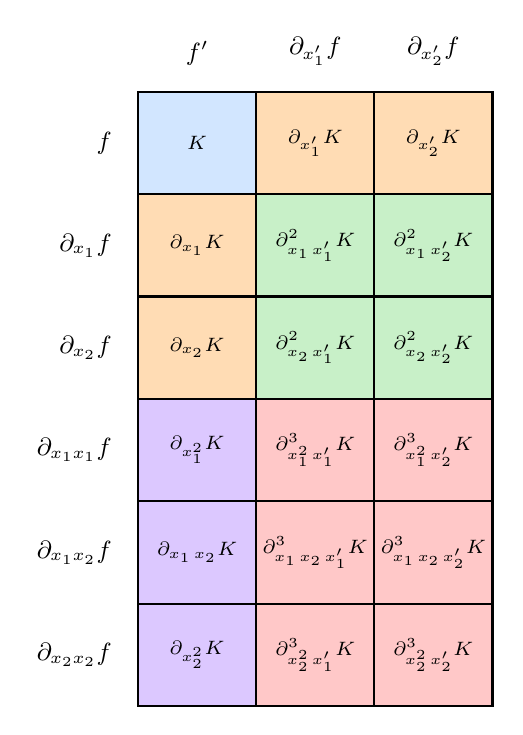
\begin{tikzpicture}
				\def\bw{1.5}
				\def\bh{1.3}
				% HEGP Sigma_12: 6x3 (f', dx1', dx2' columns)
				% Column 1: f'
				\fill[ffblock] (0, 5*\bh) rectangle (\bw, 6*\bh);
				\fill[fdblock] (0, 4*\bh) rectangle (\bw, 5*\bh);
				\fill[fdblock] (0, 3*\bh) rectangle (\bw, 4*\bh);
				\fill[fhblock] (0, 2*\bh) rectangle (\bw, 3*\bh);
				\fill[fhblock] (0, 1*\bh) rectangle (\bw, 2*\bh);
				\fill[fhblock] (0, 0)     rectangle (\bw, 1*\bh);
				% Column 2: dx1'
				\fill[fdblock] (\bw, 5*\bh) rectangle (2*\bw, 6*\bh);
				\fill[ddblock] (\bw, 4*\bh) rectangle (2*\bw, 5*\bh);
				\fill[ddblock] (\bw, 3*\bh) rectangle (2*\bw, 4*\bh);
				\fill[ghblock] (\bw, 2*\bh) rectangle (2*\bw, 3*\bh);
				\fill[ghblock] (\bw, 1*\bh) rectangle (2*\bw, 2*\bh);
				\fill[ghblock] (\bw, 0)     rectangle (2*\bw, 1*\bh);
				% Column 3: dx2'
				\fill[fdblock] (2*\bw, 5*\bh) rectangle (3*\bw, 6*\bh);
				\fill[ddblock] (2*\bw, 4*\bh) rectangle (3*\bw, 5*\bh);
				\fill[ddblock] (2*\bw, 3*\bh) rectangle (3*\bw, 4*\bh);
				\fill[ghblock] (2*\bw, 2*\bh) rectangle (3*\bw, 3*\bh);
				\fill[ghblock] (2*\bw, 1*\bh) rectangle (3*\bw, 2*\bh);
				\fill[ghblock] (2*\bw, 0)     rectangle (3*\bw, 1*\bh);

				\draw[black, thick] (0,0) rectangle (3*\bw, 6*\bh);
				\foreach \i in {1,2,3,4,5} {
					\draw[black, thick] (0, \i*\bh) -- (3*\bw, \i*\bh);
				}
				\draw[black, thick] (\bw, 0) -- (\bw, 6*\bh);
				\draw[black, thick] (2*\bw, 0) -- (2*\bw, 6*\bh);

				% Cell labels
				\node[font=\scriptsize] at (0.5*\bw, 5.5*\bh) {$K$};
				\node[font=\scriptsize] at (1.5*\bw, 5.5*\bh) {$\partial_{x_1'} K$};
				\node[font=\scriptsize] at (2.5*\bw, 5.5*\bh) {$\partial_{x_2'} K$};
				\node[font=\scriptsize] at (0.5*\bw, 4.5*\bh) {$\partial_{x_1} K$};
				\node[font=\scriptsize] at (1.5*\bw, 4.5*\bh) {$\partial^2_{x_1\,x_1'} K$};
				\node[font=\scriptsize] at (2.5*\bw, 4.5*\bh) {$\partial^2_{x_1\,x_2'} K$};
				\node[font=\scriptsize] at (0.5*\bw, 3.5*\bh) {$\partial_{x_2} K$};
				\node[font=\scriptsize] at (1.5*\bw, 3.5*\bh) {$\partial^2_{x_2\,x_1'} K$};
				\node[font=\scriptsize] at (2.5*\bw, 3.5*\bh) {$\partial^2_{x_2\,x_2'} K$};
				\node[font=\scriptsize] at (0.5*\bw, 2.5*\bh) {$\partial_{x_1^2} K$};
				\node[font=\scriptsize] at (1.5*\bw, 2.5*\bh) {$\partial^3_{x_1^2\,x_1'} K$};
				\node[font=\scriptsize] at (2.5*\bw, 2.5*\bh) {$\partial^3_{x_1^2\,x_2'} K$};
				\node[font=\scriptsize] at (0.5*\bw, 1.5*\bh) {$\partial_{x_1\,x_2} K$};
				\node[font=\scriptsize] at (1.5*\bw, 1.5*\bh) {$\partial^3_{x_1\,x_2\,x_1'} K$};
				\node[font=\scriptsize] at (2.5*\bw, 1.5*\bh) {$\partial^3_{x_1\,x_2\,x_2'} K$};
				\node[font=\scriptsize] at (0.5*\bw, 0.5*\bh) {$\partial_{x_2^2} K$};
				\node[font=\scriptsize] at (1.5*\bw, 0.5*\bh) {$\partial^3_{x_2^2\,x_1'} K$};
				\node[font=\scriptsize] at (2.5*\bw, 0.5*\bh) {$\partial^3_{x_2^2\,x_2'} K$};

				% Row labels
				\node[left=6pt, font=\small] at (0, 5.5*\bh) {$f$};
				\node[left=6pt, font=\small] at (0, 4.5*\bh) {$\partial_{x_1} f$};
				\node[left=6pt, font=\small] at (0, 3.5*\bh) {$\partial_{x_2} f$};
				\node[left=6pt, font=\small] at (0, 2.5*\bh) {$\partial_{x_1 x_1} f$};
				\node[left=6pt, font=\small] at (0, 1.5*\bh) {$\partial_{x_1 x_2} f$};
				\node[left=6pt, font=\small] at (0, 0.5*\bh) {$\partial_{x_2 x_2} f$};

				% Column headers
				\node[above=6pt, font=\small] at (0.5*\bw, 6*\bh) {$f'$};
				\node[above=6pt, font=\small] at (1.5*\bw, 6*\bh) {$\partial_{x_1'} f$};
				\node[above=6pt, font=\small] at (2.5*\bw, 6*\bh) {$\partial_{x_2'} f$};

		\end{tikzpicture}
		\caption{HEGP $\boldsymbol{\Sigma}^H_{12}$}
	\end{subfigure}
	\hfill
	%% --- (d) HEGP Sigma_22 ---
	\begin{subfigure}[t]{0.40\textwidth}
		\centering
		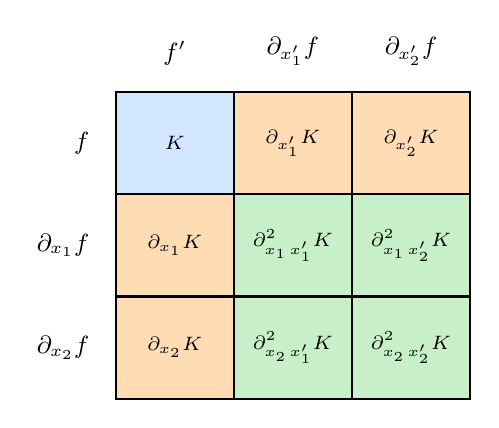
\begin{tikzpicture}
			\def\bw{1.5}
			\def\bh{1.3}
			% HEGP Sigma_22: 3x3
			% Row f (top)
			\fill[ffblock] (0, 2*\bh) rectangle (\bw, 3*\bh);
			\fill[fdblock] (\bw, 2*\bh) rectangle (2*\bw, 3*\bh);
			\fill[fdblock] (2*\bw, 2*\bh) rectangle (3*\bw, 3*\bh);
			% Row dx1
			\fill[fdblock] (0, \bh) rectangle (\bw, 2*\bh);
			\fill[ddblock] (\bw, \bh) rectangle (2*\bw, 2*\bh);
			\fill[ddblock] (2*\bw, \bh) rectangle (3*\bw, 2*\bh);
			% Row dx2
			\fill[fdblock] (0, 0) rectangle (\bw, \bh);
			\fill[ddblock] (\bw, 0) rectangle (2*\bw, \bh);
			\fill[ddblock] (2*\bw, 0) rectangle (3*\bw, \bh);

			\draw[black, thick] (0,0) rectangle (3*\bw, 3*\bh);
			\draw[black, thick] (0, \bh) -- (3*\bw, \bh);
			\draw[black, thick] (0, 2*\bh) -- (3*\bw, 2*\bh);
			\draw[black, thick] (\bw, 0) -- (\bw, 3*\bh);
			\draw[black, thick] (2*\bw, 0) -- (2*\bw, 3*\bh);

			\node[font=\scriptsize] at (0.5*\bw, 2.5*\bh) {$K$};
			\node[font=\scriptsize] at (1.5*\bw, 2.5*\bh) {$\partial_{x_1'} K$};
			\node[font=\scriptsize] at (2.5*\bw, 2.5*\bh) {$\partial_{x_2'} K$};
			\node[font=\scriptsize] at (0.5*\bw, 1.5*\bh) {$\partial_{x_1} K$};
			\node[font=\scriptsize] at (1.5*\bw, 1.5*\bh) {$\partial^2_{x_1\,x_1'} K$};
			\node[font=\scriptsize] at (2.5*\bw, 1.5*\bh) {$\partial^2_{x_1\,x_2'} K$};
			\node[font=\scriptsize] at (0.5*\bw, 0.5*\bh) {$\partial_{x_2} K$};
			\node[font=\scriptsize] at (1.5*\bw, 0.5*\bh) {$\partial^2_{x_2\,x_1'} K$};
			\node[font=\scriptsize] at (2.5*\bw, 0.5*\bh) {$\partial^2_{x_2\,x_2'} K$};

			\node[left=6pt, font=\small] at (0, 2.5*\bh) {$f$};
			\node[left=6pt, font=\small] at (0, 1.5*\bh) {$\partial_{x_1} f$};
			\node[left=6pt, font=\small] at (0, 0.5*\bh) {$\partial_{x_2} f$};

			\node[above=6pt, font=\small] at (0.5*\bw, 3*\bh) {$f'$};
			\node[above=6pt, font=\small] at (1.5*\bw, 3*\bh) {$\partial_{x_1'} f$};
			\node[above=6pt, font=\small] at (2.5*\bw, 3*\bh) {$\partial_{x_2'} f$};

		\end{tikzpicture}
		\caption{HEGP $\boldsymbol{\Sigma}^H_{22}$}
	\end{subfigure}
	\caption{Examples of selective derivative prediction for $d=2$. (a)--(b)~Predicting $f$ and $\partial_{x_1} f$ from a GEGP: $\boldsymbol{\Sigma}_{12}^G$ retains the $f$ and $\partial_{x_1'}$ block columns ($3n \times 2n_*$) and $\boldsymbol{\Sigma}_{22}^G$ reduces to a $2n_* \times 2n_*$ matrix. (c)--(d)~Predicting $f$ and the gradient from a HEGP: $\boldsymbol{\Sigma}_{12}^H$ retains the $f$, $\partial_{x_1'}$, and $\partial_{x_2'}$ block columns ($6n \times 3n_*$) and $\boldsymbol{\Sigma}_{22}^H$ reduces to a $3n_* \times 3n_*$ matrix.}
	\label{fig:subset_deriv_prediction}
\end{figure}

\subsection{Partial Gradient Enhanced Gaussian Processes}
\label{subsec:pgegp}
One approach to reducing computational cost selectively incorporates partial derivative information, using only a subset of available gradients rather than all $d$ derivatives~\cite{Ulaganathan2016-xq, Ulaganathan2014-yh}. The Partial Gradient-Enhanced GP (PGEGP), known in the literature as Partial Gradient-Enhanced Kriging (PGEK)~\cite{CHEN201915}, extends this concept by systematically identifying which gradients to include. PGEGP employs a two-step process: first, a feature selection technique, such as Mutual Information (MI), ranks the influence of each input variable on the output; second, an empirical evaluation rule determines the optimal number of gradients to include, balancing modeling efficiency and accuracy.

\subsubsection{Formulation}
\label{subsubsec:pgegp_formulation}

Suppose that feature selection identifies a subset of $m \leq d$ input variables $\mathbf{X}_A = \{x_{a_1}, \ldots, x_{a_m}\} \subseteq \{x_1, \ldots, x_d\}$ whose derivatives provide the best trade-off between accuracy and efficiency. For notational convenience, the equations below index these selected variables as $x_1, \ldots, x_m$. The formulation follows the structure of Section~\ref{subsec:derivative_gps}, but with a reduced observation vector. The observation vector $\mathbf{y}$ is augmented to include only the selected partial derivatives, forming $\mathbf{y}^{\text{PGEGP}}$. The test vector $\mathbf{y}^{\text{PGEGP}}_*$ need not mirror this structure; it can be extended to include derivatives of interest beyond those used in training (see Remark~2). By default, however, it includes the same selected derivatives:

\begin{equation}
	\label{eqn:pgegp_aug_vectors}
	\mathbf{y}^{\text{PGEGP}} = \begin{bmatrix} f(\mathbf{X}) \\ \partial_{x_1} f(\mathbf{X}) \\ \vdots \\ \partial_{x_m} f(\mathbf{X}) \end{bmatrix}, \quad
	\mathbf{y}^{\text{PGEGP}}_* = \begin{bmatrix} f(\mathbf{X}_*) \\ \partial_{x_1} f(\mathbf{X}_*) \\ \vdots \\ \partial_{x_m} f(\mathbf{X}_*) \end{bmatrix}.
\end{equation}

The joint distribution between the augmented training observations and test predictions remains multivariate Gaussian:

\begin{equation}
	\label{eqn:pgegp_joint_dist}
	\begin{pmatrix}
		\mathbf{y}^{\text{PGEGP}} \\
		\mathbf{y}^{\text{PGEGP}}_*
	\end{pmatrix}
	\sim \mathcal{N}\left(
	\mathbf{0},
	\begin{pmatrix}
		\boldsymbol{\Sigma}^{\text{PGEGP}}_{11} & \boldsymbol{\Sigma}^{\text{PGEGP}}_{12} \\
		\boldsymbol{\Sigma}^{\text{PGEGP}}_{21} & \boldsymbol{\Sigma}^{\text{PGEGP}}_{22}
	\end{pmatrix}
	\right).
\end{equation}

The training covariance block $\boldsymbol{\Sigma}^{\text{PGEGP}}_{11}$ is an $n(m+1) \times n(m+1)$ matrix constructed using only the selected derivatives:

\begin{equation}
	\label{eqn:pgegp_S11}
	\boldsymbol{\Sigma}^{\text{PGEGP}}_{11} =
	\begin{pmatrix}
		K & \partial_{\mathbf{X}_A'} K \\
		\partial_{\mathbf{X}_A} K & \partial^2_{\mathbf{X}_A\,\mathbf{X}_A'} K
	\end{pmatrix},
\end{equation}
where $\mathbf{X}_A$ denotes the subset of selected input dimensions. The cross-covariance blocks $\boldsymbol{\Sigma}^{\text{PGEGP}}_{12}$ and $\boldsymbol{\Sigma}^{\text{PGEGP}}_{22}$ are constructed analogously. The posterior predictive distribution for the augmented test vector $\mathbf{y}^{\text{PGEGP}}_*$ is given by:
\begin{equation}
	\label{eqn:pgegp_posterior}
	\begin{split}
		\boldsymbol{\mu}_{*}^{\text{PGEGP}} &= \boldsymbol{\Sigma}^{\text{PGEGP}}_{21} \left(\boldsymbol{\Sigma}^{\text{PGEGP}}_{11}\right)^{-1} \mathbf{y}^{\text{PGEGP}} \\
		\boldsymbol{\Sigma}_{*}^{\text{PGEGP}} &= \boldsymbol{\Sigma}^{\text{PGEGP}}_{22} - \boldsymbol{\Sigma}^{\text{PGEGP}}_{21} \left(\boldsymbol{\Sigma}^{\text{PGEGP}}_{11}\right)^{-1} \boldsymbol{\Sigma}^{\text{PGEGP}}_{12}
	\end{split}
\end{equation}
The posterior mean $\boldsymbol{\mu}_{*}^{\text{PGEGP}}$ provides predictions for function values and the selected derivatives in $\mathbf{X}_A$, while $\boldsymbol{\Sigma}_{*}^{\text{PGEGP}}$ provides their uncertainty. The kernel hyperparameters $\boldsymbol{\psi}$ are determined by maximizing the log marginal likelihood of the augmented observations:
\begin{equation}
	\label{eqn:pgegp_mll}
	\resizebox{0.92\textwidth}{!}{$\displaystyle
	\log p(\mathbf{y}^{\text{PGEGP}}|\mathbf{X}, \boldsymbol{\psi}) = -\frac{1}{2} \left(\mathbf{y}^{\text{PGEGP}}\right)^\top \left(\boldsymbol{\Sigma}^{\text{PGEGP}}_{11}\right)^{-1} \mathbf{y}^{\text{PGEGP}} - \frac{1}{2}\log|\boldsymbol{\Sigma}^{\text{PGEGP}}_{11}| - \frac{n(m+1)}{2}\log 2\pi
	$}
\end{equation}

To make this concrete, consider the case $d = 2$ with only the derivative with respect to $x_2$ selected ($m = 1$, $\mathbf{X}_A = \{x_2\}$). The augmented training and test vectors take the form:
\begin{equation}
	\label{eqn:pgegp_aug_vectors_2d}
	\mathbf{y}^{\text{PGEGP}} = \begin{bmatrix} f(\mathbf{X}) \\ \partial_{x_2} f(\mathbf{X}) \end{bmatrix}, \quad
	\mathbf{y}^{\text{PGEGP}}_* = \begin{bmatrix} f(\mathbf{X}_*) \\ \partial_{x_2} f(\mathbf{X}_*) \end{bmatrix},
\end{equation}
and the training covariance block reduces to a $2n \times 2n$ matrix:
\begin{equation}
	\label{eqn:pgegp_S11_2d}
	\boldsymbol{\Sigma}^{\text{PGEGP}}_{11} =
	\begin{pmatrix}
		K & \partial_{x_2'} K \\[8pt]
		\partial_{x_2} K & \partial^2_{x_2\,x_2'} K
	\end{pmatrix}.
\end{equation}
Figure~\ref{fig:pgegp_structure_2d} illustrates the reduction from the full GEGP structure to PGEGP for this example. The excluded $x_1$-derivative entries are shown in black; arrows indicate how removing these entries yields the reduced PGEGP training vector and covariance matrix.
\begin{figure}[htbp]
	\centering

	% === (a) Training vector reduction ===
	\begin{subfigure}[b]{\textwidth}
		\centering
		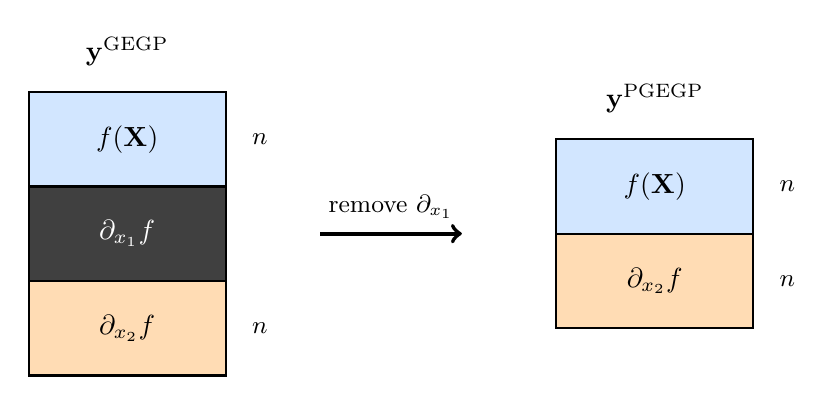
\begin{tikzpicture}
			\def\bw{2.5}
			\def\bh{1.2}

			% --- Left: GEGP vector (3 blocks) ---
			\fill[ffblock]  (0, 2*\bh) rectangle (\bw, 3*\bh);
			\fill[black!75] (0, 1*\bh) rectangle (\bw, 2*\bh);
			\fill[fdblock]  (0, 0)     rectangle (\bw, 1*\bh);

			\draw[black, thick] (0, 0) rectangle (\bw, 3*\bh);
			\draw[black, thick] (0, \bh)   -- (\bw, \bh);
			\draw[black, thick] (0, 2*\bh) -- (\bw, 2*\bh);

			\node at (0.5*\bw, 2.5*\bh) {$f(\mathbf{X})$};
			\node[text=white] at (0.5*\bw, 1.5*\bh) {$\partial_{x_1} f$};
			\node at (0.5*\bw, 0.5*\bh) {$\partial_{x_2} f$};

			\node[right=6pt, font=\small] at (\bw, 2.5*\bh) {$n$};
			\node[right=6pt, font=\small] at (\bw, 0.5*\bh) {$n$};

			\node[above=6pt, font=\normalsize] at (0.5*\bw, 3*\bh) {$\mathbf{y}^{\text{GEGP}}$};

			% --- Arrow ---
			\draw[->, line width=1.5pt] (\bw+1.2, 1.5*\bh) -- (\bw+3.0, 1.5*\bh);
			\node[above=2pt, font=\small] at (\bw+2.1, 1.5*\bh) {remove $\partial_{x_1}$};

			% --- Right: PGEGP vector (2 blocks, vertically centered) ---
			\pgfmathsetmacro{\rx}{\bw+4.2}
			\fill[ffblock] (\rx, 1.5*\bh) rectangle (\rx+\bw, 2.5*\bh);
			\fill[fdblock] (\rx, 0.5*\bh) rectangle (\rx+\bw, 1.5*\bh);

			\draw[black, thick] (\rx, 0.5*\bh) rectangle (\rx+\bw, 2.5*\bh);
			\draw[black, thick] (\rx, 1.5*\bh) -- (\rx+\bw, 1.5*\bh);

			\node at (\rx+0.5*\bw, 2.0*\bh) {$f(\mathbf{X})$};
			\node at (\rx+0.5*\bw, 1.0*\bh) {$\partial_{x_2} f$};

			\node[right=6pt, font=\small] at (\rx+\bw, 2.0*\bh) {$n$};
			\node[right=6pt, font=\small] at (\rx+\bw, 1.0*\bh) {$n$};

			\node[above=6pt, font=\normalsize] at (\rx+0.5*\bw, 2.5*\bh) {$\mathbf{y}^{\text{PGEGP}}$};
		\end{tikzpicture}
		\caption{Training vector reduction: the excluded $x_1$-derivative entries (black) are removed, reducing $\mathbf{y}^{\text{GEGP}}$ ($3n$ entries) to $\mathbf{y}^{\text{PGEGP}}$ ($2n$ entries).}
		\label{fig:pgegp_vector_reduction}
	\end{subfigure}

	\vspace{14pt}

	% === (b) Covariance matrix reduction ===
	\begin{subfigure}[b]{\textwidth}
		\centering
		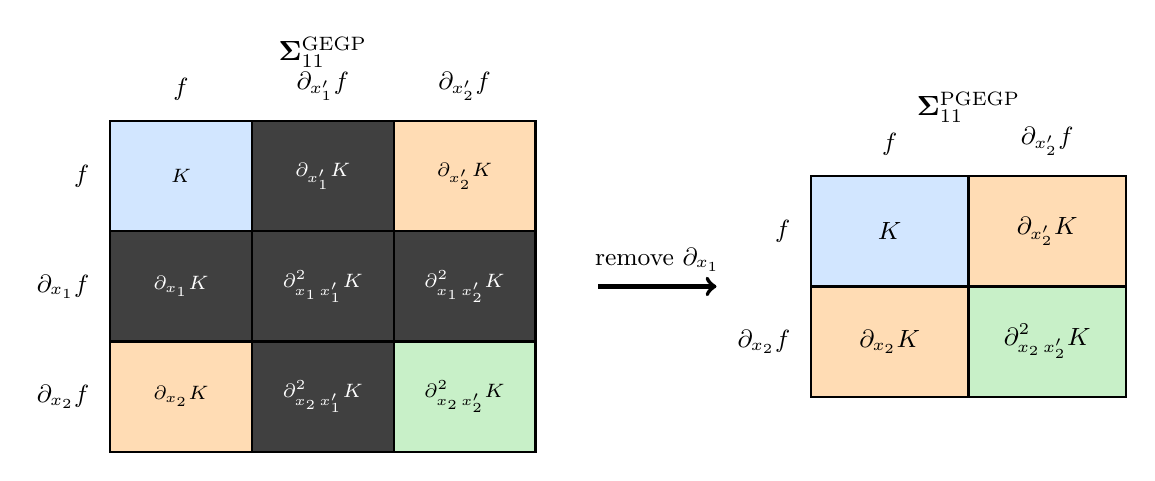
\begin{tikzpicture}
			\def\bw{1.8}
			\def\bh{1.4}
			\def\rbw{2.0}

			% --- Left: GEGP 3x3 matrix with blackout ---
			% Kept blocks
			\fill[ffblock] (0,      2*\bh) rectangle (1*\bw, 3*\bh);
			\fill[fdblock] (2*\bw,  2*\bh) rectangle (3*\bw, 3*\bh);
			\fill[fdblock] (0,      0)     rectangle (1*\bw, 1*\bh);
			\fill[ddblock] (2*\bw,  0)     rectangle (3*\bw, 1*\bh);

			% Excluded blocks (x_1 row and column)
			\fill[black!75] (1*\bw, 2*\bh) rectangle (2*\bw, 3*\bh);
			\fill[black!75] (0,     1*\bh) rectangle (1*\bw, 2*\bh);
			\fill[black!75] (1*\bw, 1*\bh) rectangle (2*\bw, 2*\bh);
			\fill[black!75] (2*\bw, 1*\bh) rectangle (3*\bw, 2*\bh);
			\fill[black!75] (1*\bw, 0)     rectangle (2*\bw, 1*\bh);

			% Grid
			\draw[black, thick] (0,0) rectangle (3*\bw, 3*\bh);
			\draw[black, thick] (1*\bw, 0) -- (1*\bw, 3*\bh);
			\draw[black, thick] (2*\bw, 0) -- (2*\bw, 3*\bh);
			\draw[black, thick] (0, 1*\bh) -- (3*\bw, 1*\bh);
			\draw[black, thick] (0, 2*\bh) -- (3*\bw, 2*\bh);

			% Cell labels for kept blocks
			\node[font=\scriptsize] at (0.5*\bw, 2.5*\bh) {$K$};
			\node[font=\scriptsize] at (2.5*\bw, 2.5*\bh) {$\partial_{x_2'} K$};
			\node[font=\scriptsize] at (0.5*\bw, 0.5*\bh) {$\partial_{x_2} K$};
			\node[font=\scriptsize] at (2.5*\bw, 0.5*\bh) {$\partial^2_{x_2\,x_2'} K$};

			% Cell labels for excluded blocks (white text)
			\node[font=\scriptsize, text=white] at (1.5*\bw, 2.5*\bh) {$\partial_{x_1'} K$};
			\node[font=\scriptsize, text=white] at (0.5*\bw, 1.5*\bh) {$\partial_{x_1} K$};
			\node[font=\scriptsize, text=white] at (1.5*\bw, 1.5*\bh) {$\partial^2_{x_1\,x_1'} K$};
			\node[font=\scriptsize, text=white] at (2.5*\bw, 1.5*\bh) {$\partial^2_{x_1\,x_2'} K$};
			\node[font=\scriptsize, text=white] at (1.5*\bw, 0.5*\bh) {$\partial^2_{x_2\,x_1'} K$};

			% Row/column headers
			\node[left=4pt, font=\small] at (0, 2.5*\bh) {$f$};
			\node[left=4pt, font=\small] at (0, 1.5*\bh) {$\partial_{x_1} f$};
			\node[left=4pt, font=\small] at (0, 0.5*\bh) {$\partial_{x_2} f$};

			\node[above=4pt, font=\small] at (0.5*\bw, 3*\bh) {$f$};
			\node[above=4pt, font=\small] at (1.5*\bw, 3*\bh) {$\partial_{x_1'} f$};
			\node[above=4pt, font=\small] at (2.5*\bw, 3*\bh) {$\partial_{x_2'} f$};

			% Matrix label
			\node[above=16pt, font=\normalsize] at (1.5*\bw, 3*\bh) {$\boldsymbol{\Sigma}_{11}^{\text{GEGP}}$};

			% --- Arrow ---
			\pgfmathsetmacro{\arrowstart}{3*\bw+0.8}
			\pgfmathsetmacro{\arrowend}{3*\bw+2.3}
			\pgfmathsetmacro{\arrowmid}{(\arrowstart+\arrowend)/2}
			\draw[->, line width=1.5pt] (\arrowstart, 1.5*\bh) -- (\arrowend, 1.5*\bh);
			\node[above=2pt, font=\small] at (\arrowmid, 1.5*\bh) {remove $\partial_{x_1}$};

			% --- Right: PGEGP 2x2 matrix (vertically centered) ---
			\pgfmathsetmacro{\rx}{3*\bw+3.5}

			\fill[ffblock] (\rx,      1.5*\bh) rectangle (\rx+\rbw, 2.5*\bh);
			\fill[fdblock] (\rx+\rbw, 1.5*\bh) rectangle (\rx+2*\rbw, 2.5*\bh);
			\fill[fdblock] (\rx,      0.5*\bh) rectangle (\rx+\rbw, 1.5*\bh);
			\fill[ddblock] (\rx+\rbw, 0.5*\bh) rectangle (\rx+2*\rbw, 1.5*\bh);

			% Grid
			\draw[black, thick] (\rx, 0.5*\bh) rectangle (\rx+2*\rbw, 2.5*\bh);
			\draw[black, thick] (\rx+\rbw, 0.5*\bh) -- (\rx+\rbw, 2.5*\bh);
			\draw[black, thick] (\rx, 1.5*\bh) -- (\rx+2*\rbw, 1.5*\bh);

			% Cell labels
			\node[font=\small] at (\rx+0.5*\rbw, 2.0*\bh) {$K$};
			\node[font=\small] at (\rx+1.5*\rbw, 2.0*\bh) {$\partial_{x_2'} K$};
			\node[font=\small] at (\rx+0.5*\rbw, 1.0*\bh) {$\partial_{x_2} K$};
			\node[font=\small] at (\rx+1.5*\rbw, 1.0*\bh) {$\partial^2_{x_2\,x_2'} K$};

			% Row/column headers
			\node[left=4pt, font=\small] at (\rx, 2.0*\bh) {$f$};
			\node[left=4pt, font=\small] at (\rx, 1.0*\bh) {$\partial_{x_2} f$};

			\node[above=4pt, font=\small] at (\rx+0.5*\rbw, 2.5*\bh) {$f$};
			\node[above=4pt, font=\small] at (\rx+1.5*\rbw, 2.5*\bh) {$\partial_{x_2'} f$};

			% Matrix label
			\node[above=16pt, font=\normalsize] at (\rx+\rbw, 2.5*\bh) {$\boldsymbol{\Sigma}_{11}^{\text{PGEGP}}$};
		\end{tikzpicture}
		\caption{Covariance matrix reduction: the excluded $x_1$-derivative rows and columns (black) are removed, reducing $\boldsymbol{\Sigma}_{11}^{\text{GEGP}}$ ($3n \times 3n$) to $\boldsymbol{\Sigma}_{11}^{\text{PGEGP}}$ ($2n \times 2n$).}
		\label{fig:pgegp_cov_reduction}
	\end{subfigure}

	\vspace{8pt}
	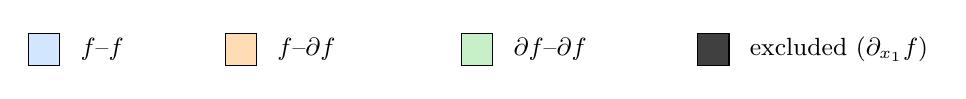
\begin{tikzpicture}
		\fill[ffblock] (0,0) rectangle (0.4, 0.4);
		\draw[black] (0,0) rectangle (0.4, 0.4);
		\node[right=4pt, font=\small] at (0.4, 0.2) {$f$--$f$};

		\fill[fdblock] (2.5,0) rectangle (2.9, 0.4);
		\draw[black] (2.5,0) rectangle (2.9, 0.4);
		\node[right=4pt, font=\small] at (2.9, 0.2) {$f$--$\partial f$};

		\fill[ddblock] (5.5,0) rectangle (5.9, 0.4);
		\draw[black] (5.5,0) rectangle (5.9, 0.4);
		\node[right=4pt, font=\small] at (5.9, 0.2) {$\partial f$--$\partial f$};

		\fill[black!75] (8.5,0) rectangle (8.9, 0.4);
		\draw[black] (8.5,0) rectangle (8.9, 0.4);
		\node[right=4pt, font=\small] at (8.9, 0.2) {excluded ($\partial_{x_1} f$)};
	\end{tikzpicture}

	\caption{PGEGP reduction for $d=2$ with only the $x_2$ partial derivative retained ($m=1$, $\mathbf{X}_A = \{x_2\}$). Left panels show the full GEGP structure with excluded $x_1$-derivative entries in black; right panels show the resulting PGEGP structure after removal. The observation vector reduces from $3n$ to $2n$ entries, and the training covariance matrix from $3n \times 3n$ to $2n \times 2n$.}
	\label{fig:pgegp_structure_2d}
\end{figure}

\paragraph{Numerical example.}
Using the same test function and training grid, the PGEGP includes only $\partial f / \partial x_1$ at all training points, discarding $\partial f / \partial x_2$ entirely. Figure~\ref{fig:pgegp_example} shows that the prediction of $f$ and $\partial f / \partial x_1$ remains reasonable, while the prediction of $\partial f / \partial x_2$---which was not included in training---is noticeably less accurate. This illustrates the trade-off inherent in PGEGP: computational savings from reduced matrix size come at the cost of diminished prediction quality for the excluded derivative directions. Nevertheless, the GP can still produce non-trivial predictions for unobserved derivatives through the cross-covariance structure of the kernel.

\begin{figure}[H]
	\centering
	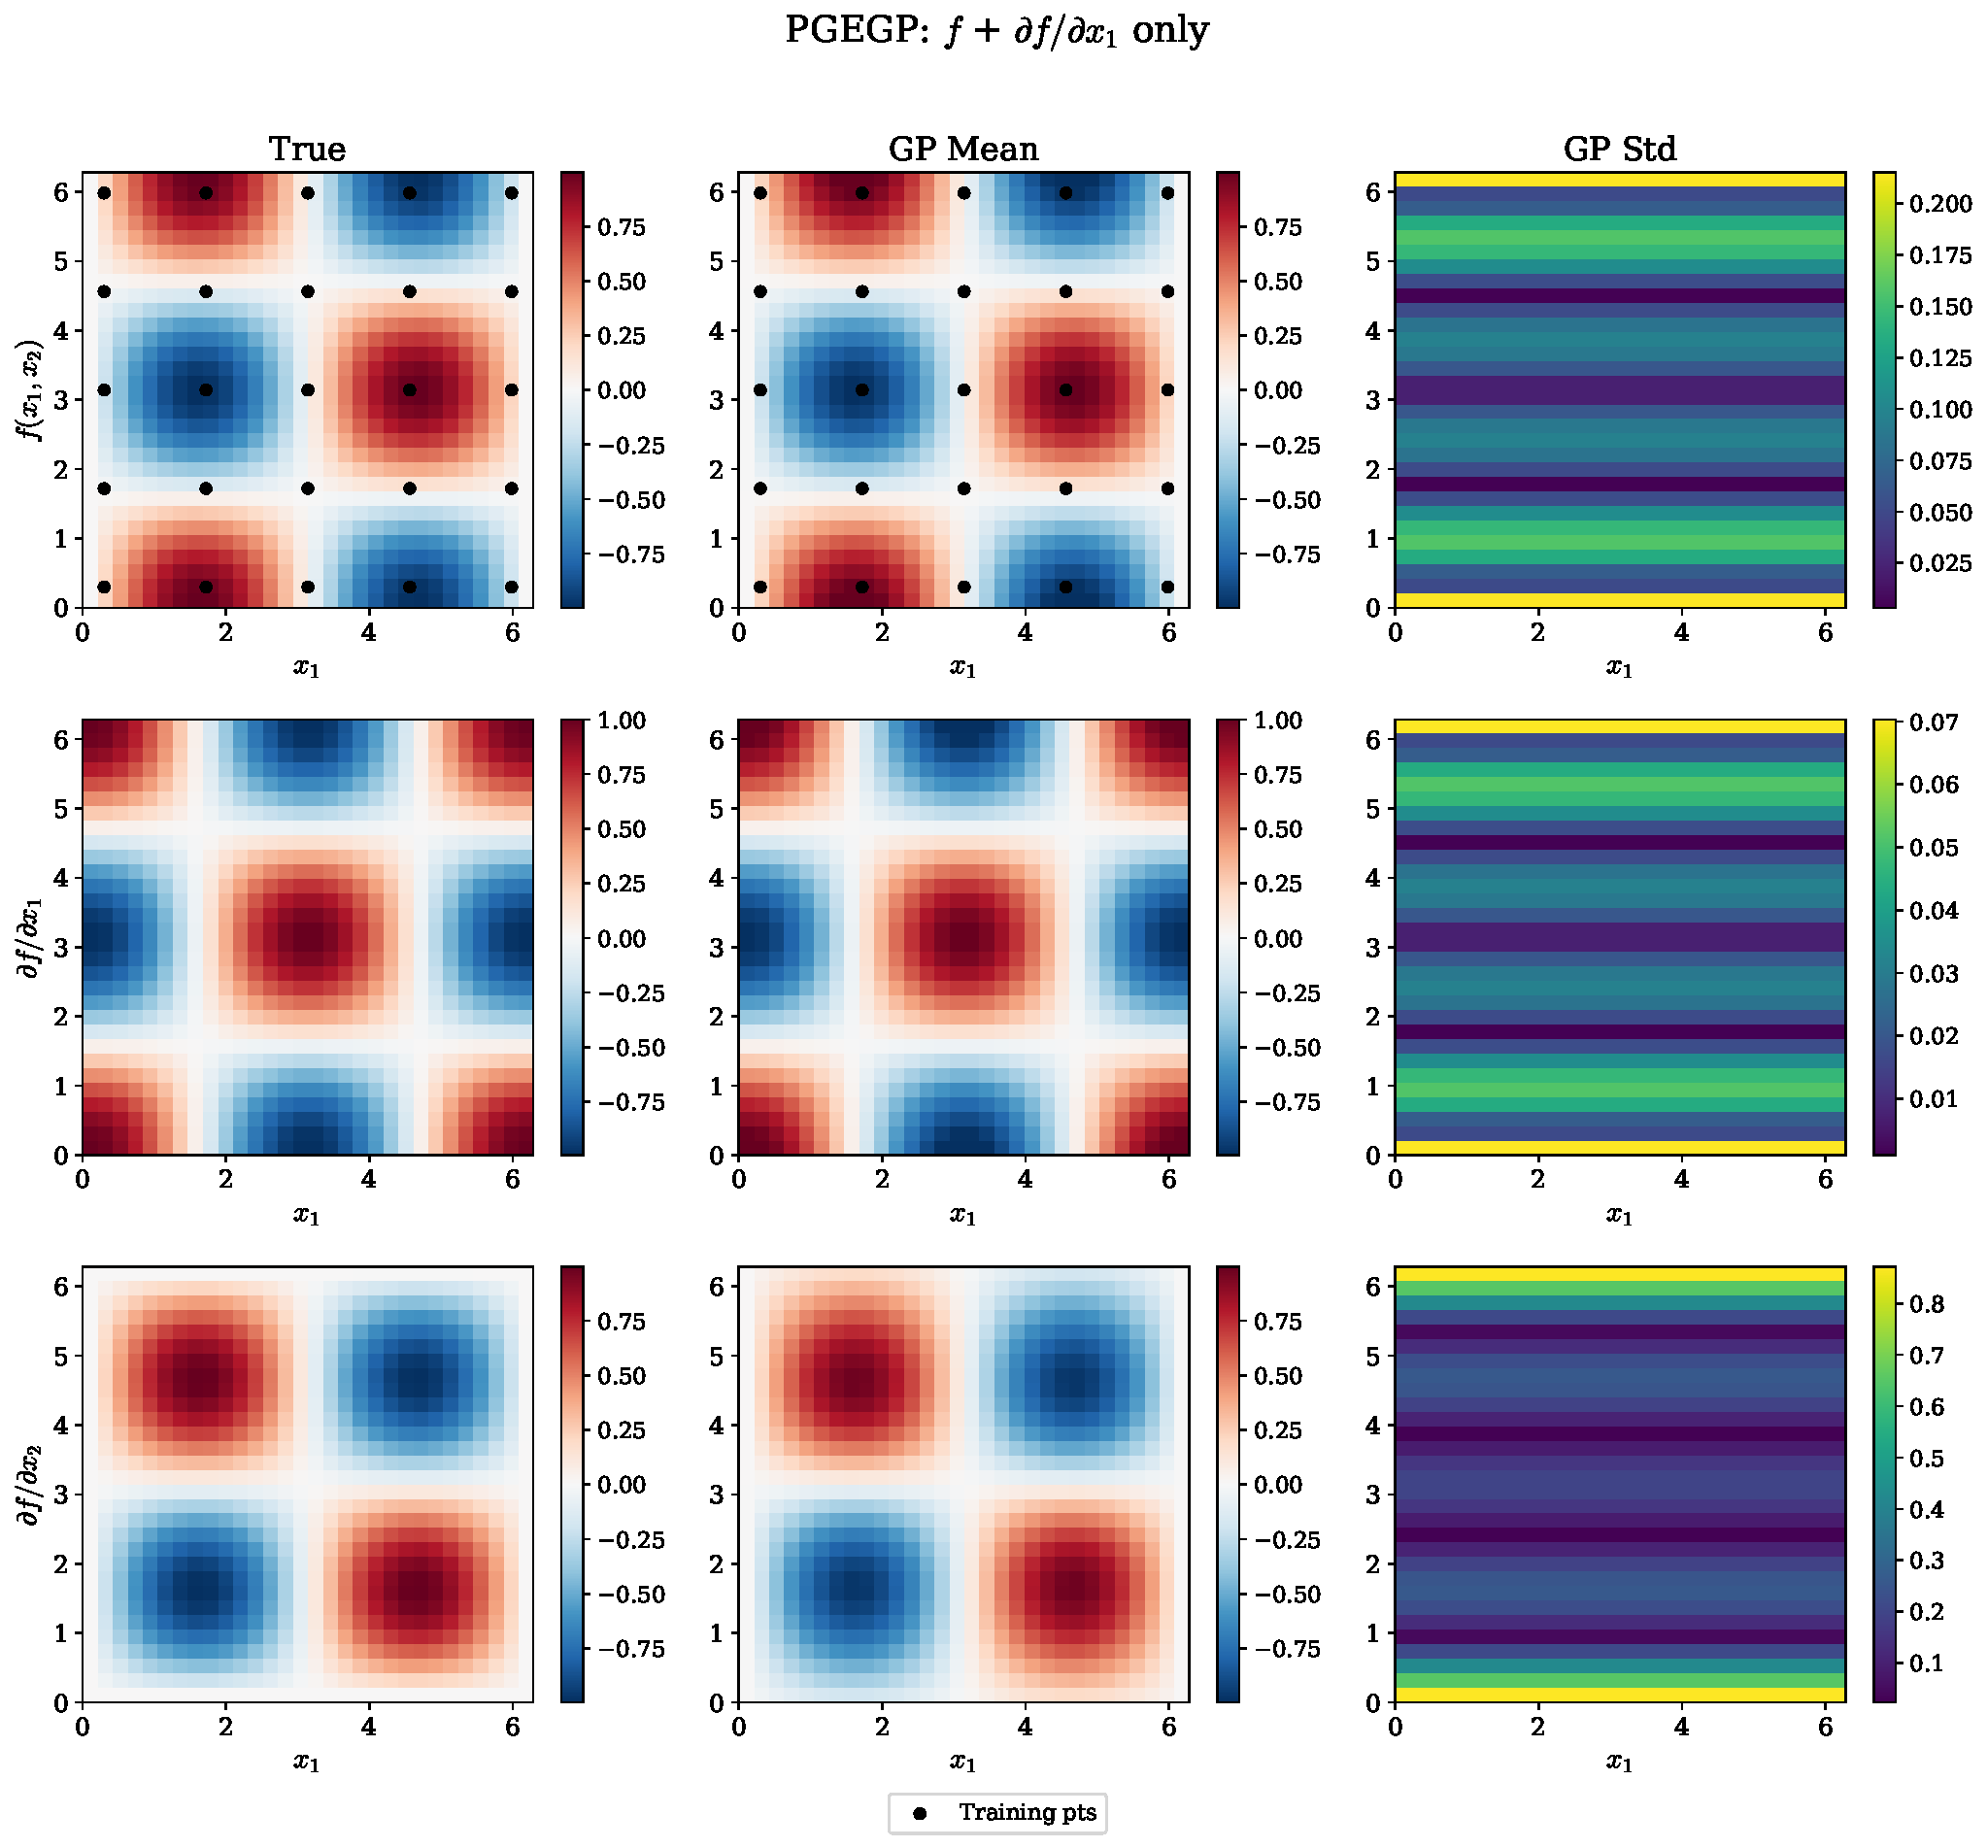
\includegraphics[width=\textwidth]{pgegp_example.pdf}
	\caption{PGEGP example on $f(x_1, x_2) = \sin(x_1)\cos(x_2)$ with $n = 25$ training points and only $\partial f / \partial x_1$ observed. Rows show $f$, $\partial f / \partial x_1$, and $\partial f / \partial x_2$; columns show the true function, GP posterior mean, and posterior standard deviation. The unobserved derivative $\partial f / \partial x_2$ shows higher predictive uncertainty and error compared to the GEGP (Figure~\ref{fig:gegp_example}).}
	\label{fig:pgegp_example}
\end{figure}

\subsubsection{Selective Derivative Predictions at Test Locations}
\label{subsubsec:pgegp_selective_pred}

The same principles for selective derivative predictions described in Section~\ref{subsec:selective_deriv_pred} apply to the PGEGP: predictions of any subset of function values and partial derivatives at test locations can be obtained by retaining the corresponding block columns in $\boldsymbol{\Sigma}_{12}$ and the corresponding block rows and columns in $\boldsymbol{\Sigma}_{22}$, without modifying $\boldsymbol{\Sigma}_{11}$.

As in the GEGP case, when only function values are required at test locations the training-test and test-test covariance blocks simplify. For the $d=2$, $\mathbf{X}_A = \{x_2\}$ example, the full training-test block is
\begin{equation}
	\boldsymbol{\Sigma}_{12}^{\text{PGEGP}} =
	\begin{pmatrix}
		K & \partial_{x_{2*}'} K \\[8pt]
		\partial_{x_2} K & \partial^2_{x_2\,x_{2*}'} K
	\end{pmatrix},
\end{equation}
When only $f(\mathbf{X}_*)$ is needed, the training-test and test-test covariance blocks reduce to
\begin{equation}
	\boldsymbol{\Sigma}_{12}^{\text{PGEGP}} \;\longrightarrow\;
	\begin{pmatrix}
		K \\[12pt]
		\partial_{x_2} K
	\end{pmatrix}, \quad \text{and} \quad
	\boldsymbol{\Sigma}_{22}^{\text{PGEGP}} \;\longrightarrow\; K.
\end{equation}
The block structure of both the full and reduced forms is illustrated in Figure~\ref{fig:pgegp_s12_reduction}.
\begin{figure}[htbp]
	\centering
	\begin{subfigure}[t]{0.45\textwidth}
		\centering
		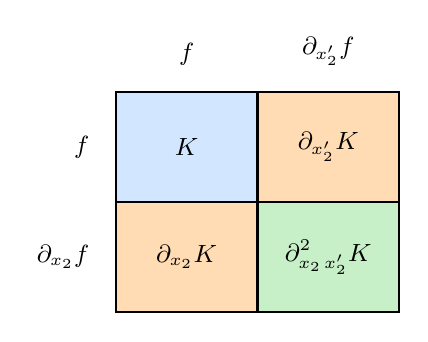
\begin{tikzpicture}
			\def\bw{1.8}
			\def\bh{1.4}

			% Full Sigma_12^PGEGP: 2x2
			\fill[ffblock] (0,     \bh) rectangle (\bw,   2*\bh);
			\fill[fdblock] (\bw,   \bh) rectangle (2*\bw, 2*\bh);
			\fill[fdblock] (0,     0)   rectangle (\bw,   \bh);
			\fill[ddblock] (\bw,   0)   rectangle (2*\bw, \bh);

			\draw[black, thick] (0,0) rectangle (2*\bw, 2*\bh);
			\draw[black, thick] (\bw, 0) -- (\bw, 2*\bh);
			\draw[black, thick] (0, \bh) -- (2*\bw, \bh);

			\node[font=\small] at (0.5*\bw, 1.5*\bh) {$K$};
			\node[font=\small] at (1.5*\bw, 1.5*\bh) {$\partial_{x_2'} K$};
			\node[font=\small] at (0.5*\bw, 0.5*\bh) {$\partial_{x_2} K$};
			\node[font=\small] at (1.5*\bw, 0.5*\bh) {$\partial^2_{x_2\,x_2'} K$};

			\node[left=6pt, font=\small] at (0, 1.5*\bh) {$f$};
			\node[left=6pt, font=\small] at (0, 0.5*\bh) {$\partial_{x_2} f$};

			\node[above=6pt, font=\small] at (0.5*\bw, 2*\bh) {$f$};
			\node[above=6pt, font=\small] at (1.5*\bw, 2*\bh) {$\partial_{x_2'} f$};
		\end{tikzpicture}
		\caption{Full $\boldsymbol{\Sigma}^{\text{PGEGP}}_{12}$}
		\label{fig:pgegp_s12_full}
	\end{subfigure}
	\hfill
	\begin{subfigure}[t]{0.45\textwidth}
		\centering
		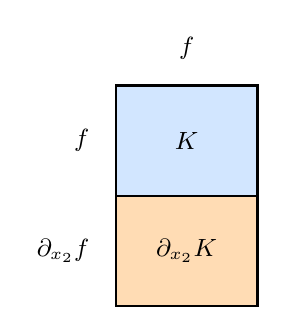
\begin{tikzpicture}
			\def\bw{1.8}
			\def\bh{1.4}

			% Reduced Sigma_12^PGEGP: 2x1
			\fill[ffblock] (0, \bh) rectangle (\bw, 2*\bh);
			\fill[fdblock] (0, 0)   rectangle (\bw, \bh);

			\draw[black, thick] (0,0) rectangle (\bw, 2*\bh);
			\draw[black, thick] (0, \bh) -- (\bw, \bh);

			\node[font=\small] at (0.5*\bw, 1.5*\bh) {$K$};
			\node[font=\small] at (0.5*\bw, 0.5*\bh) {$\partial_{x_2} K$};

			\node[left=6pt, font=\small] at (0, 1.5*\bh) {$f$};
			\node[left=6pt, font=\small] at (0, 0.5*\bh) {$\partial_{x_2} f$};

			\node[above=6pt, font=\small] at (0.5*\bw, 2*\bh) {$f$};

		\end{tikzpicture}
		\caption{Reduced $\boldsymbol{\Sigma}^{\text{PGEGP}}_{12}$}
		\label{fig:pgegp_s12_reduced}
	\end{subfigure}
	\caption{Full (left) and reduced (right) training-test covariance block $\boldsymbol{\Sigma}^{\text{PGEGP}}_{12}$ for a PGEGP with $d=2$ and $\mathbf{X}_A = \{x_2\}$, when only function values are predicted at test locations. The reduced form retains only the first column of blocks, reducing from a $2n \times 2n_*$ matrix to a $2n \times n_*$ matrix.}
	\label{fig:pgegp_s12_reduction}
\end{figure}

Although the PGEGP trains on only a subset of derivatives, it can still predict derivatives with respect to variables in $\mathbf{X}_B$ at test locations. The augmented test vector $\mathbf{y}^{\text{PGEGP}}_*$ is formed to include the derivatives of interest, and the covariance blocks $\boldsymbol{\Sigma}_{12}^{\text{PGEGP}}$ and $\boldsymbol{\Sigma}_{22}^{\text{PGEGP}}$ are extended accordingly, while $\boldsymbol{\Sigma}_{11}^{\text{PGEGP}}$ remains unchanged.

For the $d=2$, $\mathbf{X}_A = \{x_2\}$ example, suppose we wish to predict both $\partial_{x_1} f$ and $\partial_{x_2} f$ (in addition to $f$) at the test locations $\mathbf{X}_*$, even though only $x_2$ derivatives were included in training. The augmented test vector becomes
\begin{equation}
	\mathbf{y}^{\text{PGEGP}}_* = \begin{bmatrix} f(\mathbf{X}_*) \\ \partial_{x_1} f(\mathbf{X}_*) \\ \partial_{x_2} f(\mathbf{X}_*) \end{bmatrix},
\end{equation}
and the training-test covariance block is extended to
\begin{equation}
	\boldsymbol{\Sigma}_{12}^{\text{PGEGP}} =
	\begin{pmatrix}
		K & \partial_{x_{1*}'} K & \partial_{x_{2*}'} K \\[8pt]
		\partial_{x_2} K & \partial^2_{x_2\,x_{1*}'} K & \partial^2_{x_2\,x_{2*}'} K
	\end{pmatrix},
\end{equation}
and the test covariance block becomes the full $3n_* \times 3n_*$ matrix
\begin{equation}
	\boldsymbol{\Sigma}_{22}^{\text{PGEGP}} =
	\begin{pmatrix}
		K & \partial_{x_{1*}'} K & \partial_{x_{2*}'} K \\[8pt]
		\partial_{x_{1*}} K & \partial^2_{x_{1*}\,x_{1*}'} K & \partial^2_{x_{1*}\,x_{2*}'} K \\[8pt]
		\partial_{x_{2*}} K & \partial^2_{x_{2*}\,x_{1*}'} K & \partial^2_{x_{2*}\,x_{2*}'} K
	\end{pmatrix}.
\end{equation}
Note that the training covariance $\boldsymbol{\Sigma}_{11}^{\text{PGEGP}}$ remains $2n \times 2n$ — only the test-side blocks are extended. The resulting $\boldsymbol{\Sigma}_{12}$ is $2n \times 3n_*$ and $\boldsymbol{\Sigma}_{22}$ is $3n_* \times 3n_*$, recovering the full GEGP prediction structure on the test side while retaining the computational savings of the reduced training covariance. The block structure of the extended forms is illustrated in Figure~\ref{fig:pgegp_deriv_prediction}. More generally, predictions for any combination of function values and partial derivatives at test locations can be obtained by constructing $\boldsymbol{\Sigma}_{12}$ and $\boldsymbol{\Sigma}_{22}$ with the appropriate kernel derivative blocks, without modifying the training side.
\begin{figure}[htbp]
	\centering
	\begin{subfigure}[t]{0.48\textwidth}
		\centering
		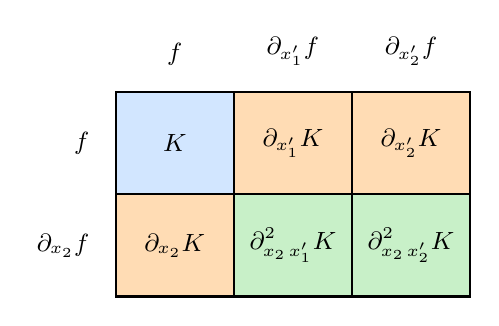
\begin{tikzpicture}
			\def\bw{1.5}
			\def\bh{1.3}

			% Extended Sigma_12^PGEGP: 2x3
			% Top row (f training)
			\fill[ffblock] (0,     \bh) rectangle (\bw,   2*\bh);
			\fill[fdblock] (\bw,   \bh) rectangle (2*\bw, 2*\bh);
			\fill[fdblock] (2*\bw, \bh) rectangle (3*\bw, 2*\bh);
			% Bottom row (dx2 training)
			\fill[fdblock] (0,     0)   rectangle (\bw,   \bh);
			\fill[ddblock] (\bw,   0)   rectangle (2*\bw, \bh);
			\fill[ddblock] (2*\bw, 0)   rectangle (3*\bw, \bh);

			\draw[black, thick] (0,0) rectangle (3*\bw, 2*\bh);
			\draw[black, thick] (\bw, 0) -- (\bw, 2*\bh);
			\draw[black, thick] (2*\bw, 0) -- (2*\bw, 2*\bh);
			\draw[black, thick] (0, \bh) -- (3*\bw, \bh);

			\node[font=\small] at (0.5*\bw, 1.5*\bh) {$K$};
			\node[font=\small] at (1.5*\bw, 1.5*\bh) {$\partial_{x_1'} K$};
			\node[font=\small] at (2.5*\bw, 1.5*\bh) {$\partial_{x_2'} K$};
			\node[font=\small] at (0.5*\bw, 0.5*\bh) {$\partial_{x_2} K$};
			\node[font=\small] at (1.5*\bw, 0.5*\bh) {$\partial^2_{x_2\,x_1'} K$};
			\node[font=\small] at (2.5*\bw, 0.5*\bh) {$\partial^2_{x_2\,x_2'} K$};

			\node[left=6pt, font=\small] at (0, 1.5*\bh) {$f$};
			\node[left=6pt, font=\small] at (0, 0.5*\bh) {$\partial_{x_2} f$};

			\node[above=6pt, font=\small] at (0.5*\bw, 2*\bh) {$f$};
			\node[above=6pt, font=\small] at (1.5*\bw, 2*\bh) {$\partial_{x_1'} f$};
			\node[above=6pt, font=\small] at (2.5*\bw, 2*\bh) {$\partial_{x_2'} f$};
		\end{tikzpicture}
		\caption{Extended $\boldsymbol{\Sigma}^{\text{PGEGP}}_{12}$}
		\label{fig:pgegp_s12_deriv}
	\end{subfigure}
	\hfill
	\begin{subfigure}[t]{0.48\textwidth}
		\centering
		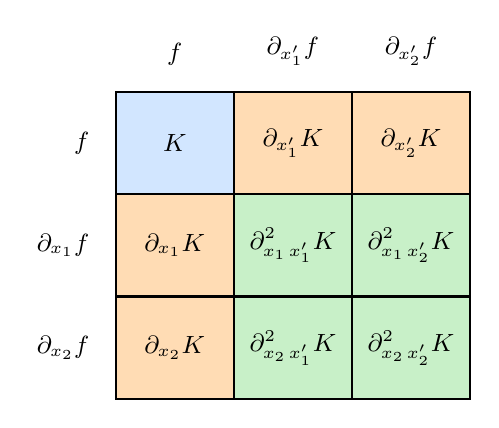
\begin{tikzpicture}
			\def\bw{1.5}
			\def\bh{1.3}

			% Extended Sigma_22^PGEGP: 3x3
			% Top row (f test)
			\fill[ffblock] (0,     2*\bh) rectangle (\bw,   3*\bh);
			\fill[fdblock] (\bw,   2*\bh) rectangle (2*\bw, 3*\bh);
			\fill[fdblock] (2*\bw, 2*\bh) rectangle (3*\bw, 3*\bh);
			% Middle row (dx1 test)
			\fill[fdblock] (0,     \bh)   rectangle (\bw,   2*\bh);
			\fill[ddblock] (\bw,   \bh)   rectangle (2*\bw, 2*\bh);
			\fill[ddblock] (2*\bw, \bh)   rectangle (3*\bw, 2*\bh);
			% Bottom row (dx2 test)
			\fill[fdblock] (0,     0)     rectangle (\bw,   \bh);
			\fill[ddblock] (\bw,   0)     rectangle (2*\bw, \bh);
			\fill[ddblock] (2*\bw, 0)     rectangle (3*\bw, \bh);

			\draw[black, thick] (0,0) rectangle (3*\bw, 3*\bh);
			\draw[black, thick] (\bw, 0) -- (\bw, 3*\bh);
			\draw[black, thick] (2*\bw, 0) -- (2*\bw, 3*\bh);
			\draw[black, thick] (0, \bh) -- (3*\bw, \bh);
			\draw[black, thick] (0, 2*\bh) -- (3*\bw, 2*\bh);

			\node[font=\small] at (0.5*\bw, 2.5*\bh) {$K$};
			\node[font=\small] at (1.5*\bw, 2.5*\bh) {$\partial_{x_1'} K$};
			\node[font=\small] at (2.5*\bw, 2.5*\bh) {$\partial_{x_2'} K$};
			\node[font=\small] at (0.5*\bw, 1.5*\bh) {$\partial_{x_1} K$};
			\node[font=\small] at (1.5*\bw, 1.5*\bh) {$\partial^2_{x_1\,x_1'} K$};
			\node[font=\small] at (2.5*\bw, 1.5*\bh) {$\partial^2_{x_1\,x_2'} K$};
			\node[font=\small] at (0.5*\bw, 0.5*\bh) {$\partial_{x_2} K$};
			\node[font=\small] at (1.5*\bw, 0.5*\bh) {$\partial^2_{x_2\,x_1'} K$};
			\node[font=\small] at (2.5*\bw, 0.5*\bh) {$\partial^2_{x_2\,x_2'} K$};

			\node[left=6pt, font=\small] at (0, 2.5*\bh) {$f$};
			\node[left=6pt, font=\small] at (0, 1.5*\bh) {$\partial_{x_1} f$};
			\node[left=6pt, font=\small] at (0, 0.5*\bh) {$\partial_{x_2} f$};

			\node[above=6pt, font=\small] at (0.5*\bw, 3*\bh) {$f$};
			\node[above=6pt, font=\small] at (1.5*\bw, 3*\bh) {$\partial_{x_1'} f$};
			\node[above=6pt, font=\small] at (2.5*\bw, 3*\bh) {$\partial_{x_2'} f$};

		\end{tikzpicture}
		\caption{Extended $\boldsymbol{\Sigma}^{\text{PGEGP}}_{22}$}
		\label{fig:pgegp_s22_deriv}
	\end{subfigure}
	\caption{Extended training-test and test-test covariance blocks for a PGEGP with $d=2$ and $\mathbf{X}_A = \{x_2\}$, when predicting function values and all partial derivatives at test locations. The training side (rows of $\boldsymbol{\Sigma}_{12}$) retains only $f$ and $\partial_{x_2} f$, while the test side (columns) is extended to include $\partial_{x_1} f$. The resulting $\boldsymbol{\Sigma}_{12}$ is $2n \times 3n_*$ and $\boldsymbol{\Sigma}_{22}$ is $3n_* \times 3n_*$.}
	\label{fig:pgegp_deriv_prediction}
\end{figure}

The key advantage of PGEGP is the reduction in covariance matrix size from $n(d+1) \times n(d+1)$ to $n(m+1) \times n(m+1)$, where $m \ll d$, resulting in substantial computational savings while retaining the most informative derivative information. Studies have demonstrated that PGEGP can reduce modeling time by 30-60\% compared to full GEGP while maintaining or even improving accuracy in some cases~\cite{CHEN201915}. 


\subsection{Directional Derivative-Enhanced Gaussian Processes}
\label{subsec:ddgp}
First-order directional derivatives offer an alternative approach to incorporating derivative information in Gaussian processes~\cite{Yao2024-hp, Padidar2021-fr}. Rather than using all $d$ partial derivatives at each training point as in GEGP, directional derivative GPs (DDGP) use only $q \ll d$ derivatives along user-selected directions. This reduces computational cost while still capturing important local geometric information. A key feature of this approach is that the directions can be chosen uniquely for each training point, allowing for a more flexible and adaptive model.

\subsubsection{Formulation}
\label{subsubsec:ddgp_formulation}

For a training point $\mathbf{x}_i$, let $\mathbf{v}_{i,j} \in \mathbb{R}^d$ denote the $j$-th direction vector (with $\|\mathbf{v}_{i,j}\| = 1$), for $j = 1, \ldots, q$. The directional derivative of $f$ at $\mathbf{x}_i$ along direction $\mathbf{v}_{i,j}$ is:
\begin{equation}
	\partial_{\mathbf{v}_{i,j}} f(\mathbf{x}_i) = \nabla f(\mathbf{x}_i)^T \mathbf{v}_{i,j} = \sum_{k=1}^{d} \partial_{x_k} f(\mathbf{x}_i) \, v_{i,j,k}.
\end{equation}

The training data is augmented with $q$ directional derivatives at each of the $n$ points. Let $\mathbf{V} = \{\mathbf{v}_{i,j} \mid i = 1,\ldots,n, \, j = 1,\ldots,q\}$ denote the collection of all training direction vectors. For predictions at $n_*$ test locations $\mathbf{X}_*$ with $q_*$ direction vectors per point, collected in $\mathbf{V}_* = \{\mathbf{v}_{*i,j} \mid i = 1,\ldots,n_*, \, j = 1,\ldots,q_*\}$, the augmented training and test vectors are:
\begin{equation}
	\label{eqn:ddgp_bg_aug_vector}
	\mathbf{y}^{DD} = \begin{bmatrix}
		f(\mathbf{x}_1) \\
		\vdots \\
		f(\mathbf{x}_n) \\
		\partial_{\mathbf{v}_{1,1}} f(\mathbf{x}_1) \\
		\vdots \\
		\partial_{\mathbf{v}_{1,q}} f(\mathbf{x}_1) \\
		\vdots \\
		\partial_{\mathbf{v}_{n,q}} f(\mathbf{x}_n)
	\end{bmatrix} \in \mathbb{R}^{n(1+q)}, \quad
	\mathbf{y}^{DD}_* = \begin{bmatrix}
		f(\mathbf{x}_{*1}) \\
		\vdots \\
		f(\mathbf{x}_{*n_*}) \\
		\partial_{\mathbf{v}_{*1,1}} f(\mathbf{x}_{*1}) \\
		\vdots \\
		\partial_{\mathbf{v}_{*1,q_*}} f(\mathbf{x}_{*1}) \\
		\vdots \\
		\partial_{\mathbf{v}_{*n_*,q_*}} f(\mathbf{x}_{*n_*})
	\end{bmatrix} \in \mathbb{R}^{n_*(1+q_*)}.
\end{equation}

The joint distribution over the augmented training and test vectors is multivariate Gaussian:
\begin{equation}
	\label{eqn:ddgp_bg_joint}
	\begin{pmatrix}
		\mathbf{y}^{DD} \\
		\mathbf{y}^{DD}_*
	\end{pmatrix}
	\sim \mathcal{N}\left(
	\mathbf{0},
	\begin{pmatrix}
		\boldsymbol{\Sigma}_{11}^{DD} & \boldsymbol{\Sigma}_{12}^{DD} \\
		\boldsymbol{\Sigma}_{21}^{DD} & \boldsymbol{\Sigma}_{22}^{DD}
	\end{pmatrix}
	\right).
\end{equation}

The training covariance block $\boldsymbol{\Sigma}_{11}^{DD}$ is an $n(1+q) \times n(1+q)$ matrix with block structure:
\begin{equation}
	\label{eqn:ddgp_bg_S11}
	\boldsymbol{\Sigma}_{11}^{DD} =
	\begin{pmatrix}
		K & \partial_{\mathbf{V}'} K \\
		\partial_{\mathbf{V}} K & \partial^2_{\mathbf{V}\,\mathbf{V}'} K
	\end{pmatrix}.
\end{equation}
Here $K$ is $n \times n$, the off-diagonal blocks $\partial_{\mathbf{V}} K$ are $nq \times n$, and the lower-right block $\partial^2_{\mathbf{V}\,\mathbf{V}'} K$ is $nq \times nq$.

To make this concrete, consider $d = 2$ with $n = 2$ training points and $q = 1$ direction per point. Since $q = 1$,  $\mathbf{v}_i$ is written for the single direction at $\mathbf{x}_i$. The augmented training vector has $n(1+q) = 4$ entries:
\begin{equation}
	\label{eqn:ddgp_aug_vector_2d}
	\mathbf{y}^{DD} = \begin{bmatrix} f(\mathbf{x}_1) \\ f(\mathbf{x}_2) \\ \partial_{\mathbf{v}_1} f(\mathbf{x}_1) \\ \partial_{\mathbf{v}_2} f(\mathbf{x}_2) \end{bmatrix} \in \mathbb{R}^{4},
\end{equation}
and the training covariance block is the following $4 \times 4$ matrix, where $K_{ij} = K(\mathbf{x}_i, \mathbf{x}_j)$:
\begin{equation}
	\label{eqn:ddgp_S11_2d}
	\resizebox{0.50\textwidth}{!}{$\displaystyle
	\boldsymbol{\Sigma}_{11}^{DD} =
	\begin{pmatrix}
		K_{11} & K_{12} & \partial_{\mathbf{v}_1'} K_{11} & \partial_{\mathbf{v}_2'} K_{12} \\[8pt]
		K_{21} & K_{22} & \partial_{\mathbf{v}_1'} K_{21} & \partial_{\mathbf{v}_2'} K_{22} \\[8pt]
		\partial_{\mathbf{v}_1} K_{11} & \partial_{\mathbf{v}_1} K_{12} & \partial^2_{\mathbf{v}_1\,\mathbf{v}_1'} K_{11} & \partial^2_{\mathbf{v}_1\,\mathbf{v}_2'} K_{12} \\[8pt]
		\partial_{\mathbf{v}_2} K_{21} & \partial_{\mathbf{v}_2} K_{22} & \partial^2_{\mathbf{v}_2\,\mathbf{v}_1'} K_{21} & \partial^2_{\mathbf{v}_2\,\mathbf{v}_2'} K_{22}
	\end{pmatrix}.
	$}
\end{equation}
Each $2 \times 2$ block corresponds to one of the blocks in \eqref{eqn:ddgp_bg_S11}, expanded element-wise across training points. Note that each training point has its own direction vector $\mathbf{v}_i$, so the derivative entries are not uniform across rows and columns---this is a key distinction from GEGP, where all points share the same coordinate directions. The block structure is illustrated in Figure~\ref{fig:ddgp_cov_structure_2d}.
\begin{figure}[htbp]
	\centering
	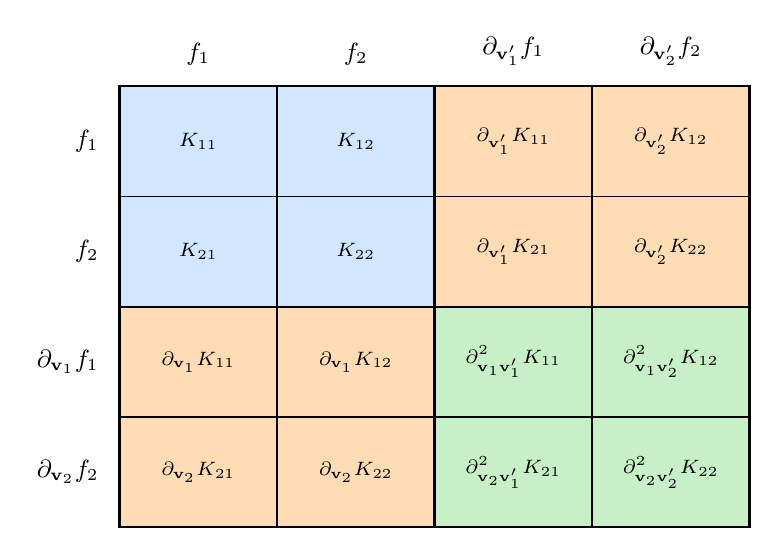
\begin{tikzpicture}
		\def\bw{2.0}
		\def\bh{1.4}

		% --- Colored blocks ---
		\fill[ffblock] (0, 2*\bh) rectangle (2*\bw, 4*\bh);
		\fill[fdblock] (2*\bw, 2*\bh) rectangle (4*\bw, 4*\bh);
		\fill[fdblock] (0, 0) rectangle (2*\bw, 2*\bh);
		\fill[ddblock] (2*\bw, 0) rectangle (4*\bw, 2*\bh);

		% --- Cell grid lines (thin) ---
		\draw[black, thin] (1*\bw, 0) -- (1*\bw, 4*\bh);
		\draw[black, thin] (3*\bw, 0) -- (3*\bw, 4*\bh);
		\draw[black, thin] (0, 1*\bh) -- (4*\bw, 1*\bh);
		\draw[black, thin] (0, 3*\bh) -- (4*\bw, 3*\bh);

		% --- Block boundaries (thick) ---
		\draw[black, thick] (0,0) rectangle (4*\bw, 4*\bh);
		\draw[black, thick] (2*\bw, 0) -- (2*\bw, 4*\bh);
		\draw[black, thick] (0, 2*\bh) -- (4*\bw, 2*\bh);

		% --- Cell labels: ff block (top-left 2x2) ---
		\node[font=\scriptsize] at (0.5*\bw, 3.5*\bh) {$K_{11}$};
		\node[font=\scriptsize] at (1.5*\bw, 3.5*\bh) {$K_{12}$};
		\node[font=\scriptsize] at (0.5*\bw, 2.5*\bh) {$K_{21}$};
		\node[font=\scriptsize] at (1.5*\bw, 2.5*\bh) {$K_{22}$};

		% --- Cell labels: fv block (top-right 2x2) ---
		\node[font=\scriptsize] at (2.5*\bw, 3.5*\bh) {$\partial_{\mathbf{v}_1'} K_{11}$};
		\node[font=\scriptsize] at (3.5*\bw, 3.5*\bh) {$\partial_{\mathbf{v}_2'} K_{12}$};
		\node[font=\scriptsize] at (2.5*\bw, 2.5*\bh) {$\partial_{\mathbf{v}_1'} K_{21}$};
		\node[font=\scriptsize] at (3.5*\bw, 2.5*\bh) {$\partial_{\mathbf{v}_2'} K_{22}$};

		% --- Cell labels: vf block (bottom-left 2x2) ---
		\node[font=\scriptsize] at (0.5*\bw, 1.5*\bh) {$\partial_{\mathbf{v}_1} K_{11}$};
		\node[font=\scriptsize] at (1.5*\bw, 1.5*\bh) {$\partial_{\mathbf{v}_1} K_{12}$};
		\node[font=\scriptsize] at (0.5*\bw, 0.5*\bh) {$\partial_{\mathbf{v}_2} K_{21}$};
		\node[font=\scriptsize] at (1.5*\bw, 0.5*\bh) {$\partial_{\mathbf{v}_2} K_{22}$};

		% --- Cell labels: vv block (bottom-right 2x2) ---
		\node[font=\scriptsize] at (2.5*\bw, 1.5*\bh) {$\partial^2_{\mathbf{v}_1 \mathbf{v}_1'} K_{11}$};
		\node[font=\scriptsize] at (3.5*\bw, 1.5*\bh) {$\partial^2_{\mathbf{v}_1 \mathbf{v}_2'} K_{12}$};
		\node[font=\scriptsize] at (2.5*\bw, 0.5*\bh) {$\partial^2_{\mathbf{v}_2 \mathbf{v}_1'} K_{21}$};
		\node[font=\scriptsize] at (3.5*\bw, 0.5*\bh) {$\partial^2_{\mathbf{v}_2 \mathbf{v}_2'} K_{22}$};

		% --- Row headers ---
		\node[left=4pt, font=\small] at (0, 3.5*\bh) {$f_1$};
		\node[left=4pt, font=\small] at (0, 2.5*\bh) {$f_2$};
		\node[left=4pt, font=\small] at (0, 1.5*\bh) {$\partial_{\mathbf{v}_1} f_1$};
		\node[left=4pt, font=\small] at (0, 0.5*\bh) {$\partial_{\mathbf{v}_2} f_2$};

		% --- Column headers ---
		\node[above=4pt, font=\small] at (0.5*\bw, 4*\bh) {$f_1$};
		\node[above=4pt, font=\small] at (1.5*\bw, 4*\bh) {$f_2$};
		\node[above=4pt, font=\small] at (2.5*\bw, 4*\bh) {$\partial_{\mathbf{v}_1'} f_1$};
		\node[above=4pt, font=\small] at (3.5*\bw, 4*\bh) {$\partial_{\mathbf{v}_2'} f_2$};
	\end{tikzpicture}

	\vspace{8pt}
	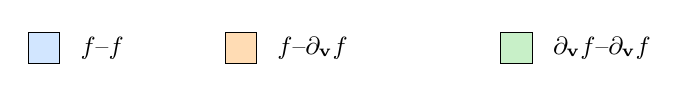
\begin{tikzpicture}
		\fill[ffblock] (0,0) rectangle (0.4, 0.4);
		\draw[black] (0,0) rectangle (0.4, 0.4);
		\node[right=4pt, font=\small] at (0.4, 0.2) {$f$--$f$};

		\fill[fdblock] (2.5,0) rectangle (2.9, 0.4);
		\draw[black] (2.5,0) rectangle (2.9, 0.4);
		\node[right=4pt, font=\small] at (2.9, 0.2) {$f$--$\partial_{\mathbf{v}} f$};

		\fill[ddblock] (6.0,0) rectangle (6.4, 0.4);
		\draw[black] (6.0,0) rectangle (6.4, 0.4);
		\node[right=4pt, font=\small] at (6.4, 0.2) {$\partial_{\mathbf{v}} f$--$\partial_{\mathbf{v}} f$};
	\end{tikzpicture}

	\caption{Element-wise block structure of $\boldsymbol{\Sigma}_{11}^{DD}$ for $d=2$, $n=2$, $q=1$, where $f_i = f(\mathbf{x}_i)$ and $K_{ij} = K(\mathbf{x}_i, \mathbf{x}_j)$. Thick lines delineate the $2 \times 2$ blocks from the general form~\eqref{eqn:ddgp_bg_S11}; thin lines separate individual matrix entries. Each training point has its own direction vector $\mathbf{v}_i$, so derivative entries vary across rows and columns.}
	\label{fig:ddgp_cov_structure_2d}
\end{figure}

The training-test covariance block is:
\begin{equation}
	\label{eqn:ddgp_bg_S12}
	\boldsymbol{\Sigma}_{12}^{DD} =
	\begin{pmatrix}
		K & \partial_{\mathbf{V}_*'} K \\
		\partial_{\mathbf{V}} K & \partial^2_{\mathbf{V}\,\mathbf{V}_*'} K
	\end{pmatrix},
\end{equation}
with $\boldsymbol{\Sigma}_{21}^{DD} = (\boldsymbol{\Sigma}_{12}^{DD})^T$.

The posterior predictive distribution follows the standard GP conditioning formula:
\begin{equation}
	\label{eqn:ddgp_bg_posterior}
	\begin{split}
		\boldsymbol{\mu}^{DD}_{*} &= \boldsymbol{\Sigma}_{21}^{DD} (\boldsymbol{\Sigma}_{11}^{DD})^{-1} \mathbf{y}^{DD}, \\
		\boldsymbol{\Sigma}^{DD}_{*} &=  \boldsymbol{\Sigma}_{22}^{DD} - \boldsymbol{\Sigma}_{21}^{DD} (\boldsymbol{\Sigma}_{11}^{DD})^{-1} \boldsymbol{\Sigma}_{12}^{DD}.
	\end{split}
\end{equation}

Similar to other derivative-enhanced GPs, the kernel hyperparameters $\boldsymbol{\psi}$ are determined by maximizing the log marginal likelihood:
\begin{equation}
	\label{eqn:ddgp_bg_mll}
	\log p(\mathbf{y}^{DD}|\mathbf{X}, \mathbf{V}, \boldsymbol{\psi}) = -\frac{1}{2} (\mathbf{y}^{DD})^\top (\boldsymbol{\Sigma}_{11}^{DD})^{-1} \mathbf{y}^{DD} - \frac{1}{2}\log|\boldsymbol{\Sigma}_{11}^{DD}| - \frac{n(1+q)}{2}\log 2\pi.
\end{equation}

The primary advantage of DDGP is its favorable computational scaling. The matrix to be inverted has dimension $M = n(1+q)$, resulting in $\mathcal{O}((n(1+q))^3)$ complexity. Since $q$ is typically chosen as a small constant ($q \ll d$), this is substantially lower than the $\mathcal{O}((n(d+1))^3)$ cost of full GEGP, making DDGP practical for high-dimensional problems where computing all partial derivatives would be prohibitive. The trade-off is that DDGP captures less geometric information than GEGP, but with careful selection of directions (e.g., along principal curvature directions or gradient directions), it can still provide significant accuracy improvements over standard GP models.

\subsubsection{Selective Derivative Predictions at Test Locations}
\label{subsubsec:ddgp_selective_pred}
As in previous sections, when only function values are required at the test locations, the training-test covariance block simplifies by retaining only the columns corresponding to test function values:
\begin{equation}
	\boldsymbol{\Sigma}_{12}^{DD} \;\longrightarrow\;
	\begin{pmatrix}
		K \\
		\partial_{\mathbf{V}} K
	\end{pmatrix}, \quad \text{and} \quad
	\boldsymbol{\Sigma}_{22}^{DD} \;\longrightarrow\; K.
\end{equation}
The block structure of both the full and reduced forms is illustrated in Figure~\ref{fig:ddgp_s12_reduction}.
\begin{figure}[htbp]
	\centering
	\begin{subfigure}[t]{0.45\textwidth}
		\centering
		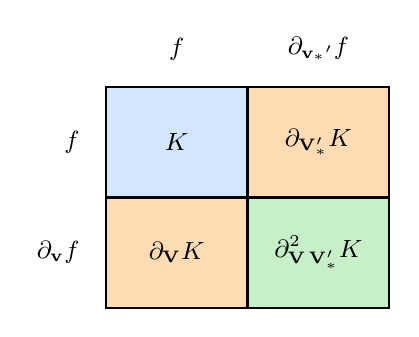
\begin{tikzpicture}
			\def\bw{1.8}
			\def\bh{1.4}
			
			% Full Sigma_12^DD: 2x2
			\fill[ffblock] (0,     \bh) rectangle (\bw,   2*\bh);
			\fill[fdblock] (\bw,   \bh) rectangle (2*\bw, 2*\bh);
			\fill[fdblock] (0,     0)   rectangle (\bw,   \bh);
			\fill[ddblock] (\bw,   0)   rectangle (2*\bw, \bh);
			
			\draw[black, thick] (0,0) rectangle (2*\bw, 2*\bh);
			\draw[black, thick] (\bw, 0) -- (\bw, 2*\bh);
			\draw[black, thick] (0, \bh) -- (2*\bw, \bh);
			
			\node[font=\small] at (0.5*\bw, 1.5*\bh) {$K$};
			\node[font=\small] at (1.5*\bw, 1.5*\bh) {$\partial_{\mathbf{V}_*'} K$};
			\node[font=\small] at (0.5*\bw, 0.5*\bh) {$\partial_{\mathbf{V}} K$};
			\node[font=\small] at (1.5*\bw, 0.5*\bh) {$\partial^2_{\mathbf{V}\,\mathbf{V}_*'} K$};
			
			\node[left=6pt, font=\small] at (0, 1.5*\bh) {$f$};
			\node[left=6pt, font=\small] at (0, 0.5*\bh) {$\partial_{\mathbf{v}} f$};
			
			\node[above=6pt, font=\small] at (0.5*\bw, 2*\bh) {$f$};
			\node[above=6pt, font=\small] at (1.5*\bw, 2*\bh) {$\partial_{\mathbf{v_*}'} f$};
			
		\end{tikzpicture}
		\caption{Full $\boldsymbol{\Sigma}^{DD}_{12}$}
		\label{fig:ddgp_s12_full}
	\end{subfigure}
	\hfill
	\begin{subfigure}[t]{0.45\textwidth}
		\centering
		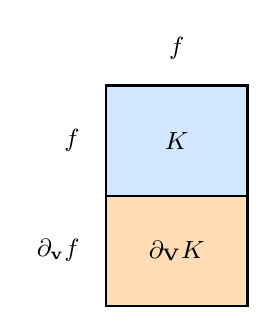
\begin{tikzpicture}
			\def\bw{1.8}
			\def\bh{1.4}
			
			% Reduced Sigma_12^DD: 2x1
			\fill[ffblock] (0, \bh) rectangle (\bw, 2*\bh);
			\fill[fdblock] (0, 0)   rectangle (\bw, \bh);
			
			\draw[black, thick] (0,0) rectangle (\bw, 2*\bh);
			\draw[black, thick] (0, \bh) -- (\bw, \bh);
			
			\node[font=\small] at (0.5*\bw, 1.5*\bh) {$K$};
			\node[font=\small] at (0.5*\bw, 0.5*\bh) {$\partial_{\mathbf{V}} K$};
			
			\node[left=6pt, font=\small] at (0, 1.5*\bh) {$f$};
			\node[left=6pt, font=\small] at (0, 0.5*\bh) {$\partial_{\mathbf{v}} f$};
			
			\node[above=6pt, font=\small] at (0.5*\bw, 2*\bh) {$f$};
			
		\end{tikzpicture}
		\caption{Reduced $\boldsymbol{\Sigma}^{DD}_{12}$}
		\label{fig:ddgp_s12_reduced}
	\end{subfigure}
	\caption{Full (left) and reduced (right) training-test covariance block $\boldsymbol{\Sigma}^{DD}_{12}$ for a DDGP with $q$ directional derivatives per training point, when only function values are predicted at test locations. The reduced form retains only the first column of blocks, reducing from an $n(1+q) \times n_*(1+q_*)$ matrix to an $n(1+q) \times n_*$ matrix.}
	\label{fig:ddgp_s12_reduction}
\end{figure}

Although only directional derivatives along the training directions in $\mathbf{V}$ are used during training, predictions at test locations can be made along any set of directions by choosing the test direction vectors $\mathbf{V}_*$ freely when constructing $\boldsymbol{\Sigma}_{12}^{DD}$ and $\boldsymbol{\Sigma}_{22}^{DD}$. In particular, the number of test directions $q_*$ need not equal the number of training directions $q$, and the test directions themselves are entirely independent of the training directions $\mathbf{V}$, while the training covariance $\boldsymbol{\Sigma}_{11}^{DD}$ remains unchanged.


	Continuing the $d=2$, $q=1$ example, suppose we wish to predict directional derivatives along $q_* = 2$ directions at each test point, in addition to function values. Let $\mathbf{V}_{*,1} = \{\mathbf{v}_{*i,1}\}_{i=1}^{n_*}$ and $\mathbf{V}_{*,2} = \{\mathbf{v}_{*i,2}\}_{i=1}^{n_*}$ denote the two sets of test direction vectors. The training-test covariance block is
	\begin{equation}
		\boldsymbol{\Sigma}_{12}^{DD} =
		\begin{pmatrix}
			K & \partial_{\mathbf{V}_{*,1}'} K & \partial_{\mathbf{V}_{*,2}'} K \\[8pt]
			\partial_{\mathbf{V}} K & \partial^2_{\mathbf{V}\,\mathbf{V}_{*,1}'} K & \partial^2_{\mathbf{V}\,\mathbf{V}_{*,2}'} K
		\end{pmatrix},
	\end{equation}
	and the test covariance block becomes the full $3n_* \times 3n_*$ matrix
	\begin{equation}
		\boldsymbol{\Sigma}_{22}^{DD} =
		\begin{pmatrix}
			K & \partial_{\mathbf{V}_{*,1}'} K & \partial_{\mathbf{V}_{*,2}'} K \\[8pt]
			\partial_{\mathbf{V}_{*,1}} K & \partial^2_{\mathbf{V}_{*,1}\,\mathbf{V}_{*,1}'} K & \partial^2_{\mathbf{V}_{*,1}\,\mathbf{V}_{*,2}'} K \\[8pt]
			\partial_{\mathbf{V}_{*,2}} K & \partial^2_{\mathbf{V}_{*,2}\,\mathbf{V}_{*,1}'} K & \partial^2_{\mathbf{V}_{*,2}\,\mathbf{V}_{*,2}'} K
		\end{pmatrix}.
	\end{equation}
	Note that $\boldsymbol{\Sigma}_{11}^{DD}$ remains $n(1+q) \times n(1+q)$ — only the test-side blocks are extended. The resulting $\boldsymbol{\Sigma}_{12}$ is $n(1+q) \times n_*(1+q_*)$ and $\boldsymbol{\Sigma}_{22}$ is $n_*(1+q_*) \times n_*(1+q_*)$. The block structure of the extended forms is illustrated in Figure~\ref{fig:ddgp_deriv_prediction}. More generally, predictions for any number of directional derivatives along arbitrary test directions can be obtained by constructing $\boldsymbol{\Sigma}_{12}$ and $\boldsymbol{\Sigma}_{22}$ with the appropriate directional derivative kernel blocks, without modifying the training side.
\begin{figure}[htbp]
	\centering
	\begin{subfigure}[t]{0.48\textwidth}
		\centering
		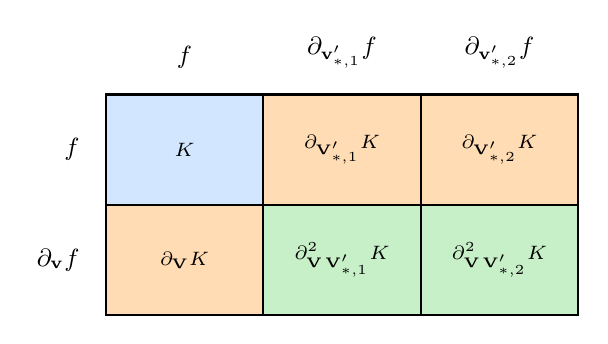
\begin{tikzpicture}
			\def\bw{2.0}
			\def\bh{1.4}

			% Extended Sigma_12^DD: 2x3
			% Top row (f training)
			\fill[ffblock] (0,     \bh) rectangle (\bw,   2*\bh);
			\fill[fdblock] (\bw,   \bh) rectangle (2*\bw, 2*\bh);
			\fill[fdblock] (2*\bw, \bh) rectangle (3*\bw, 2*\bh);
			% Bottom row (dv training)
			\fill[fdblock] (0,     0)   rectangle (\bw,   \bh);
			\fill[ddblock] (\bw,   0)   rectangle (2*\bw, \bh);
			\fill[ddblock] (2*\bw, 0)   rectangle (3*\bw, \bh);

			\draw[black, thick] (0,0) rectangle (3*\bw, 2*\bh);
			\draw[black, thick] (\bw, 0) -- (\bw, 2*\bh);
			\draw[black, thick] (2*\bw, 0) -- (2*\bw, 2*\bh);
			\draw[black, thick] (0, \bh) -- (3*\bw, \bh);

			\node[font=\scriptsize] at (0.5*\bw, 1.5*\bh) {$K$};
			\node[font=\scriptsize] at (1.5*\bw, 1.5*\bh) {$\partial_{\mathbf{V}_{*,1}'} K$};
			\node[font=\scriptsize] at (2.5*\bw, 1.5*\bh) {$\partial_{\mathbf{V}_{*,2}'} K$};
			\node[font=\scriptsize] at (0.5*\bw, 0.5*\bh) {$\partial_{\mathbf{V}} K$};
			\node[font=\scriptsize] at (1.5*\bw, 0.5*\bh) {$\partial^2_{\mathbf{V}\,\mathbf{V}_{*,1}'} K$};
			\node[font=\scriptsize] at (2.5*\bw, 0.5*\bh) {$\partial^2_{\mathbf{V}\,\mathbf{V}_{*,2}'} K$};

			\node[left=6pt, font=\small] at (0, 1.5*\bh) {$f$};
			\node[left=6pt, font=\small] at (0, 0.5*\bh) {$\partial_{\mathbf{v}} f$};

			\node[above=6pt, font=\small] at (0.5*\bw, 2*\bh) {$f$};
			\node[above=6pt, font=\small] at (1.5*\bw, 2*\bh) {$\partial_{\mathbf{v}'_{*,1}} f$};
			\node[above=6pt, font=\small] at (2.5*\bw, 2*\bh) {$\partial_{\mathbf{v}'_{*,2}} f$};

		\end{tikzpicture}
		\caption{Extended $\boldsymbol{\Sigma}^{DD}_{12}$}
		\label{fig:ddgp_s12_deriv}
	\end{subfigure}
	\hfill
	\begin{subfigure}[t]{0.48\textwidth}
		\centering
		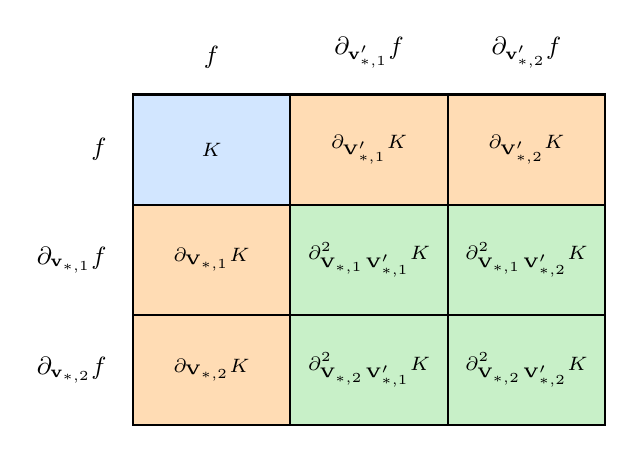
\begin{tikzpicture}
			\def\bw{2.0}
			\def\bh{1.4}

			% Extended Sigma_22^DD: 3x3
			% Top row (f test)
			\fill[ffblock] (0,     2*\bh) rectangle (\bw,   3*\bh);
			\fill[fdblock] (\bw,   2*\bh) rectangle (2*\bw, 3*\bh);
			\fill[fdblock] (2*\bw, 2*\bh) rectangle (3*\bw, 3*\bh);
			% Middle row (dv*1 test)
			\fill[fdblock] (0,     \bh)   rectangle (\bw,   2*\bh);
			\fill[ddblock] (\bw,   \bh)   rectangle (2*\bw, 2*\bh);
			\fill[ddblock] (2*\bw, \bh)   rectangle (3*\bw, 2*\bh);
			% Bottom row (dv*2 test)
			\fill[fdblock] (0,     0)     rectangle (\bw,   \bh);
			\fill[ddblock] (\bw,   0)     rectangle (2*\bw, \bh);
			\fill[ddblock] (2*\bw, 0)     rectangle (3*\bw, \bh);

			\draw[black, thick] (0,0) rectangle (3*\bw, 3*\bh);
			\draw[black, thick] (\bw, 0) -- (\bw, 3*\bh);
			\draw[black, thick] (2*\bw, 0) -- (2*\bw, 3*\bh);
			\draw[black, thick] (0, \bh) -- (3*\bw, \bh);
			\draw[black, thick] (0, 2*\bh) -- (3*\bw, 2*\bh);

			\node[font=\scriptsize] at (0.5*\bw, 2.5*\bh) {$K$};
			\node[font=\scriptsize] at (1.5*\bw, 2.5*\bh) {$\partial_{\mathbf{V}_{*,1}'} K$};
			\node[font=\scriptsize] at (2.5*\bw, 2.5*\bh) {$\partial_{\mathbf{V}_{*,2}'} K$};
			\node[font=\scriptsize] at (0.5*\bw, 1.5*\bh) {$\partial_{\mathbf{V}_{*,1}} K$};
			\node[font=\scriptsize] at (1.5*\bw, 1.5*\bh) {$\partial^2_{\mathbf{V}_{*,1}\,\mathbf{V}_{*,1}'} K$};
			\node[font=\scriptsize] at (2.5*\bw, 1.5*\bh) {$\partial^2_{\mathbf{V}_{*,1}\,\mathbf{V}_{*,2}'} K$};
			\node[font=\scriptsize] at (0.5*\bw, 0.5*\bh) {$\partial_{\mathbf{V}_{*,2}} K$};
			\node[font=\scriptsize] at (1.5*\bw, 0.5*\bh) {$\partial^2_{\mathbf{V}_{*,2}\,\mathbf{V}_{*,1}'} K$};
			\node[font=\scriptsize] at (2.5*\bw, 0.5*\bh) {$\partial^2_{\mathbf{V}_{*,2}\,\mathbf{V}_{*,2}'} K$};

			\node[left=6pt, font=\small] at (0, 2.5*\bh) {$f$};
			\node[left=6pt, font=\small] at (0, 1.5*\bh) {$\partial_{\mathbf{v}_{*,1}} f$};
			\node[left=6pt, font=\small] at (0, 0.5*\bh) {$\partial_{\mathbf{v}_{*,2}} f$};

			\node[above=6pt, font=\small] at (0.5*\bw, 3*\bh) {$f$};
			\node[above=6pt, font=\small] at (1.5*\bw, 3*\bh) {$\partial_{\mathbf{v}'_{*,1}} f$};
			\node[above=6pt, font=\small] at (2.5*\bw, 3*\bh) {$\partial_{\mathbf{v}'_{*,2}} f$};

		\end{tikzpicture}
		\caption{Extended $\boldsymbol{\Sigma}^{DD}_{22}$}
		\label{fig:ddgp_s22_deriv}
	\end{subfigure}
	\caption{Extended training-test and test-test covariance blocks for a DDGP with $q=1$ training direction per point, when predicting function values and $q_*=2$ directional derivatives at test locations. The training side (rows of $\boldsymbol{\Sigma}_{12}$) retains only $f$ and $\partial_{\mathbf{v}} f$, while the test side (columns) is extended to include two independent test direction sets $\mathbf{V}_{*,1}$ and $\mathbf{V}_{*,2}$. The resulting $\boldsymbol{\Sigma}_{12}$ is $2n \times 3n_*$ and $\boldsymbol{\Sigma}_{22}$ is $3n_* \times 3n_*$.}
	\label{fig:ddgp_deriv_prediction}
\end{figure}

\paragraph{Numerical example.}
Using the same test function and training grid, the DDGP replaces the two coordinate-aligned partial derivatives with directional derivatives along $\mathbf{v}_1 = (\cos 45^\circ, \sin 45^\circ)$ and $\mathbf{v}_2 = (\cos 135^\circ, \sin 135^\circ)$. With $q = 2$ directions, the covariance matrix has the same dimension $n(1 + q) = 75$ as the GEGP's $n(1 + d) = 75$ for this two-dimensional problem. Figure~\ref{fig:ddgp_example} shows the function and directional derivative predictions. The DDGP achieves comparable accuracy to the GEGP while using derivative information along non-coordinate directions. In higher-dimensional problems where $d \gg q$, the DDGP offers substantial computational savings since the matrix size depends on $q$ rather than $d$.

\begin{figure}[H]
	\centering
	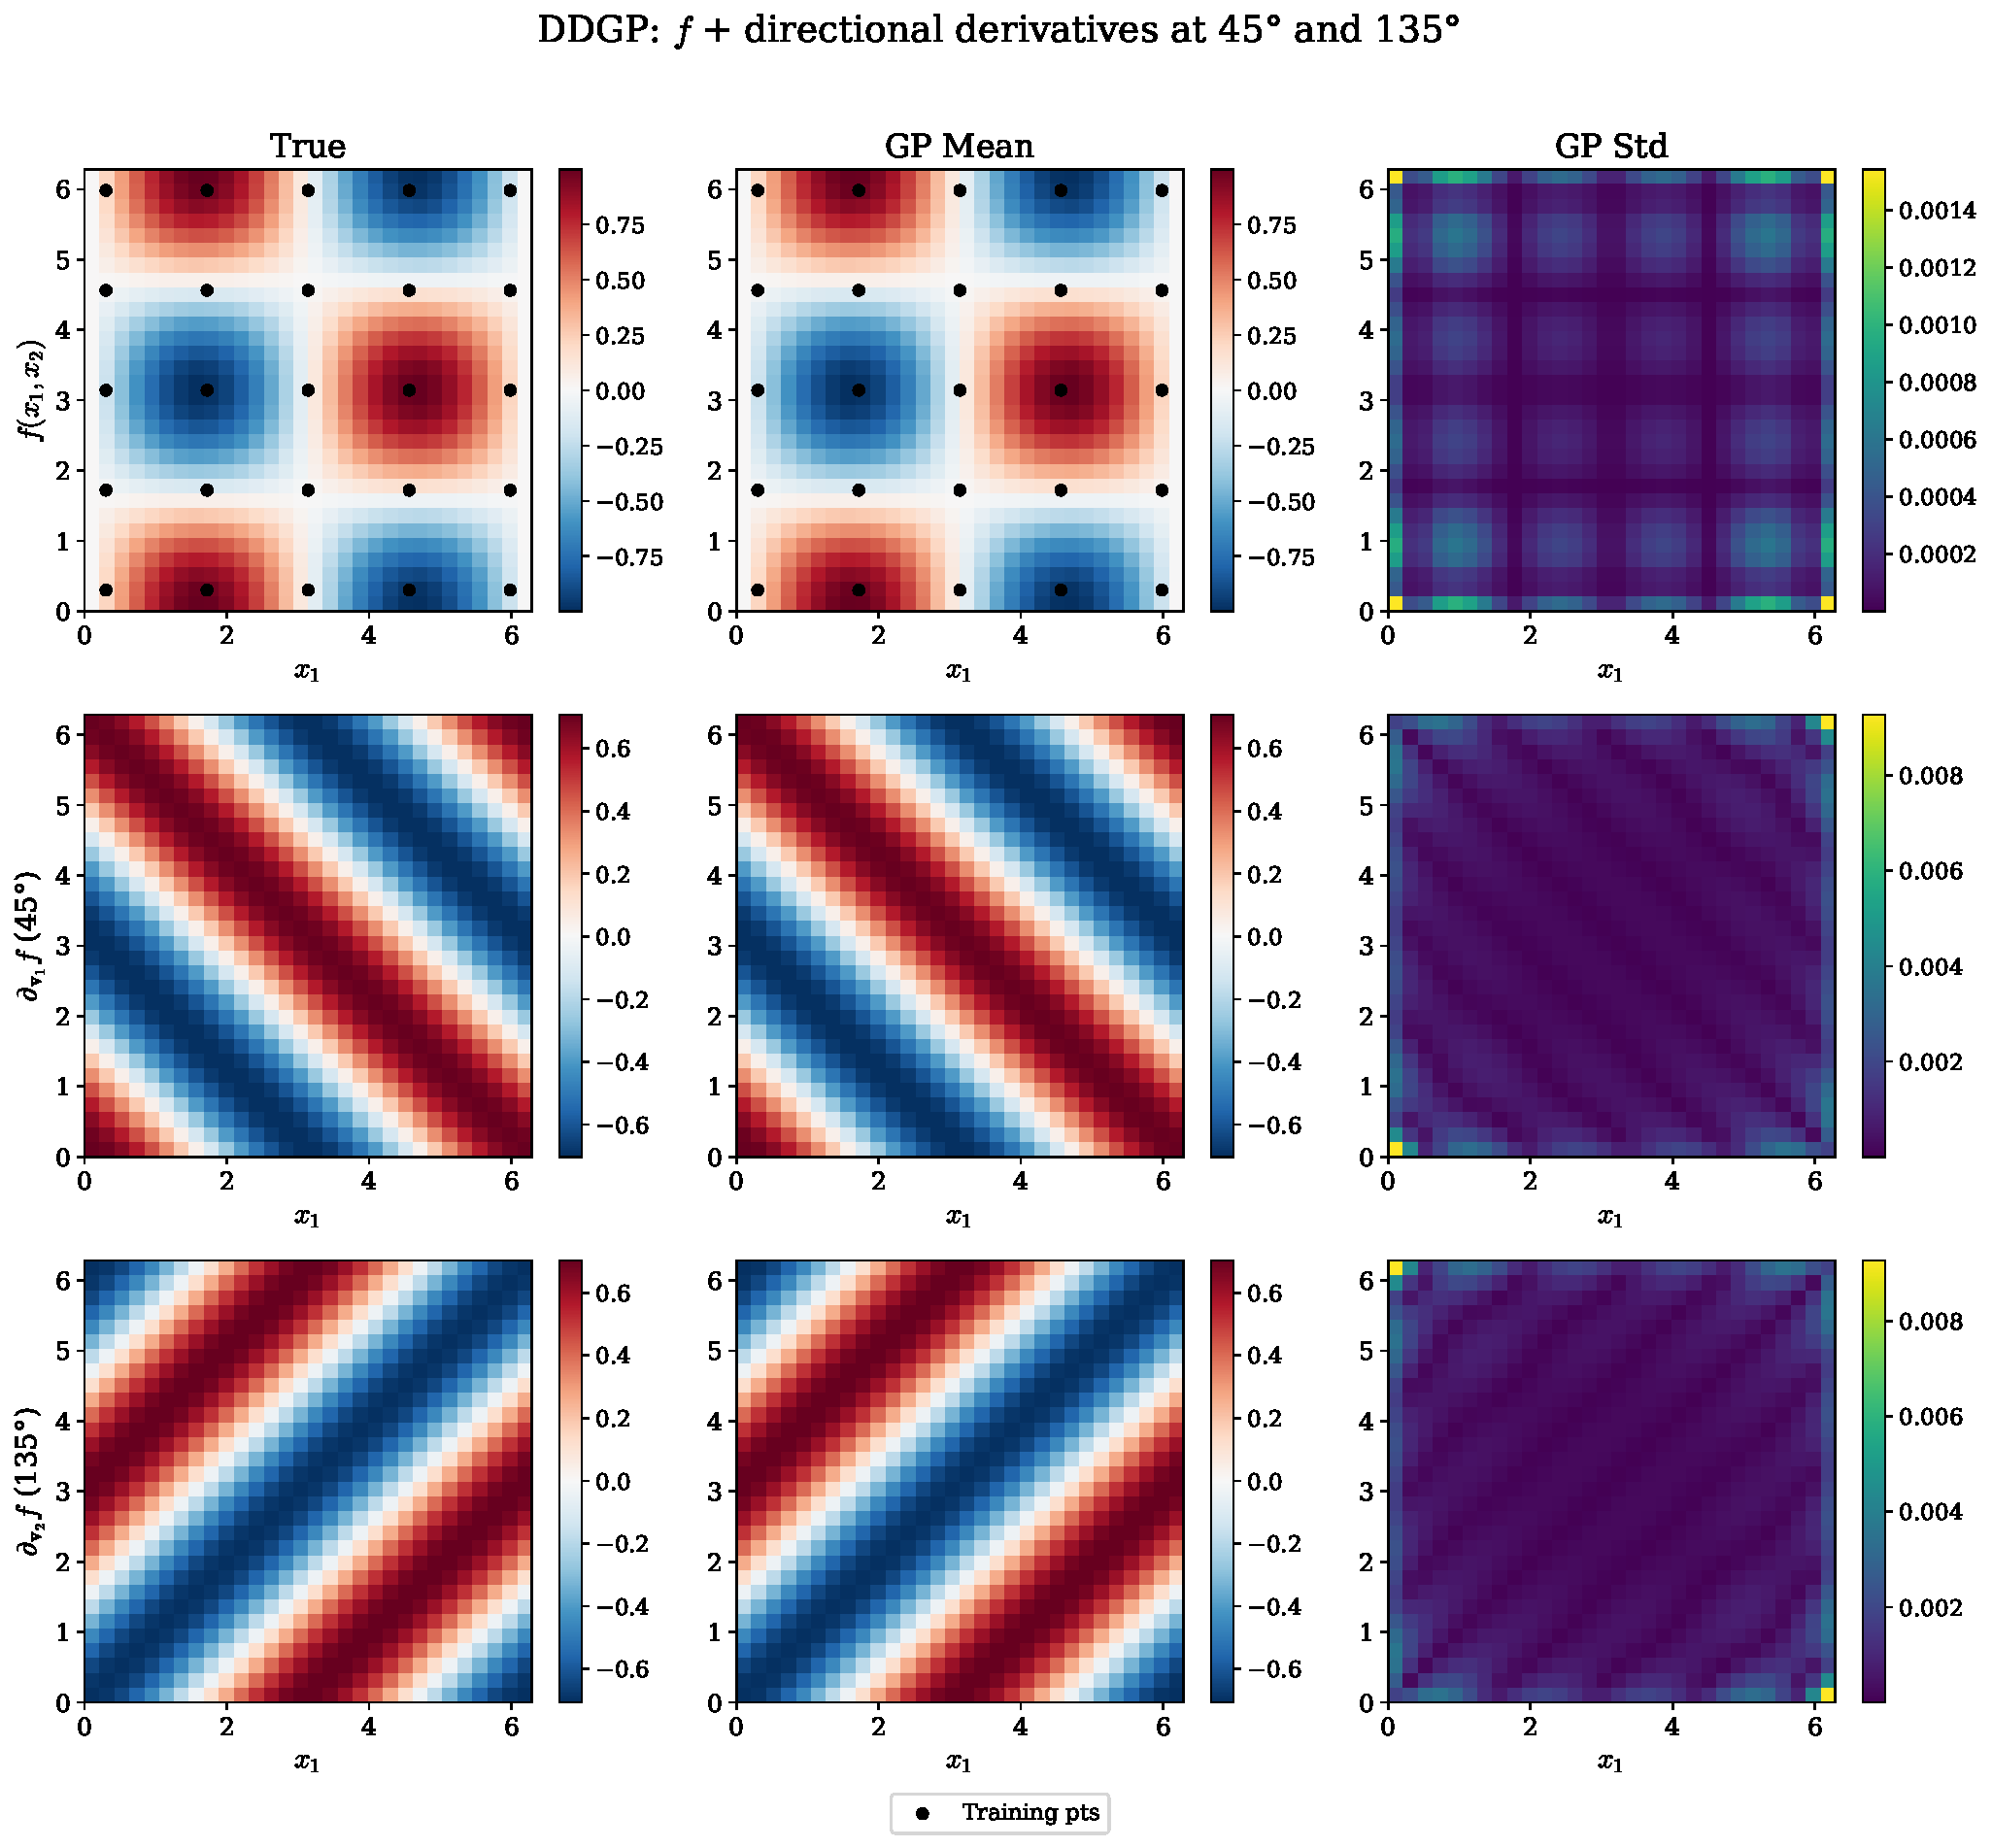
\includegraphics[width=\textwidth]{ddgp_example.pdf}
	\caption{DDGP example on $f(x_1, x_2) = \sin(x_1)\cos(x_2)$ with $n = 25$ training points and $q = 2$ directional derivatives at $45^\circ$ and $135^\circ$. Rows show $f$, $\partial_{\mathbf{v}_1} f$, and $\partial_{\mathbf{v}_2} f$; columns show the true function, GP posterior mean, and posterior standard deviation.}
	\label{fig:ddgp_example}
\end{figure}

%==============================================================================
\subsection{Reduced Gradient-Enhanced Gaussian Processes}
\label{subsec:rdgegp}
%==============================================================================

In the preceding sections, every training point is assumed to have derivative information---either full gradients (GEGP), Hessians (HEGP), a selected subset of partial derivatives (PGEGP), or directional derivatives (DDGP). In practice, however, derivative information may not be available at every training point. Gradient evaluations can be expensive, partially observed, or deliberately skipped at some locations to reduce computational cost~\cite{CHEN2020112861}. The Reduced Gradient-Enhanced GP (RdGEGP) accommodates this setting: all $n$ training points contribute function values, but only a subset of $n_g \leq n$ points contribute gradient observations.

\subsubsection{Formulation}
\label{subsubsec:rdgegp_formulation}

Let $\mathcal{I}_g \subseteq \{1, \ldots, n\}$ with $|\mathcal{I}_g| = n_g$ denote the indices of training points at which gradient information is available, and let $\mathbf{X}_g = \{\mathbf{x}_i \mid i \in \mathcal{I}_g\}$ denote the corresponding locations. The augmented training and test vectors are:
\begin{equation}
	\label{eqn:rdgegp_aug_vectors}
	\mathbf{y}^{R} = \begin{bmatrix} f(\mathbf{X}) \\ \nabla f(\mathbf{X}_g) \end{bmatrix} \in \mathbb{R}^{n + d \cdot n_g}, \quad
	\mathbf{y}^{R}_* = \begin{bmatrix} f(\mathbf{X}_*) \\ \nabla f(\mathbf{X}_*) \end{bmatrix}.
\end{equation}
Note that the training vector $\mathbf{y}^R$ contains function values at all $n$ points but gradient information only at the $n_g$ gradient-observed points in $\mathbf{X}_g$, producing an asymmetric structure. The test vector $\mathbf{y}^R_*$ may include full derivative predictions at all test locations.

The joint distribution over the augmented training and test vectors is multivariate Gaussian:
\begin{equation}
	\label{eqn:rdgegp_joint_dist}
	\begin{pmatrix}
		\mathbf{y}^{R} \\
		\mathbf{y}^{R}_*
	\end{pmatrix}
	\sim \mathcal{N}\left(
	\mathbf{0},
	\begin{pmatrix}
		\boldsymbol{\Sigma}^{R}_{11} & \boldsymbol{\Sigma}^{R}_{12} \\
		\boldsymbol{\Sigma}^{R}_{21} & \boldsymbol{\Sigma}^{R}_{22}
	\end{pmatrix}
	\right).
\end{equation}

The training covariance block $\boldsymbol{\Sigma}^{R}_{11}$ is an $(n + d \cdot n_g) \times (n + d \cdot n_g)$ matrix:
\begin{equation}
	\label{eqn:rdgegp_S11}
	\boldsymbol{\Sigma}^{R}_{11} =
	\begin{pmatrix}
		K & \partial_{\mathbf{X}_g'} K \\
		\partial_{\mathbf{X}_g} K & \partial^2_{\mathbf{X}_g\,\mathbf{X}_g'} K
	\end{pmatrix}.
\end{equation}
Here $K$ is $n \times n$, the off-diagonal block $\partial_{\mathbf{X}_g'} K$ is $n \times d \cdot n_g$, and the lower-right block $\partial^2_{\mathbf{X}_g\,\mathbf{X}_g'} K$ is $d \cdot n_g \times d \cdot n_g$. This asymmetry---$n$ in the function dimension versus $n_g$ in the derivative dimensions---is the defining feature of the RdGEGP covariance structure.

The full training-test covariance block, including derivative predictions at test points, is:
\begin{equation}
	\label{eqn:rdgegp_S12_full}
	\boldsymbol{\Sigma}^{R}_{12} =
	\begin{pmatrix}
		K & \partial_{\mathbf{X}_*'} K \\
		\partial_{\mathbf{X}_g} K & \partial^2_{\mathbf{X}_g\,\mathbf{X}_*'} K
	\end{pmatrix}.
\end{equation}

The posterior predictive distribution follows the standard GP conditioning formula:
\begin{equation}
	\label{eqn:rdgegp_posterior}
	\begin{split}
		\boldsymbol{\mu}^{R}_{*} &= \boldsymbol{\Sigma}^{R}_{21} \left(\boldsymbol{\Sigma}^{R}_{11}\right)^{-1} \mathbf{y}^{R}, \\
		\boldsymbol{\Sigma}^{R}_{*} &= \boldsymbol{\Sigma}^{R}_{22} - \boldsymbol{\Sigma}^{R}_{21} \left(\boldsymbol{\Sigma}^{R}_{11}\right)^{-1} \boldsymbol{\Sigma}^{R}_{12}.
	\end{split}
\end{equation}

Similar to other derivative-enhanced GPs, the kernel hyperparameters $\boldsymbol{\psi}$ are determined by maximizing the log marginal likelihood (MLL) of the augmented observations:
\begin{equation}
	\label{eqn:rdgegp_mll}
	\log p(\mathbf{y}^{R}|\mathbf{X}, \boldsymbol{\psi}) = -\frac{1}{2} \left(\mathbf{y}^{R}\right)^\top \left(\boldsymbol{\Sigma}^{R}_{11}\right)^{-1} \mathbf{y}^{R} - \frac{1}{2}\log|\boldsymbol{\Sigma}^{R}_{11}| - \frac{n + d \cdot n_g}{2}\log 2\pi.
\end{equation}
The matrix to be decomposed has dimension $n + d \cdot n_g$, giving a Cholesky cost of $\mathcal{O}((n + d \cdot n_g)^3)$. When $n_g < n$, this is strictly less than the $\mathcal{O}((n(d+1))^3)$ cost of full GEGP; when $n_g = n$, it recovers the GEGP cost.

To make this concrete, consider a function of two variables ($d = 2$) with $n = 3$ training points, of which only $n_g = 2$ (say, points $\mathbf{x}_1$ and $\mathbf{x}_2$) have gradient observations. The augmented training vector is:
\begin{equation}
	\label{eqn:rdgegp_aug_vectors_2d}
	\mathbf{y}^{R} = \begin{bmatrix} f(\mathbf{x}_1) \\ f(\mathbf{x}_2) \\ f(\mathbf{x}_3) \\ \partial_{x_1} f(\mathbf{x}_1) \\ \partial_{x_1} f(\mathbf{x}_2) \\ \partial_{x_2} f(\mathbf{x}_1) \\ \partial_{x_2} f(\mathbf{x}_2) \end{bmatrix} \in \mathbb{R}^{7}.
\end{equation}
Compared to the full GEGP vector of dimension $3n = 9$, the RdGEGP vector omits the derivative entries for $\mathbf{x}_3$, reducing the dimension to $n + d \cdot n_g = 3 + 2 \cdot 2 = 7$.

Figure~\ref{fig:rdgegp_structure_2d} illustrates the reduction from the full GEGP structure to RdGEGP for this example. The excluded entries---derivative rows and columns corresponding to non-gradient training points---are shown in black; arrows indicate how removing these entries yields the reduced RdGEGP training vector and covariance matrix.
\begin{figure}[H]
	\centering

	% === (a) Training vector reduction ===
	\begin{subfigure}[b]{\textwidth}
		\centering
		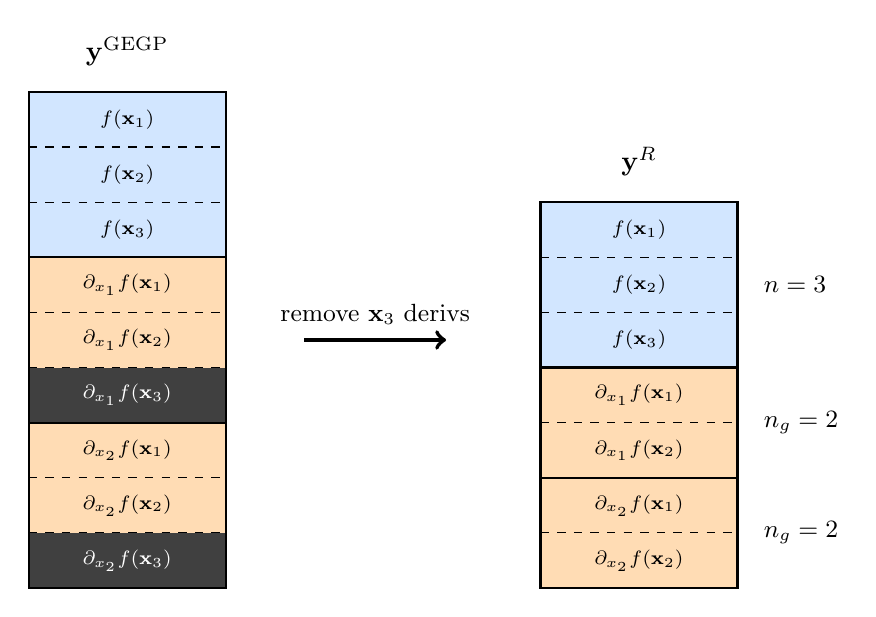
\begin{tikzpicture}
			\def\bw{2.5}
			\def\bh{0.7}

			% --- Left: GEGP vector (3 blocks, each n=3 entries) ---
			% f block (3 entries)
			\fill[ffblock] (0, 6*\bh) rectangle (\bw, 9*\bh);
			% dx1 block (3 entries, entry 3 blacked out)
			\fill[fdblock] (0, 3*\bh) rectangle (\bw, 6*\bh);
			\fill[black!75] (0, 3*\bh) rectangle (\bw, 4*\bh);
			% dx2 block (3 entries, entry 3 blacked out)
			\fill[fdblock] (0, 0) rectangle (\bw, 3*\bh);
			\fill[black!75] (0, 0) rectangle (\bw, 1*\bh);

			% Grid lines
			\draw[black, thick] (0, 0) rectangle (\bw, 9*\bh);
			\draw[black, thick] (0, 6*\bh) -- (\bw, 6*\bh);
			\draw[black, thick] (0, 3*\bh) -- (\bw, 3*\bh);
			% Sub-lines within blocks
			\draw[black, thin, dashed] (0, 7*\bh) -- (\bw, 7*\bh);
			\draw[black, thin, dashed] (0, 8*\bh) -- (\bw, 8*\bh);
			\draw[black, thin, dashed] (0, 4*\bh) -- (\bw, 4*\bh);
			\draw[black, thin, dashed] (0, 5*\bh) -- (\bw, 5*\bh);
			\draw[black, thin, dashed] (0, 1*\bh) -- (\bw, 1*\bh);
			\draw[black, thin, dashed] (0, 2*\bh) -- (\bw, 2*\bh);

			% Labels
			\node[font=\scriptsize] at (0.5*\bw, 8.5*\bh) {$f(\mathbf{x}_1)$};
			\node[font=\scriptsize] at (0.5*\bw, 7.5*\bh) {$f(\mathbf{x}_2)$};
			\node[font=\scriptsize] at (0.5*\bw, 6.5*\bh) {$f(\mathbf{x}_3)$};
			\node[font=\scriptsize] at (0.5*\bw, 5.5*\bh) {$\partial_{x_1} f(\mathbf{x}_1)$};
			\node[font=\scriptsize] at (0.5*\bw, 4.5*\bh) {$\partial_{x_1} f(\mathbf{x}_2)$};
			\node[font=\scriptsize, text=white] at (0.5*\bw, 3.5*\bh) {$\partial_{x_1} f(\mathbf{x}_3)$};
			\node[font=\scriptsize] at (0.5*\bw, 2.5*\bh) {$\partial_{x_2} f(\mathbf{x}_1)$};
			\node[font=\scriptsize] at (0.5*\bw, 1.5*\bh) {$\partial_{x_2} f(\mathbf{x}_2)$};
			\node[font=\scriptsize, text=white] at (0.5*\bw, 0.5*\bh) {$\partial_{x_2} f(\mathbf{x}_3)$};

			\node[above=6pt, font=\normalsize] at (0.5*\bw, 9*\bh) {$\mathbf{y}^{\text{GEGP}}$};

			% --- Arrow ---
			\draw[->, line width=1.5pt] (\bw+1.0, 4.5*\bh) -- (\bw+2.8, 4.5*\bh);
			\node[above=2pt, font=\small] at (\bw+1.9, 4.5*\bh) {remove $\mathbf{x}_3$ derivs};

			% --- Right: RdGEGP vector (3+2+2=7 entries) ---
			\pgfmathsetmacro{\rx}{\bw+4.0}
			% f block (3 entries)
			\fill[ffblock] (\rx, 4*\bh) rectangle (\rx+\bw, 7*\bh);
			% dx1 block (2 entries)
			\fill[fdblock] (\rx, 2*\bh) rectangle (\rx+\bw, 4*\bh);
			% dx2 block (2 entries)
			\fill[fdblock] (\rx, 0*\bh) rectangle (\rx+\bw, 2*\bh);

			% Grid
			\draw[black, thick] (\rx, 0) rectangle (\rx+\bw, 7*\bh);
			\draw[black, thick] (\rx, 4*\bh) -- (\rx+\bw, 4*\bh);
			\draw[black, thick] (\rx, 2*\bh) -- (\rx+\bw, 2*\bh);
			% Sub-lines
			\draw[black, thin, dashed] (\rx, 5*\bh) -- (\rx+\bw, 5*\bh);
			\draw[black, thin, dashed] (\rx, 6*\bh) -- (\rx+\bw, 6*\bh);
			\draw[black, thin, dashed] (\rx, 3*\bh) -- (\rx+\bw, 3*\bh);
			\draw[black, thin, dashed] (\rx, 1*\bh) -- (\rx+\bw, 1*\bh);

			% Labels
			\node[font=\scriptsize] at (\rx+0.5*\bw, 6.5*\bh) {$f(\mathbf{x}_1)$};
			\node[font=\scriptsize] at (\rx+0.5*\bw, 5.5*\bh) {$f(\mathbf{x}_2)$};
			\node[font=\scriptsize] at (\rx+0.5*\bw, 4.5*\bh) {$f(\mathbf{x}_3)$};
			\node[font=\scriptsize] at (\rx+0.5*\bw, 3.5*\bh) {$\partial_{x_1} f(\mathbf{x}_1)$};
			\node[font=\scriptsize] at (\rx+0.5*\bw, 2.5*\bh) {$\partial_{x_1} f(\mathbf{x}_2)$};
			\node[font=\scriptsize] at (\rx+0.5*\bw, 1.5*\bh) {$\partial_{x_2} f(\mathbf{x}_1)$};
			\node[font=\scriptsize] at (\rx+0.5*\bw, 0.5*\bh) {$\partial_{x_2} f(\mathbf{x}_2)$};

			% Size annotations
			\node[right=6pt, font=\small] at (\rx+\bw, 5.5*\bh) {$n = 3$};
			\node[right=6pt, font=\small] at (\rx+\bw, 3.0*\bh) {$n_g = 2$};
			\node[right=6pt, font=\small] at (\rx+\bw, 1.0*\bh) {$n_g = 2$};

			\node[above=6pt, font=\normalsize] at (\rx+0.5*\bw, 7*\bh) {$\mathbf{y}^{R}$};
		\end{tikzpicture}
		\caption{Training vector reduction: the excluded derivative entries for the non-gradient point $\mathbf{x}_3$ (black) are removed, reducing $\mathbf{y}^{\text{GEGP}}$ ($9$ entries) to $\mathbf{y}^{R}$ ($7$ entries).}
		\label{fig:rdgegp_vector_reduction}
	\end{subfigure}

	\vspace{14pt}

	% === (b) Covariance matrix reduction ===
	\begin{subfigure}[b]{\textwidth}
		\centering
		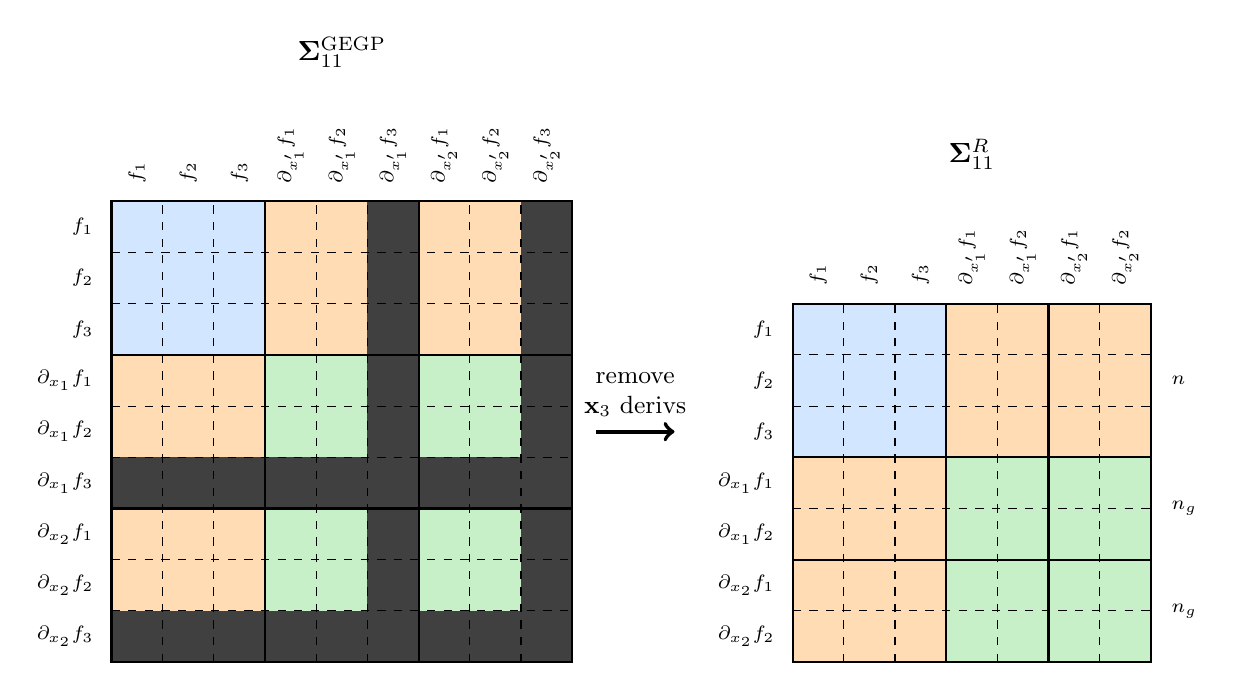
\begin{tikzpicture}
			\def\bw{0.65}
			\def\bh{0.65}

			% --- Left: GEGP 9x9 with blackout ---
			% Block structure: 3 block rows/cols (f, dx1, dx2), each 3 entries wide
			% Blackout: row/col 5 (dx1 for x3) and row/col 8 (dx2 for x3)

			% ff block
			\fill[ffblock] (0, 6*\bh) rectangle (3*\bw, 9*\bh);
			% f-dx1 block
			\fill[fdblock] (3*\bw, 6*\bh) rectangle (6*\bw, 9*\bh);
			\fill[black!75] (5*\bw, 6*\bh) rectangle (6*\bw, 9*\bh);
			% f-dx2 block
			\fill[fdblock] (6*\bw, 6*\bh) rectangle (9*\bw, 9*\bh);
			\fill[black!75] (8*\bw, 6*\bh) rectangle (9*\bw, 9*\bh);
			% dx1-f block
			\fill[fdblock] (0, 3*\bh) rectangle (3*\bw, 6*\bh);
			\fill[black!75] (0, 3*\bh) rectangle (3*\bw, 4*\bh);
			% dx1-dx1 block
			\fill[ddblock] (3*\bw, 3*\bh) rectangle (6*\bw, 6*\bh);
			\fill[black!75] (3*\bw, 3*\bh) rectangle (6*\bw, 4*\bh);
			\fill[black!75] (5*\bw, 3*\bh) rectangle (6*\bw, 6*\bh);
			% dx1-dx2 block
			\fill[ddblock] (6*\bw, 3*\bh) rectangle (9*\bw, 6*\bh);
			\fill[black!75] (6*\bw, 3*\bh) rectangle (9*\bw, 4*\bh);
			\fill[black!75] (8*\bw, 3*\bh) rectangle (9*\bw, 6*\bh);
			% dx2-f block
			\fill[fdblock] (0, 0) rectangle (3*\bw, 3*\bh);
			\fill[black!75] (0, 0) rectangle (3*\bw, 1*\bh);
			% dx2-dx1 block
			\fill[ddblock] (3*\bw, 0) rectangle (6*\bw, 3*\bh);
			\fill[black!75] (3*\bw, 0) rectangle (6*\bw, 1*\bh);
			\fill[black!75] (5*\bw, 0) rectangle (6*\bw, 3*\bh);
			% dx2-dx2 block
			\fill[ddblock] (6*\bw, 0) rectangle (9*\bw, 3*\bh);
			\fill[black!75] (6*\bw, 0) rectangle (9*\bw, 1*\bh);
			\fill[black!75] (8*\bw, 0) rectangle (9*\bw, 3*\bh);

			% Grid - outer
			\draw[black, thick] (0,0) rectangle (9*\bw, 9*\bh);
			% Block separators
			\draw[black, thick] (3*\bw, 0) -- (3*\bw, 9*\bh);
			\draw[black, thick] (6*\bw, 0) -- (6*\bw, 9*\bh);
			\draw[black, thick] (0, 3*\bh) -- (9*\bw, 3*\bh);
			\draw[black, thick] (0, 6*\bh) -- (9*\bw, 6*\bh);
			% Sub-grid within blocks (dashed)
			\foreach \i in {1,2,4,5,7,8} {
				\draw[black, thin, dashed] (\i*\bw, 0) -- (\i*\bw, 9*\bh);
				\draw[black, thin, dashed] (0, \i*\bh) -- (9*\bw, \i*\bh);
			}

			% Row labels
			\node[left=3pt, font=\scriptsize] at (0, 8.5*\bh) {$f_1$};
			\node[left=3pt, font=\scriptsize] at (0, 7.5*\bh) {$f_2$};
			\node[left=3pt, font=\scriptsize] at (0, 6.5*\bh) {$f_3$};
			\node[left=3pt, font=\scriptsize] at (0, 5.5*\bh) {$\partial_{x_1} f_1$};
			\node[left=3pt, font=\scriptsize] at (0, 4.5*\bh) {$\partial_{x_1} f_2$};
			\node[left=3pt, font=\scriptsize] at (0, 3.5*\bh) {$\partial_{x_1} f_3$};
			\node[left=3pt, font=\scriptsize] at (0, 2.5*\bh) {$\partial_{x_2} f_1$};
			\node[left=3pt, font=\scriptsize] at (0, 1.5*\bh) {$\partial_{x_2} f_2$};
			\node[left=3pt, font=\scriptsize] at (0, 0.5*\bh) {$\partial_{x_2} f_3$};

			% Column labels (with primes, rotated vertical)
			\node[above=3pt, font=\scriptsize, rotate=90, anchor=west] at (0.5*\bw, 9*\bh) {$f_1$};
			\node[above=3pt, font=\scriptsize, rotate=90, anchor=west] at (1.5*\bw, 9*\bh) {$f_2$};
			\node[above=3pt, font=\scriptsize, rotate=90, anchor=west] at (2.5*\bw, 9*\bh) {$f_3$};
			\node[above=3pt, font=\scriptsize, rotate=90, anchor=west] at (3.5*\bw, 9*\bh) {$\partial_{x_1'} f_1$};
			\node[above=3pt, font=\scriptsize, rotate=90, anchor=west] at (4.5*\bw, 9*\bh) {$\partial_{x_1'} f_2$};
			\node[above=3pt, font=\scriptsize, rotate=90, anchor=west] at (5.5*\bw, 9*\bh) {$\partial_{x_1'} f_3$};
			\node[above=3pt, font=\scriptsize, rotate=90, anchor=west] at (6.5*\bw, 9*\bh) {$\partial_{x_2'} f_1$};
			\node[above=3pt, font=\scriptsize, rotate=90, anchor=west] at (7.5*\bw, 9*\bh) {$\partial_{x_2'} f_2$};
			\node[above=3pt, font=\scriptsize, rotate=90, anchor=west] at (8.5*\bw, 9*\bh) {$\partial_{x_2'} f_3$};

			% Title
			\node[above=45pt, font=\normalsize] at (4.5*\bw, 9*\bh) {$\boldsymbol{\Sigma}_{11}^{\text{GEGP}}$};

			% --- Arrow ---
			\pgfmathsetmacro{\arrowstart}{9*\bw+0.3}
			\pgfmathsetmacro{\arrowend}{9*\bw+1.3}
			\pgfmathsetmacro{\arrowmid}{(\arrowstart+\arrowend)/2}
			\draw[->, line width=1.5pt] (\arrowstart, 4.5*\bh) -- (\arrowend, 4.5*\bh);
			\node[above=2pt, font=\small, align=center] at (\arrowmid, 4.5*\bh) {remove\\$\mathbf{x}_3$ derivs};

			% --- Right: RdGEGP 7x7 matrix ---
			\pgfmathsetmacro{\rx}{9*\bw+2.8}
			\def\rbw{0.65}
			\def\rbh{0.65}

			% ff block (3x3)
			\fill[ffblock] (\rx, 4*\rbh) rectangle (\rx+3*\rbw, 7*\rbh);
			% f-dx1 block (3x2)
			\fill[fdblock] (\rx+3*\rbw, 4*\rbh) rectangle (\rx+5*\rbw, 7*\rbh);
			% f-dx2 block (3x2)
			\fill[fdblock] (\rx+5*\rbw, 4*\rbh) rectangle (\rx+7*\rbw, 7*\rbh);
			% dx1-f block (2x3)
			\fill[fdblock] (\rx, 2*\rbh) rectangle (\rx+3*\rbw, 4*\rbh);
			% dx1-dx1 block (2x2)
			\fill[ddblock] (\rx+3*\rbw, 2*\rbh) rectangle (\rx+5*\rbw, 4*\rbh);
			% dx1-dx2 block (2x2)
			\fill[ddblock] (\rx+5*\rbw, 2*\rbh) rectangle (\rx+7*\rbw, 4*\rbh);
			% dx2-f block (2x3)
			\fill[fdblock] (\rx, 0) rectangle (\rx+3*\rbw, 2*\rbh);
			% dx2-dx1 block (2x2)
			\fill[ddblock] (\rx+3*\rbw, 0) rectangle (\rx+5*\rbw, 2*\rbh);
			% dx2-dx2 block (2x2)
			\fill[ddblock] (\rx+5*\rbw, 0) rectangle (\rx+7*\rbw, 2*\rbh);

			% Grid - outer
			\draw[black, thick] (\rx, 0) rectangle (\rx+7*\rbw, 7*\rbh);
			% Block separators
			\draw[black, thick] (\rx+3*\rbw, 0) -- (\rx+3*\rbw, 7*\rbh);
			\draw[black, thick] (\rx+5*\rbw, 0) -- (\rx+5*\rbw, 7*\rbh);
			\draw[black, thick] (\rx, 4*\rbh) -- (\rx+7*\rbw, 4*\rbh);
			\draw[black, thick] (\rx, 2*\rbh) -- (\rx+7*\rbw, 2*\rbh);
			% Sub-grid (dashed)
			\draw[black, thin, dashed] (\rx+1*\rbw, 0) -- (\rx+1*\rbw, 7*\rbh);
			\draw[black, thin, dashed] (\rx+2*\rbw, 0) -- (\rx+2*\rbw, 7*\rbh);
			\draw[black, thin, dashed] (\rx+4*\rbw, 0) -- (\rx+4*\rbw, 7*\rbh);
			\draw[black, thin, dashed] (\rx+6*\rbw, 0) -- (\rx+6*\rbw, 7*\rbh);
			\draw[black, thin, dashed] (\rx, 5*\rbh) -- (\rx+7*\rbw, 5*\rbh);
			\draw[black, thin, dashed] (\rx, 6*\rbh) -- (\rx+7*\rbw, 6*\rbh);
			\draw[black, thin, dashed] (\rx, 3*\rbh) -- (\rx+7*\rbw, 3*\rbh);
			\draw[black, thin, dashed] (\rx, 1*\rbh) -- (\rx+7*\rbw, 1*\rbh);

			% Row labels
			\node[left=3pt, font=\scriptsize] at (\rx, 6.5*\rbh) {$f_1$};
			\node[left=3pt, font=\scriptsize] at (\rx, 5.5*\rbh) {$f_2$};
			\node[left=3pt, font=\scriptsize] at (\rx, 4.5*\rbh) {$f_3$};
			\node[left=3pt, font=\scriptsize] at (\rx, 3.5*\rbh) {$\partial_{x_1} f_1$};
			\node[left=3pt, font=\scriptsize] at (\rx, 2.5*\rbh) {$\partial_{x_1} f_2$};
			\node[left=3pt, font=\scriptsize] at (\rx, 1.5*\rbh) {$\partial_{x_2} f_1$};
			\node[left=3pt, font=\scriptsize] at (\rx, 0.5*\rbh) {$\partial_{x_2} f_2$};

			% Column labels (with primes, rotated vertical)
			\node[above=3pt, font=\scriptsize, rotate=90, anchor=west] at (\rx+0.5*\rbw, 7*\rbh) {$f_1$};
			\node[above=3pt, font=\scriptsize, rotate=90, anchor=west] at (\rx+1.5*\rbw, 7*\rbh) {$f_2$};
			\node[above=3pt, font=\scriptsize, rotate=90, anchor=west] at (\rx+2.5*\rbw, 7*\rbh) {$f_3$};
			\node[above=3pt, font=\scriptsize, rotate=90, anchor=west] at (\rx+3.5*\rbw, 7*\rbh) {$\partial_{x_1'} f_1$};
			\node[above=3pt, font=\scriptsize, rotate=90, anchor=west] at (\rx+4.5*\rbw, 7*\rbh) {$\partial_{x_1'} f_2$};
			\node[above=3pt, font=\scriptsize, rotate=90, anchor=west] at (\rx+5.5*\rbw, 7*\rbh) {$\partial_{x_2'} f_1$};
			\node[above=3pt, font=\scriptsize, rotate=90, anchor=west] at (\rx+6.5*\rbw, 7*\rbh) {$\partial_{x_2'} f_2$};

			% Block dimension annotations (right side)
			\node[right=4pt, font=\scriptsize] at (\rx+7*\rbw, 5.5*\rbh) {$n$};
			\node[right=4pt, font=\scriptsize] at (\rx+7*\rbw, 3.0*\rbh) {$n_g$};
			\node[right=4pt, font=\scriptsize] at (\rx+7*\rbw, 1.0*\rbh) {$n_g$};

			% Title
			\node[above=45pt, font=\normalsize] at (\rx+3.5*\rbw, 7*\rbh) {$\boldsymbol{\Sigma}_{11}^{R}$};
		\end{tikzpicture}
		\caption{Covariance matrix reduction: the excluded derivative rows and columns for the non-gradient point $\mathbf{x}_3$ (black) are removed, reducing $\boldsymbol{\Sigma}_{11}^{\text{GEGP}}$ ($9 \times 9$) to $\boldsymbol{\Sigma}_{11}^{R}$ ($7 \times 7$). Note the asymmetric block structure: function blocks span all $n = 3$ points, while derivative blocks span only $n_g = 2$ gradient-observed points.}
		\label{fig:rdgegp_cov_reduction}
	\end{subfigure}

	\vspace{8pt}
	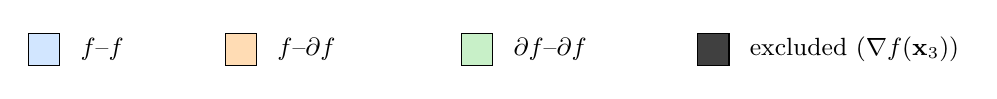
\begin{tikzpicture}
		\fill[ffblock] (0,0) rectangle (0.4, 0.4);
		\draw[black] (0,0) rectangle (0.4, 0.4);
		\node[right=4pt, font=\small] at (0.4, 0.2) {$f$--$f$};

		\fill[fdblock] (2.5,0) rectangle (2.9, 0.4);
		\draw[black] (2.5,0) rectangle (2.9, 0.4);
		\node[right=4pt, font=\small] at (2.9, 0.2) {$f$--$\partial f$};

		\fill[ddblock] (5.5,0) rectangle (5.9, 0.4);
		\draw[black] (5.5,0) rectangle (5.9, 0.4);
		\node[right=4pt, font=\small] at (5.9, 0.2) {$\partial f$--$\partial f$};

		\fill[black!75] (8.5,0) rectangle (8.9, 0.4);
		\draw[black] (8.5,0) rectangle (8.9, 0.4);
		\node[right=4pt, font=\small] at (8.9, 0.2) {excluded ($\nabla f(\mathbf{x}_3)$)};
	\end{tikzpicture}

	\caption{Reduction from GEGP to RdGEGP for $d = 2$, $n = 3$, $n_g = 2$ (gradients available at $\mathbf{x}_1$, $\mathbf{x}_2$ only). Unlike PGEGP, which removes entire block rows/columns (corresponding to derivative dimensions), RdGEGP removes individual rows/columns within each derivative block (corresponding to specific training points).}
	\label{fig:rdgegp_structure_2d}
\end{figure}

\subsubsection{Selective Derivative Predictions at Test Locations}
\label{subsubsec:rdgegp_selective_pred}

The same principles for selective derivative predictions described in Section~\ref{subsec:selective_deriv_pred} apply to the RdGEGP: predictions of any subset of function values and partial derivatives at test locations can be obtained by retaining the corresponding block columns in $\boldsymbol{\Sigma}^{R}_{12}$ and the corresponding block rows and columns in $\boldsymbol{\Sigma}^{R}_{22}$, without modifying $\boldsymbol{\Sigma}^{R}_{11}$. In particular, the training-side asymmetry---where only $n_g$ of $n$ training points contribute gradient observations---does not restrict the derivative predictions available at test locations, since the test-side covariance blocks in Equation~\eqref{eqn:rdgegp_S12_full} include derivative columns for \emph{all} test points $\mathbf{X}_*$. This is analogous to the PGEGP (Section~\ref{subsec:pgegp}), where derivatives excluded during training can still be predicted at test locations.

\begin{remark}
	The RdGEGP is the single-submodel special case ($M = 1$) of the Weighted Gradient-Enhanced GP (WGEGP) presented in Section~\ref{subsec:wgegp}. When $n_g = n$ (all training points have gradient information), the RdGEGP recovers the full GEGP of Section~\ref{subsec:derivative_gps}. The WGEGP generalizes this by partitioning the full gradient dataset into $M$ disjoint sets and constructing $M$ separate RdGEGP submodels, each with its own subset of gradient-observed points, which are then combined through a weighted summation.
\end{remark}

\paragraph{Numerical example.}
Using the same test function and $5 \times 5$ training grid, the RdGEGP includes gradient information at only $n_g = 10$ of the $n = 25$ training points (red triangles in Figure~\ref{fig:rdgegp_example}), while function values are available at all points. The resulting covariance matrix has dimension $n + d \cdot n_g = 25 + 2 \cdot 10 = 45$, compared to $n(d + 1) = 75$ for the full GEGP. Figure~\ref{fig:rdgegp_example} shows that the predictions remain reasonable despite having gradients at less than half of the training locations. The predictive uncertainty is notably higher in regions far from the gradient-observed points, clearly reflecting the heterogeneous information content across the training set.

\begin{figure}[H]
	\centering
	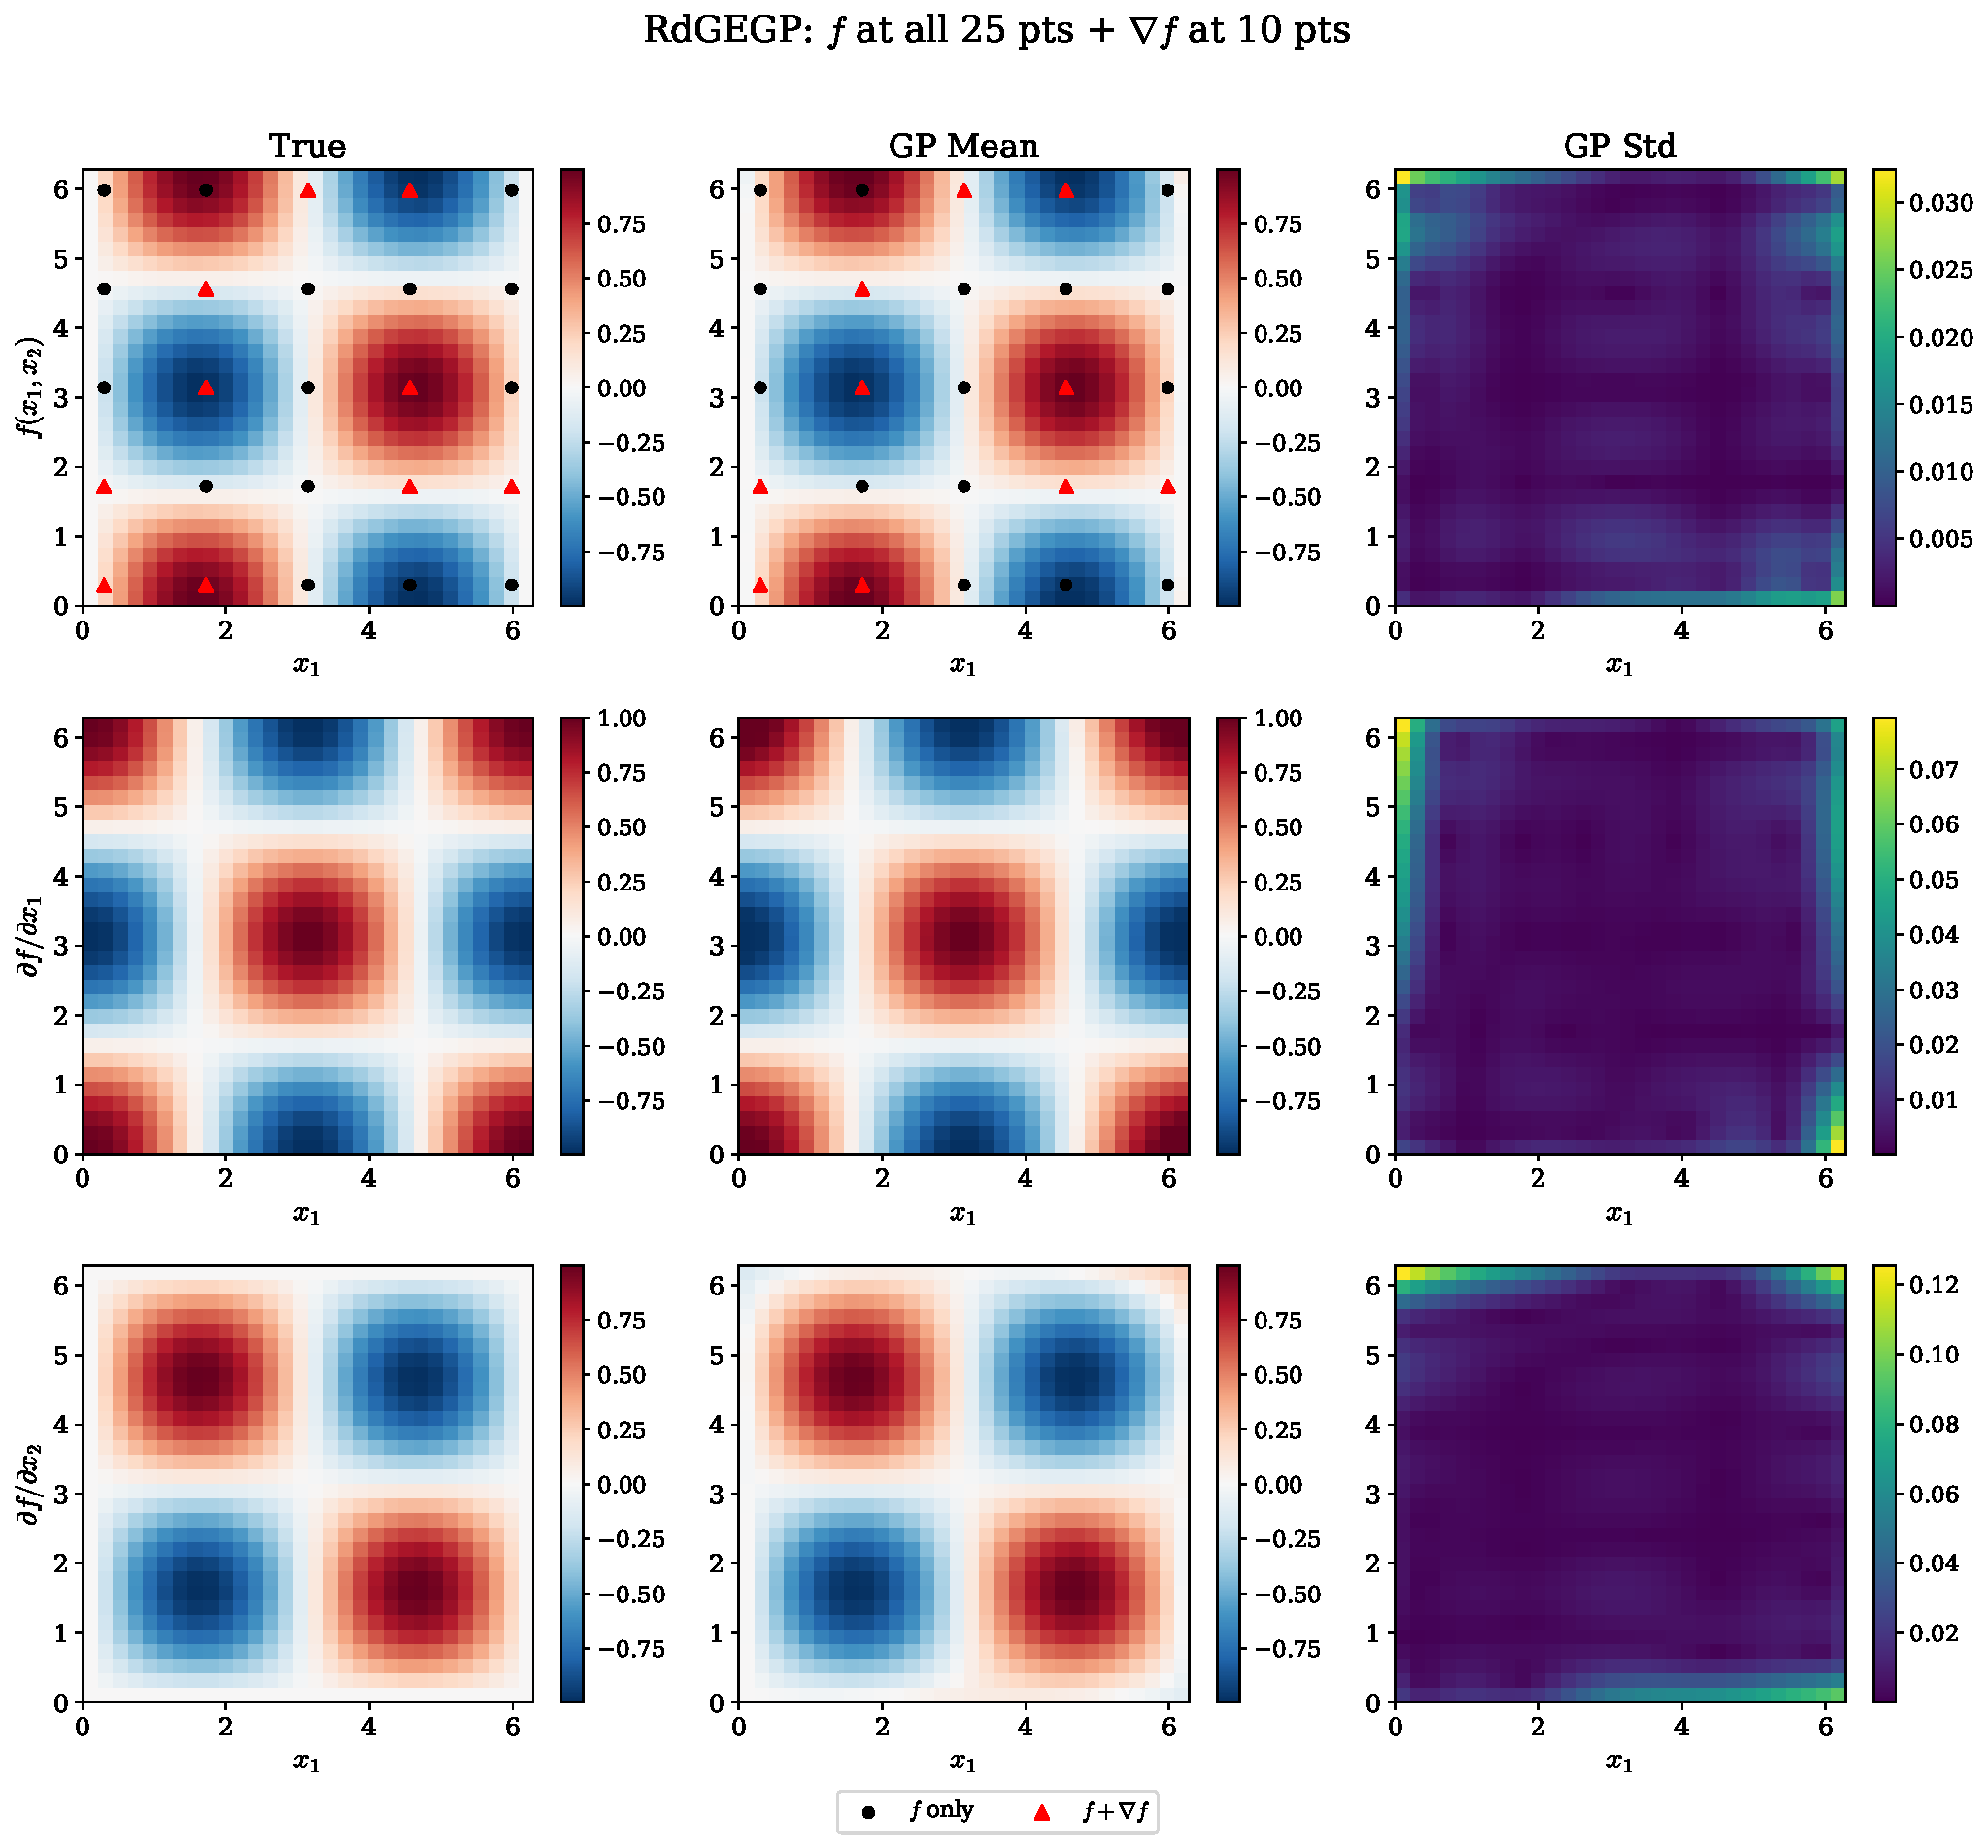
\includegraphics[width=\textwidth]{rdgegp_example.pdf}
	\caption{RdGEGP example on $f(x_1, x_2) = \sin(x_1)\cos(x_2)$ with $n = 25$ training points. Black circles denote function-only observations; red triangles denote locations where both function values and gradients are observed ($n_g = 10$). Rows show $f$, $\partial f / \partial x_1$, and $\partial f / \partial x_2$; columns show the true function, GP posterior mean, and posterior standard deviation.}
	\label{fig:rdgegp_example}
\end{figure}

%==============================================================================
\subsection{Weighted Gradient Enhanced Gaussian Processes}
\label{subsec:wgegp}
The Reduced Gradient-Enhanced GP (Section~\ref{subsec:rdgegp}) showed how to handle the case where only a subset of training points have gradient observations. The Weighted Gradient-Enhanced GP (WGEGP), referred to in the literature as Weighted Gradient-Enhanced Kriging (WGEK)~\cite{HanWeightedGEK, improved_gek}, extends this idea by decomposing the full gradient dataset into $M$ disjoint subsets, each defining an RdGEGP submodel. Rather than training a single GP on all derivative data, WGEGP constructs $M$ smaller submodels---each with the RdGEGP structure of Section~\ref{subsec:rdgegp}---and combines them through a weighted sum that preserves the full set of interpolation conditions. The key advantage is that each submodel operates on a much smaller correlation matrix, avoiding the computational cost of decomposing the full gradient-enhanced covariance matrix.

\subsubsection{Formulation}
\label{subsubsec:wgegp_formulation}

The WGEGP formulation begins with an observed training dataset $\mathcal{D}$ containing $n$ input-output pairs with gradients:
\begin{equation}
	\mathcal{D} = \left\{\mathbf{X}, f(\mathbf{X}), \nabla f(\mathbf{X})\right\} := \left\{(\mathbf{x}_i, f(\mathbf{x}_i), \nabla f(\mathbf{x}_i)) \mid i = 1, \ldots, n \right\}.
\end{equation}

The gradient information $\nabla f(\mathbf{X})$ is partitioned into $M \leq n$ disjoint sets:
\begin{align}
	D_1 & = \left\{\nabla f(\mathbf{x}_i) \mid  i = 1, \ldots, m_1\right\}, \nonumber \\
	D_2 &= \left\{\nabla f(\mathbf{x}_i) \mid  i = m_1 + 1, \ldots, m_2\right\}, \nonumber  \\
	& \vdots \nonumber  \\
	D_M & = \left\{\nabla f(\mathbf{x}_i) \mid  i = m_{M-1} + 1, \ldots, n\right\}, \nonumber  
\end{align}
where $0 < m_1 < m_2 < \cdots < m_{M-1} < n$ are cumulative partition boundaries. The training data for the $k^{\text{th}}$ submodel is then:
\begin{equation}
	\mathcal{D}_k = \left\{(\mathbf{x}_i, f(\mathbf{x}_i)) \mid i = 1, \ldots, n \right\} \cup D_k.
\end{equation}

That is, each submodel contains all $n$ function values but only the gradient information from partition $D_k$. Let $\mathcal{I}_k = \{i \mid \nabla f(\mathbf{x}_i) \in D_k\}$ denote the indices corresponding to partition $D_k$, let $n_k = |\mathcal{I}_k|$ denote the number of gradient-observed points in this partition, and let $\mathbf{X}_k = \{\mathbf{x}_i \mid i \in \mathcal{I}_k\}$ denote their locations. The observation vector for the $k^{\text{th}}$ submodel is augmented to include only these selected gradients:
\begin{equation}
	\label{eqn:wgek_aug_vector}
	\mathbf{y}^{(k)} = \begin{bmatrix}
		f(\mathbf{X}) \\
		\nabla f(\mathbf{X}_k)
	\end{bmatrix} \in \mathbb{R}^{n + d \cdot n_k}.
\end{equation}

For each submodel $k$, the joint distribution between the augmented training observations $\mathbf{y}^{(k)}$ and the test predictions is multivariate Gaussian:
\begin{equation}
	\label{eqn:wgek_joint_dist}
	\begin{pmatrix}
		\mathbf{y}^{(k)} \\
		\mathbf{y}^{(k)}_*
	\end{pmatrix}
	\sim \mathcal{N}\left(
	\mathbf{0},
	\begin{pmatrix}
		\boldsymbol{\Sigma}^{(k)}_{11} & \boldsymbol{\Sigma}^{(k)}_{12} \\
		\boldsymbol{\Sigma}^{(k)}_{21} & \boldsymbol{\Sigma}^{(k)}_{22}
	\end{pmatrix}
	\right),
\end{equation}
where $\mathbf{y}^{(k)}_*$ contains the test predictions (function values and, optionally, derivatives at test locations).

The training covariance block $\boldsymbol{\Sigma}^{(k)}_{11}$ is an $(n + d \cdot n_k) \times (n + d \cdot n_k)$ matrix:
\begin{equation}
	\label{eqn:wgek_S11}
	\boldsymbol{\Sigma}^{(k)}_{11} =
	\begin{pmatrix}
		K & \partial_{\mathbf{X}_k'} K \\
		\partial_{\mathbf{X}_k} K & \partial^2_{\mathbf{X}_k\,\mathbf{X}_k'} K
	\end{pmatrix}.
\end{equation}
This has the same asymmetric block structure as the RdGEGP (Section~\ref{subsec:rdgegp}), with $K$ being $n \times n$, the off-diagonal blocks $n \times d \cdot n_k$, and the lower-right block $d \cdot n_k \times d \cdot n_k$.

The full training-test covariance block, including derivative predictions at test points, is:
\begin{equation}
	\label{eqn:wgek_S12_full}
	\boldsymbol{\Sigma}^{(k)}_{12} =
	\begin{pmatrix}
		K & \partial_{\mathbf{X}_*'} K \\
		\partial_{\mathbf{X}_k} K & \partial^2_{\mathbf{X}_k\,\mathbf{X}_*'} K
	\end{pmatrix}.
\end{equation}
The posterior predictive distribution for the $k^{\text{th}}$ submodel follows the standard GP conditioning formula:
\begin{equation}
	\label{eqn:wgek_posterior}
	\begin{split}
		\boldsymbol{\mu}^{(k)}_{*} &= \boldsymbol{\Sigma}^{(k)}_{21} \left(\boldsymbol{\Sigma}^{(k)}_{11}\right)^{-1} \mathbf{y}^{(k)}, \\
		\boldsymbol{\Sigma}^{(k)}_{*} &=  \boldsymbol{\Sigma}^{(k)}_{22} - \boldsymbol{\Sigma}^{(k)}_{21} \left(\boldsymbol{\Sigma}^{(k)}_{11}\right)^{-1} \boldsymbol{\Sigma}^{(k)}_{12}.
	\end{split}
\end{equation}

Each submodel now provides a valid posterior predictive distribution, but these must be combined in a manner that preserves the interpolation conditions across all training data. By construction, each submodel prediction $\boldsymbol{\mu}_*^{(k)}$ exactly interpolates its training observations: $\boldsymbol{\mu}_*^{(k)}(\mathbf{x}_i) = f(\mathbf{x}_i)$ for all $i$, and $\nabla \boldsymbol{\mu}_*^{(k)}(\mathbf{x}_i) = \nabla f(\mathbf{x}_i)$ for $i \in \mathcal{I}_k$. The $M$ submodel predictions are then combined through a weighted summation to obtain the global prediction $\boldsymbol{\mu}_*$ at test locations $\mathbf{X}_*$:
\begin{equation}
	\label{eqn:wgek_weighted_prediction}
	\boldsymbol{\mu}_* = \sum_{k=1}^{M} w_k \boldsymbol{\mu}_*^{(k)},
\end{equation}
where $w_k: \mathbb{R}^d \to \mathbb{R}$ are weight functions. To ensure that the WGEGP predictor preserves these interpolation conditions globally (i.e., $\boldsymbol{\mu}_*(\mathbf{x}_i) = f(\mathbf{x}_i)$ for all training points), the weights must satisfy:
\begin{equation}
	\label{eqn:wgek_weight_constraints}
	\sum_{k=1}^{M} w_k(\mathbf{x}) = 1 \quad \forall \mathbf{x} \in \mathbb{R}^d,
\end{equation}
and
\begin{equation}
	w_k(\mathbf{x}_i) = \begin{cases}
		1 & \text{if } i \in \mathcal{I}_k, \\
		0 & \text{otherwise}.
	\end{cases}
\end{equation}

That is, at each training point $\mathbf{x}_i$, only the submodel containing that point's gradient information (submodel $k$ where $i \in \mathcal{I}_k$) contributes to the prediction, thereby ensuring that both function and derivative interpolation conditions are satisfied.

To compute the weight functions satisfying these constraints, the methodology outlined in~\cite{HanWeightedGEK} is followed. For a given test set $\mathbf{X}_*$, the weights are determined by solving the following constrained linear system:
\begin{equation}
	\label{eqn:wgek_weight_system}
	\begin{bmatrix}
		K(\mathbf{X}, \mathbf{X}') & \mathbf{1}_n \\
		\mathbf{1}_n^T & 0
	\end{bmatrix}
	\begin{bmatrix}
		\mathbf{W} \\
		\boldsymbol{\lambda}
	\end{bmatrix} =
	\begin{bmatrix}
		K(\mathbf{X}, \mathbf{X}_*)  \\
		\mathbf{1}_{n_*}^T
	\end{bmatrix},
\end{equation}
where:
\begin{itemize}
	\item $\mathbf{W} \in \mathbb{R}^{n \times n_*}$ contains weight contributions from each training point (rows) to each test point (columns)
	\item $\mathbf{1}_n \in \mathbb{R}^{n}$ is a vector of ones enforcing the partition-of-unity constraint
	\item $\boldsymbol{\lambda} \in \mathbb{R}^{1 \times n_*}$ contains Lagrange multipliers for each test point
	\item $\mathbf{1}_{n_*}^T$ is a row vector of $n_*$ ones
\end{itemize}

The submodel weight coefficients $w_k(\mathbf{x}_*^{(j)})$ for the $k$-th submodel at test point $\mathbf{x}_*^{(j)}$ are obtained by summing the weight contributions from all training points belonging to partition $\mathcal{I}_k$:
\begin{equation}
	\label{eqn:wgek_submodel_weights}
	w_k(\mathbf{x}_*^{(j)}) = \sum_{i \in \mathcal{I}_k} W_{ij}.
\end{equation}
The predictive variance is computed following~\cite{HanWeightedGEK} by weighting the submodel standard deviations:
\begin{equation}
	\label{eqn:wgek_weighted_variance}
	\left[\boldsymbol{\Sigma}_{*}\right]_{jj} = \left(\sum_{k=1}^{M} w_k(\mathbf{x}_*^{(j)}) \sqrt{\left[\boldsymbol{\Sigma}^{(k)}_{*}\right]_{jj}}\right)^2,
\end{equation}
where $\left[\boldsymbol{\Sigma}^{(k)}_{*}\right]_{jj}$ is the predictive variance from the $k$-th submodel at test point $\mathbf{x}_*^{(j)}$.

As with the previous models, the kernel hyperparameters $\boldsymbol{\psi}$ must be determined. Since the submodels represent different views of the same underlying random process, they share the same hyperparameters. For the $k^{\text{th}}$ submodel, the marginal log-likelihood (MLL) of the augmented observations $\mathbf{y}^{(k)}$ is:
\begin{equation}
	\label{eqn:wgek_mll}
	\log p(\mathbf{y}^{(k)}|\mathbf{X}, \boldsymbol{\psi}) = -\frac{1}{2} \left(\mathbf{y}^{(k)}\right)^\top \left(\boldsymbol{\Sigma}^{(k)}_{11}\right)^{-1} \mathbf{y}^{(k)} - \frac{1}{2}\log|\boldsymbol{\Sigma}^{(k)}_{11}| - \frac{n + d \cdot n_k}{2}\log 2\pi.
\end{equation}
Following~\cite{HanWeightedGEK}, the shared hyperparameters are determined by maximizing an aggregated log-likelihood function:
\begin{equation}
	\label{eqn:wgek_jll}
	\text{JLL}(\boldsymbol{\psi}) = \frac{1}{M}\sum_{k=1}^{M}\log p(\mathbf{y}^{(k)}|\mathbf{X}, \boldsymbol{\psi}).
\end{equation}
This uniform averaging provides a computationally efficient approximation to the full joint likelihood while ensuring all submodels contribute equally to the hyperparameter estimation. The optimal hyperparameters are obtained as:
\begin{equation}
	\label{eqn:wgek_optimal_psi}
	\boldsymbol{\psi}^* = \argmax_{\boldsymbol{\psi}} \text{JLL}(\boldsymbol{\psi}).
\end{equation}

This decomposition reduces the total training complexity from $\mathcal{O}((n(d+1))^3)$ for standard GEK to $\mathcal{O}\left(\sum_{k=1}^M (n + d \cdot n_k)^3\right)$ for WGEGP, providing substantial computational savings when the partitions distribute the gradient information appropriately. However, this computational efficiency comes at the cost of model accuracy. By partitioning the derivative data, WGEGP disrupts the derivative cross-correlation structure that full GEGP exploits. As the number of partitions $M$ increases, each submodel contains less derivative information, making the global predictor progressively less informative. The extreme case of $M = n$ (one gradient per submodel) provides maximum computational savings but minimal derivative cross-correlation information, resulting in the least accurate predictions. Conversely, reducing $M$ retains more of the derivative correlation structure, improving model accuracy at the expense of increased computational cost. Thus, the choice of $M$ represents a trade-off between computational efficiency and predictive fidelity.

To make this concrete, consider the same example used for the RdGEGP: a function of two variables ($d = 2$) with $n = 3$ training points, all of which now have gradient observations. The full GEGP augmented vector has dimension $n(d+1) = 9$. Suppose the gradient data is partitioned into $M = 3$ submodels, each containing the gradient at a single training point:
\begin{equation}
	D_1 = \{\nabla f(\mathbf{x}_1)\}, \quad D_2 = \{\nabla f(\mathbf{x}_2)\}, \quad D_3 = \{\nabla f(\mathbf{x}_3)\}.
\end{equation}
Each submodel $k$ has $\mathcal{I}_k = \{k\}$, $n_k = 1$, and $\mathbf{X}_k = \{\mathbf{x}_k\}$. All three submodels share the function values at all $n = 3$ points but each contains the gradient at only one point, giving augmented vectors of dimension $n + d \cdot n_k = 3 + 2 \cdot 1 = 5$:
\begin{equation}
	\label{eqn:wgegp_aug_vectors_2d}
	\mathbf{y}^{(1)} = \begin{bmatrix} f(\mathbf{x}_1) \\ f(\mathbf{x}_2) \\ f(\mathbf{x}_3) \\ \partial_{x_1} f(\mathbf{x}_1) \\ \partial_{x_2} f(\mathbf{x}_1) \end{bmatrix}, \quad
	\mathbf{y}^{(2)} = \begin{bmatrix} f(\mathbf{x}_1) \\ f(\mathbf{x}_2) \\ f(\mathbf{x}_3) \\ \partial_{x_1} f(\mathbf{x}_2) \\ \partial_{x_2} f(\mathbf{x}_2) \end{bmatrix}, \quad
	\mathbf{y}^{(3)} = \begin{bmatrix} f(\mathbf{x}_1) \\ f(\mathbf{x}_2) \\ f(\mathbf{x}_3) \\ \partial_{x_1} f(\mathbf{x}_3) \\ \partial_{x_2} f(\mathbf{x}_3) \end{bmatrix}.
\end{equation}
Each submodel is an RdGEGP (Section~\ref{subsec:rdgegp}) with $n_g = n_k = 1$. The corresponding training covariance block $\boldsymbol{\Sigma}^{(k)}_{11}$ is a $5 \times 5$ matrix with the asymmetric block structure:
\begin{equation}
	\label{eqn:wgegp_S11_2d}
	\boldsymbol{\Sigma}^{(k)}_{11} =
	\begin{pmatrix}
		K & \partial_{\mathbf{X}_k'} K \\
		\partial_{\mathbf{X}_k} K & \partial^2_{\mathbf{X}_k\,\mathbf{X}_k'} K
	\end{pmatrix}
	=
	\underbrace{\begin{pmatrix}
		\text{$3 \times 3$} & \text{$3 \times 2$} \\
		\text{$2 \times 3$} & \text{$2 \times 2$}
	\end{pmatrix}}_{\text{$5 \times 5$}},
\end{equation}
where the upper-left block captures covariances between function values at all $3$ training points, while the derivative blocks involve only the single gradient-observed point $\mathbf{x}_k$. Each submodel requires a Cholesky decomposition of this $5 \times 5$ matrix, giving a total cost of $3 \times \mathcal{O}(5^3)$ compared to $\mathcal{O}(9^3)$ for the full GEGP. The block structure of all three submodel covariance matrices is illustrated in Figure~\ref{fig:wgegp_cov_structure_2d}.

\begin{figure}[htbp]
	\centering
	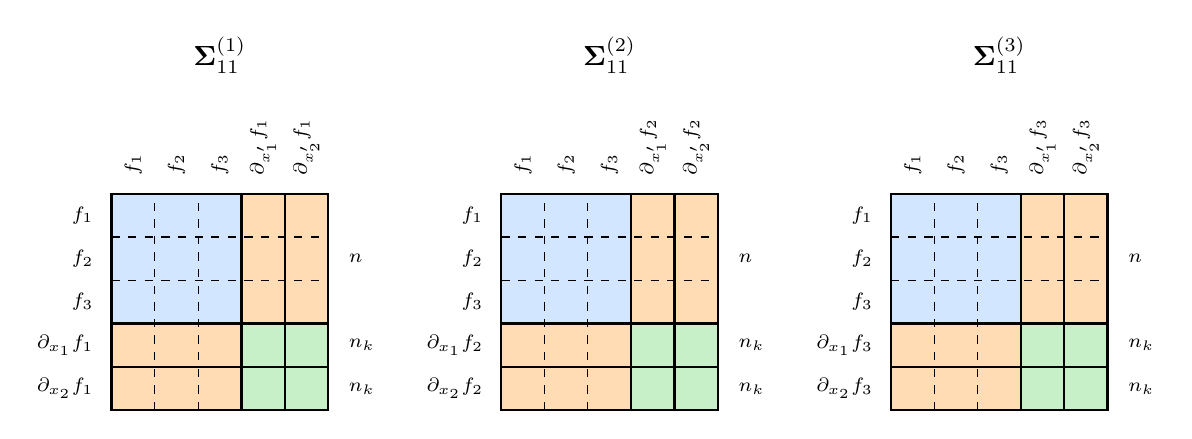
\begin{tikzpicture}
		\def\bw{0.55}
		\def\bh{0.55}
		\pgfmathsetmacro{\mtwo}{5*\bw + 2.2}
		\pgfmathsetmacro{\mthree}{2*(5*\bw + 2.2)}

		% ===== Submodel 1: Sigma_11^(1) =====
		% Block layout (bottom to top): dx2 (1 row), dx1 (1 row), f (3 rows)
		% Block layout (left to right): f (3 cols), dx1' (1 col), dx2' (1 col)

		% ff block (3x3)
		\fill[ffblock] (0, 2*\bh) rectangle (3*\bw, 5*\bh);
		% f-dx1 block (3x1)
		\fill[fdblock] (3*\bw, 2*\bh) rectangle (4*\bw, 5*\bh);
		% f-dx2 block (3x1)
		\fill[fdblock] (4*\bw, 2*\bh) rectangle (5*\bw, 5*\bh);
		% dx1-f block (1x3)
		\fill[fdblock] (0, 1*\bh) rectangle (3*\bw, 2*\bh);
		% dx1-dx1 block (1x1)
		\fill[ddblock] (3*\bw, 1*\bh) rectangle (4*\bw, 2*\bh);
		% dx1-dx2 block (1x1)
		\fill[ddblock] (4*\bw, 1*\bh) rectangle (5*\bw, 2*\bh);
		% dx2-f block (1x3)
		\fill[fdblock] (0, 0) rectangle (3*\bw, 1*\bh);
		% dx2-dx1 block (1x1)
		\fill[ddblock] (3*\bw, 0) rectangle (4*\bw, 1*\bh);
		% dx2-dx2 block (1x1)
		\fill[ddblock] (4*\bw, 0) rectangle (5*\bw, 1*\bh);

		% Grid - outer
		\draw[black, thick] (0, 0) rectangle (5*\bw, 5*\bh);
		% Block separators
		\draw[black, thick] (3*\bw, 0) -- (3*\bw, 5*\bh);
		\draw[black, thick] (4*\bw, 0) -- (4*\bw, 5*\bh);
		\draw[black, thick] (0, 2*\bh) -- (5*\bw, 2*\bh);
		\draw[black, thick] (0, 1*\bh) -- (5*\bw, 1*\bh);
		% Sub-grid (dashed) within f block
		\draw[black, thin, dashed] (1*\bw, 0) -- (1*\bw, 5*\bh);
		\draw[black, thin, dashed] (2*\bw, 0) -- (2*\bw, 5*\bh);
		\draw[black, thin, dashed] (0, 3*\bh) -- (5*\bw, 3*\bh);
		\draw[black, thin, dashed] (0, 4*\bh) -- (5*\bw, 4*\bh);

		% Row labels
		\node[left=3pt, font=\scriptsize] at (0, 4.5*\bh) {$f_1$};
		\node[left=3pt, font=\scriptsize] at (0, 3.5*\bh) {$f_2$};
		\node[left=3pt, font=\scriptsize] at (0, 2.5*\bh) {$f_3$};
		\node[left=3pt, font=\scriptsize] at (0, 1.5*\bh) {$\partial_{x_1} f_1$};
		\node[left=3pt, font=\scriptsize] at (0, 0.5*\bh) {$\partial_{x_2} f_1$};

		% Column labels (rotated)
		\node[above=3pt, font=\scriptsize, rotate=90, anchor=west] at (0.5*\bw, 5*\bh) {$f_1$};
		\node[above=3pt, font=\scriptsize, rotate=90, anchor=west] at (1.5*\bw, 5*\bh) {$f_2$};
		\node[above=3pt, font=\scriptsize, rotate=90, anchor=west] at (2.5*\bw, 5*\bh) {$f_3$};
		\node[above=3pt, font=\scriptsize, rotate=90, anchor=west] at (3.5*\bw, 5*\bh) {$\partial_{x_1'} f_1$};
		\node[above=3pt, font=\scriptsize, rotate=90, anchor=west] at (4.5*\bw, 5*\bh) {$\partial_{x_2'} f_1$};

		% Title
		\node[above=40pt, font=\normalsize] at (2.5*\bw, 5*\bh) {$\boldsymbol{\Sigma}_{11}^{(1)}$};

		% Dimension annotations
		\node[right=4pt, font=\scriptsize] at (5*\bw, 3.5*\bh) {$n$};
		\node[right=4pt, font=\scriptsize] at (5*\bw, 1.5*\bh) {$n_k$};
		\node[right=4pt, font=\scriptsize] at (5*\bw, 0.5*\bh) {$n_k$};

		% ===== Submodel 2: Sigma_11^(2) =====

		% ff block (3x3)
		\fill[ffblock] (\mtwo, 2*\bh) rectangle (\mtwo+3*\bw, 5*\bh);
		% f-dx1 block (3x1)
		\fill[fdblock] (\mtwo+3*\bw, 2*\bh) rectangle (\mtwo+4*\bw, 5*\bh);
		% f-dx2 block (3x1)
		\fill[fdblock] (\mtwo+4*\bw, 2*\bh) rectangle (\mtwo+5*\bw, 5*\bh);
		% dx1-f block (1x3)
		\fill[fdblock] (\mtwo, 1*\bh) rectangle (\mtwo+3*\bw, 2*\bh);
		% dx1-dx1 block (1x1)
		\fill[ddblock] (\mtwo+3*\bw, 1*\bh) rectangle (\mtwo+4*\bw, 2*\bh);
		% dx1-dx2 block (1x1)
		\fill[ddblock] (\mtwo+4*\bw, 1*\bh) rectangle (\mtwo+5*\bw, 2*\bh);
		% dx2-f block (1x3)
		\fill[fdblock] (\mtwo, 0) rectangle (\mtwo+3*\bw, 1*\bh);
		% dx2-dx1 block (1x1)
		\fill[ddblock] (\mtwo+3*\bw, 0) rectangle (\mtwo+4*\bw, 1*\bh);
		% dx2-dx2 block (1x1)
		\fill[ddblock] (\mtwo+4*\bw, 0) rectangle (\mtwo+5*\bw, 1*\bh);

		% Grid - outer
		\draw[black, thick] (\mtwo, 0) rectangle (\mtwo+5*\bw, 5*\bh);
		% Block separators
		\draw[black, thick] (\mtwo+3*\bw, 0) -- (\mtwo+3*\bw, 5*\bh);
		\draw[black, thick] (\mtwo+4*\bw, 0) -- (\mtwo+4*\bw, 5*\bh);
		\draw[black, thick] (\mtwo, 2*\bh) -- (\mtwo+5*\bw, 2*\bh);
		\draw[black, thick] (\mtwo, 1*\bh) -- (\mtwo+5*\bw, 1*\bh);
		% Sub-grid (dashed)
		\draw[black, thin, dashed] (\mtwo+1*\bw, 0) -- (\mtwo+1*\bw, 5*\bh);
		\draw[black, thin, dashed] (\mtwo+2*\bw, 0) -- (\mtwo+2*\bw, 5*\bh);
		\draw[black, thin, dashed] (\mtwo, 3*\bh) -- (\mtwo+5*\bw, 3*\bh);
		\draw[black, thin, dashed] (\mtwo, 4*\bh) -- (\mtwo+5*\bw, 4*\bh);

		% Row labels
		\node[left=3pt, font=\scriptsize] at (\mtwo, 4.5*\bh) {$f_1$};
		\node[left=3pt, font=\scriptsize] at (\mtwo, 3.5*\bh) {$f_2$};
		\node[left=3pt, font=\scriptsize] at (\mtwo, 2.5*\bh) {$f_3$};
		\node[left=3pt, font=\scriptsize] at (\mtwo, 1.5*\bh) {$\partial_{x_1} f_2$};
		\node[left=3pt, font=\scriptsize] at (\mtwo, 0.5*\bh) {$\partial_{x_2} f_2$};

		% Column labels (rotated)
		\node[above=3pt, font=\scriptsize, rotate=90, anchor=west] at (\mtwo+0.5*\bw, 5*\bh) {$f_1$};
		\node[above=3pt, font=\scriptsize, rotate=90, anchor=west] at (\mtwo+1.5*\bw, 5*\bh) {$f_2$};
		\node[above=3pt, font=\scriptsize, rotate=90, anchor=west] at (\mtwo+2.5*\bw, 5*\bh) {$f_3$};
		\node[above=3pt, font=\scriptsize, rotate=90, anchor=west] at (\mtwo+3.5*\bw, 5*\bh) {$\partial_{x_1'} f_2$};
		\node[above=3pt, font=\scriptsize, rotate=90, anchor=west] at (\mtwo+4.5*\bw, 5*\bh) {$\partial_{x_2'} f_2$};

		% Title
		\node[above=40pt, font=\normalsize] at (\mtwo+2.5*\bw, 5*\bh) {$\boldsymbol{\Sigma}_{11}^{(2)}$};

		% Dimension annotations
		\node[right=4pt, font=\scriptsize] at (\mtwo+5*\bw, 3.5*\bh) {$n$};
		\node[right=4pt, font=\scriptsize] at (\mtwo+5*\bw, 1.5*\bh) {$n_k$};
		\node[right=4pt, font=\scriptsize] at (\mtwo+5*\bw, 0.5*\bh) {$n_k$};

		% ===== Submodel 3: Sigma_11^(3) =====

		% ff block (3x3)
		\fill[ffblock] (\mthree, 2*\bh) rectangle (\mthree+3*\bw, 5*\bh);
		% f-dx1 block (3x1)
		\fill[fdblock] (\mthree+3*\bw, 2*\bh) rectangle (\mthree+4*\bw, 5*\bh);
		% f-dx2 block (3x1)
		\fill[fdblock] (\mthree+4*\bw, 2*\bh) rectangle (\mthree+5*\bw, 5*\bh);
		% dx1-f block (1x3)
		\fill[fdblock] (\mthree, 1*\bh) rectangle (\mthree+3*\bw, 2*\bh);
		% dx1-dx1 block (1x1)
		\fill[ddblock] (\mthree+3*\bw, 1*\bh) rectangle (\mthree+4*\bw, 2*\bh);
		% dx1-dx2 block (1x1)
		\fill[ddblock] (\mthree+4*\bw, 1*\bh) rectangle (\mthree+5*\bw, 2*\bh);
		% dx2-f block (1x3)
		\fill[fdblock] (\mthree, 0) rectangle (\mthree+3*\bw, 1*\bh);
		% dx2-dx1 block (1x1)
		\fill[ddblock] (\mthree+3*\bw, 0) rectangle (\mthree+4*\bw, 1*\bh);
		% dx2-dx2 block (1x1)
		\fill[ddblock] (\mthree+4*\bw, 0) rectangle (\mthree+5*\bw, 1*\bh);

		% Grid - outer
		\draw[black, thick] (\mthree, 0) rectangle (\mthree+5*\bw, 5*\bh);
		% Block separators
		\draw[black, thick] (\mthree+3*\bw, 0) -- (\mthree+3*\bw, 5*\bh);
		\draw[black, thick] (\mthree+4*\bw, 0) -- (\mthree+4*\bw, 5*\bh);
		\draw[black, thick] (\mthree, 2*\bh) -- (\mthree+5*\bw, 2*\bh);
		\draw[black, thick] (\mthree, 1*\bh) -- (\mthree+5*\bw, 1*\bh);
		% Sub-grid (dashed)
		\draw[black, thin, dashed] (\mthree+1*\bw, 0) -- (\mthree+1*\bw, 5*\bh);
		\draw[black, thin, dashed] (\mthree+2*\bw, 0) -- (\mthree+2*\bw, 5*\bh);
		\draw[black, thin, dashed] (\mthree, 3*\bh) -- (\mthree+5*\bw, 3*\bh);
		\draw[black, thin, dashed] (\mthree, 4*\bh) -- (\mthree+5*\bw, 4*\bh);

		% Row labels
		\node[left=3pt, font=\scriptsize] at (\mthree, 4.5*\bh) {$f_1$};
		\node[left=3pt, font=\scriptsize] at (\mthree, 3.5*\bh) {$f_2$};
		\node[left=3pt, font=\scriptsize] at (\mthree, 2.5*\bh) {$f_3$};
		\node[left=3pt, font=\scriptsize] at (\mthree, 1.5*\bh) {$\partial_{x_1} f_3$};
		\node[left=3pt, font=\scriptsize] at (\mthree, 0.5*\bh) {$\partial_{x_2} f_3$};

		% Column labels (rotated)
		\node[above=3pt, font=\scriptsize, rotate=90, anchor=west] at (\mthree+0.5*\bw, 5*\bh) {$f_1$};
		\node[above=3pt, font=\scriptsize, rotate=90, anchor=west] at (\mthree+1.5*\bw, 5*\bh) {$f_2$};
		\node[above=3pt, font=\scriptsize, rotate=90, anchor=west] at (\mthree+2.5*\bw, 5*\bh) {$f_3$};
		\node[above=3pt, font=\scriptsize, rotate=90, anchor=west] at (\mthree+3.5*\bw, 5*\bh) {$\partial_{x_1'} f_3$};
		\node[above=3pt, font=\scriptsize, rotate=90, anchor=west] at (\mthree+4.5*\bw, 5*\bh) {$\partial_{x_2'} f_3$};

		% Title
		\node[above=40pt, font=\normalsize] at (\mthree+2.5*\bw, 5*\bh) {$\boldsymbol{\Sigma}_{11}^{(3)}$};

		% Dimension annotations
		\node[right=4pt, font=\scriptsize] at (\mthree+5*\bw, 3.5*\bh) {$n$};
		\node[right=4pt, font=\scriptsize] at (\mthree+5*\bw, 1.5*\bh) {$n_k$};
		\node[right=4pt, font=\scriptsize] at (\mthree+5*\bw, 0.5*\bh) {$n_k$};
	\end{tikzpicture}

	\vspace{8pt}
	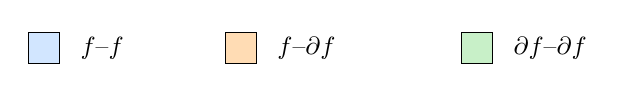
\begin{tikzpicture}
		\fill[ffblock] (0,0) rectangle (0.4, 0.4);
		\draw[black] (0,0) rectangle (0.4, 0.4);
		\node[right=4pt, font=\small] at (0.4, 0.2) {$f$--$f$};

		\fill[fdblock] (2.5,0) rectangle (2.9, 0.4);
		\draw[black] (2.5,0) rectangle (2.9, 0.4);
		\node[right=4pt, font=\small] at (2.9, 0.2) {$f$--$\partial f$};

		\fill[ddblock] (5.5,0) rectangle (5.9, 0.4);
		\draw[black] (5.5,0) rectangle (5.9, 0.4);
		\node[right=4pt, font=\small] at (5.9, 0.2) {$\partial f$--$\partial f$};
	\end{tikzpicture}

	\caption{Training covariance structure for the three WGEGP submodels with $d = 2$, $n = 3$, $M = 3$ ($n_k = 1$ for all $k$). Each $5 \times 5$ matrix $\boldsymbol{\Sigma}_{11}^{(k)}$ shares the same $3 \times 3$ function-function block (upper left) but differs in which training point contributes the gradient entries. Compare with the full $9 \times 9$ GEGP matrix in Figure~\ref{fig:rdgegp_cov_reduction}.}
	\label{fig:wgegp_cov_structure_2d}
\end{figure}

\paragraph{Numerical example.}
Using the same test function and training grid, the WGEGP partitions the 25 training points into $M = 2$ disjoint submodels, each receiving gradient information from approximately half of the points. Each submodel's covariance matrix has dimension $n + d \cdot n_k \approx 25 + 2 \cdot 12 = 49$, compared to the full GEGP matrix of dimension $75$. Since the Cholesky decomposition cost scales cubically, this roughly halves the per-submodel cost and avoids factoring the full $75 \times 75$ matrix. Figure~\ref{fig:wgegp_example} shows that the WGEGP predictions closely approximate those of the full GEGP (Figure~\ref{fig:gegp_example}), demonstrating that the weighted combination of submodels preserves prediction quality while reducing computational cost.

\begin{figure}[H]
	\centering
	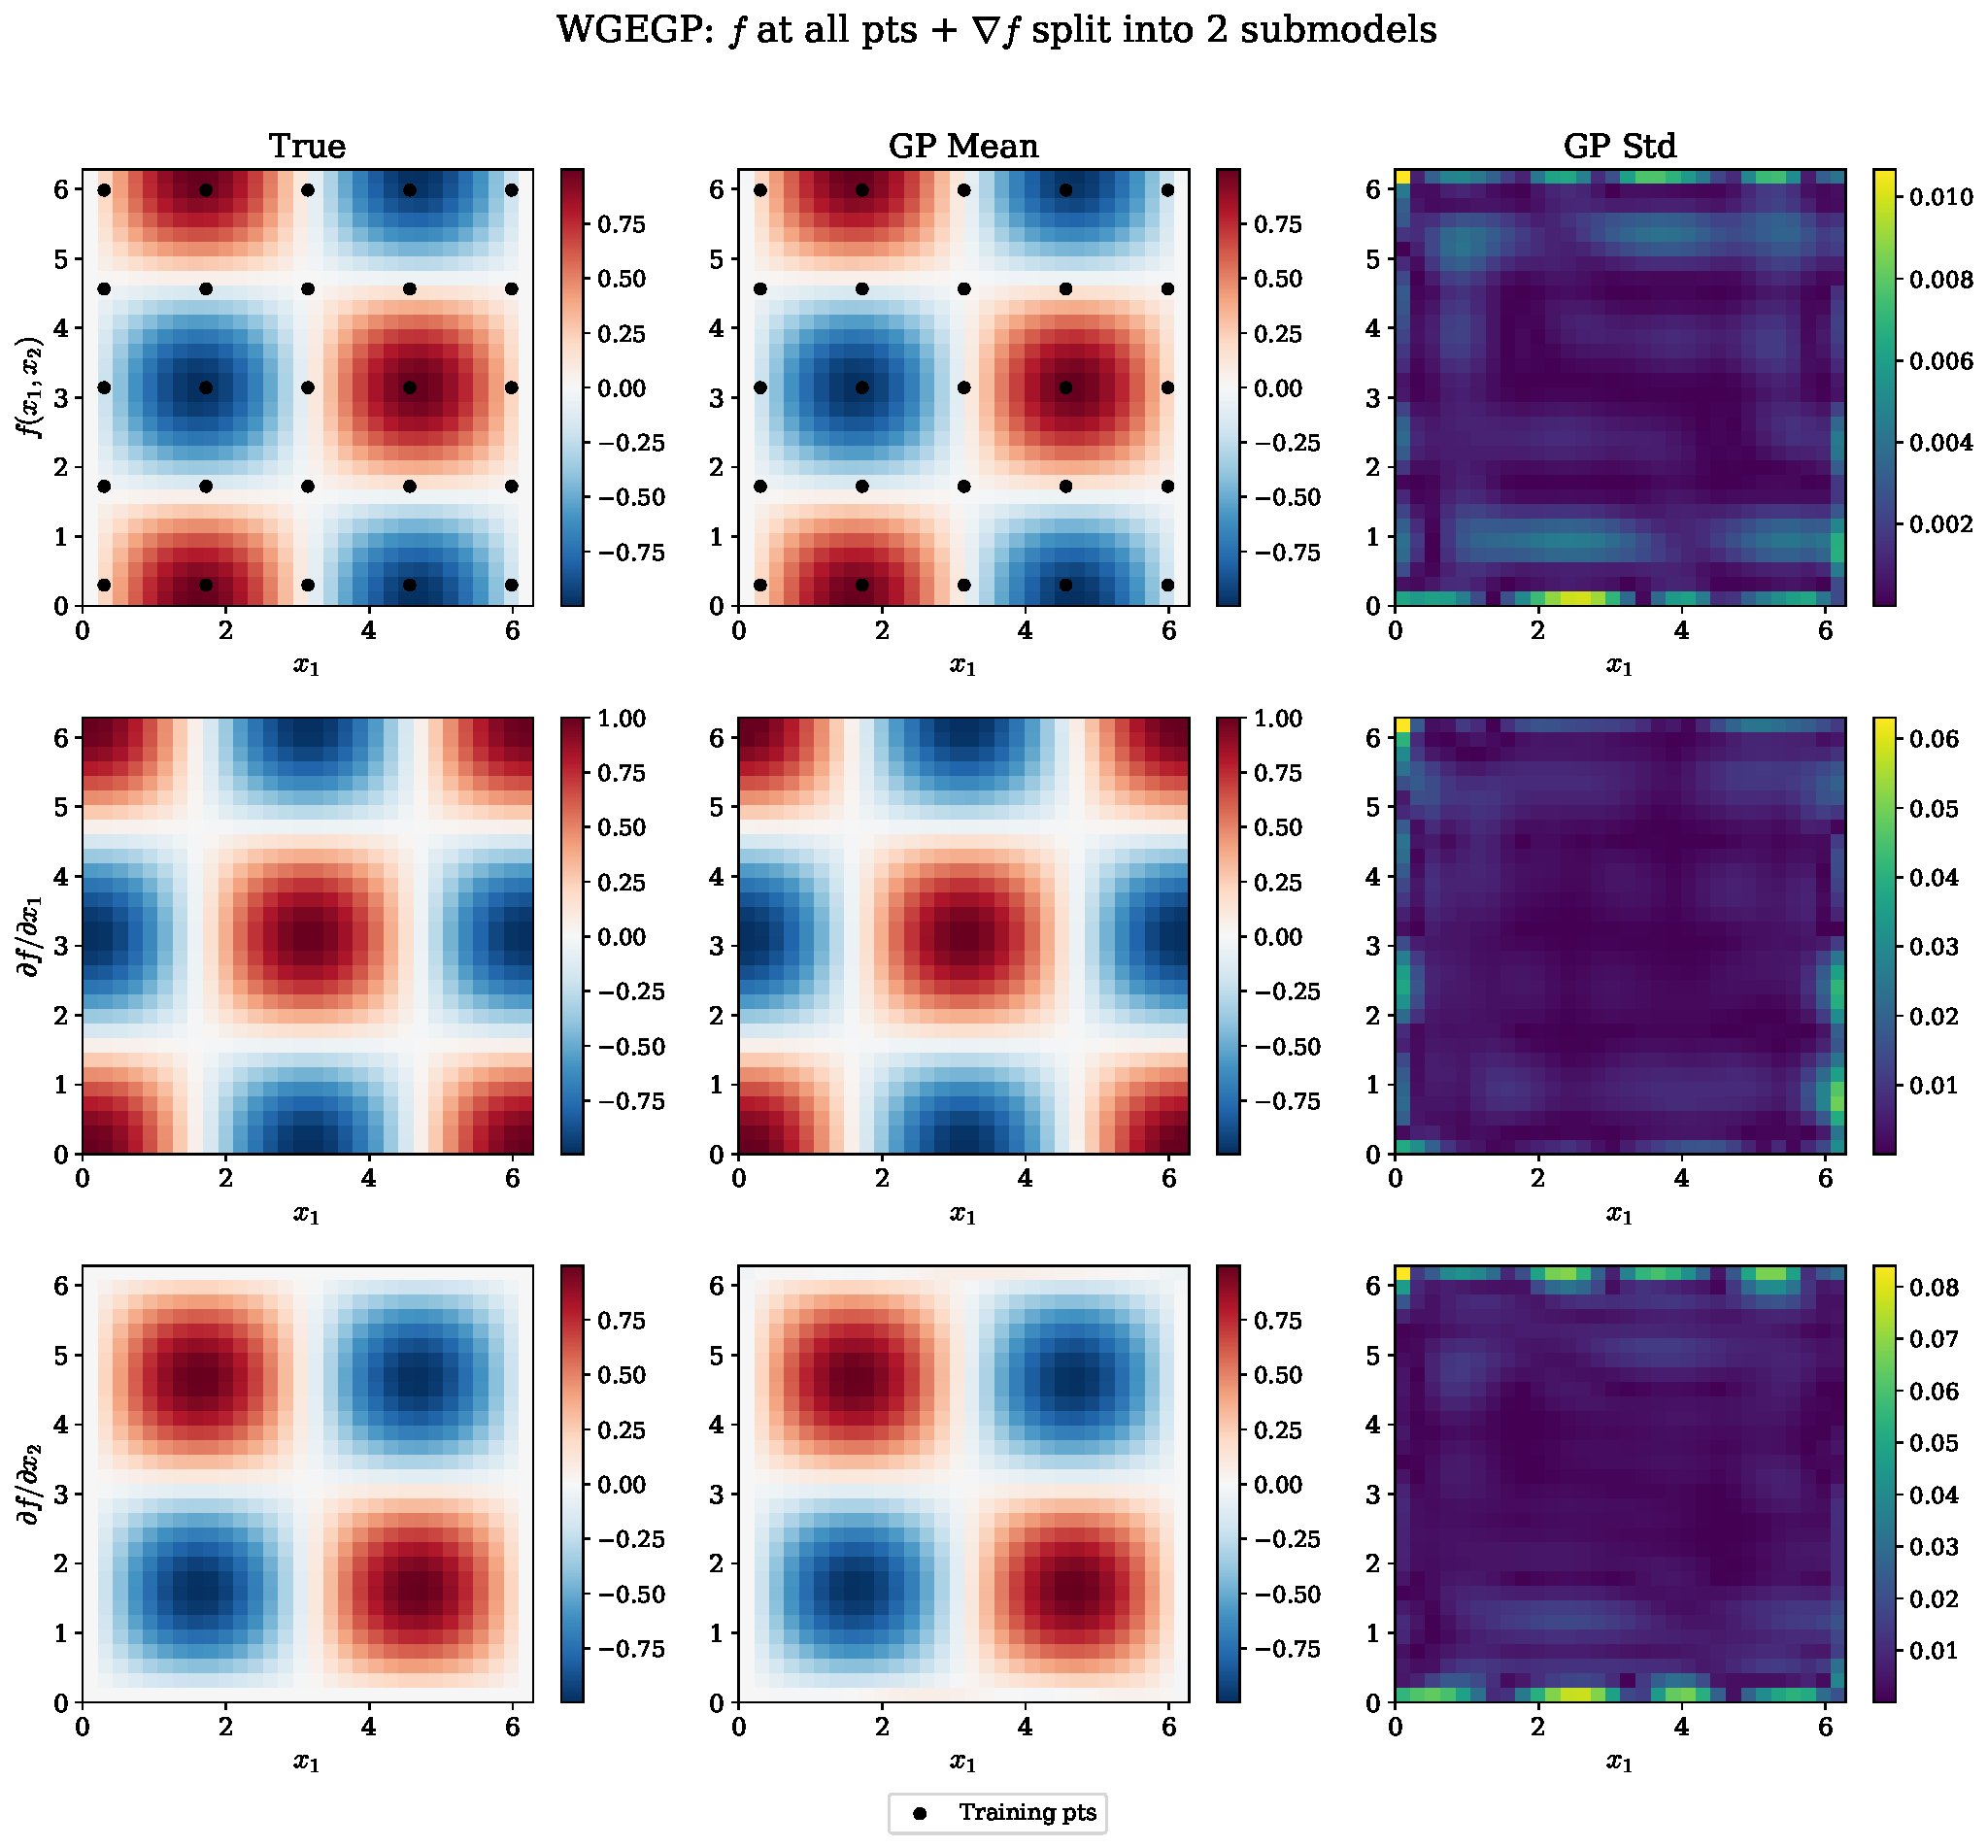
\includegraphics[width=\textwidth]{wgegp_example.pdf}
	\caption{WGEGP example on $f(x_1, x_2) = \sin(x_1)\cos(x_2)$ with $n = 25$ training points and gradient observations split into $M = 2$ disjoint submodels. Each submodel uses all function values but only its assigned subset of gradients. Rows show $f$, $\partial f / \partial x_1$, and $\partial f / \partial x_2$; columns show the true function, GP posterior mean, and posterior standard deviation.}
	\label{fig:wgegp_example}
\end{figure}

\subsubsection{Selective Derivative Predictions at Test Locations}
\label{subsubsec:wgegp_selective_pred}

The same principles for selective derivative predictions described in Section~\ref{subsec:selective_deriv_pred} apply to each WGEGP submodel. Since each submodel is an RdGEGP (Section~\ref{subsec:rdgegp}), predicting derivatives at test locations requires that the submodel's cross-covariance block $\boldsymbol{\Sigma}_{12}^{(k)}$ include the corresponding derivative columns and the test covariance block $\boldsymbol{\Sigma}_{22}^{(k)}$ include the corresponding derivative rows and columns, following the full form given in Equation~\eqref{eqn:wgek_S12_full}. When only function values are needed at test locations, the blocks simplify:
\begin{equation}
	\boldsymbol{\Sigma}_{12}^{(k)} \;\longrightarrow\;
	\begin{pmatrix}
		K \\
		\partial_{\mathbf{X}_k} K
	\end{pmatrix}, \quad \text{and} \quad
	\boldsymbol{\Sigma}_{22}^{(k)} \;\longrightarrow\; K.
\end{equation}
Returning to the $d = 2$, $n = 3$, $M = 3$ example above, suppose we wish to predict function values and full gradients at a set of test points $\mathbf{X}_*$. Each submodel's cross-covariance block $\boldsymbol{\Sigma}_{12}^{(k)}$ must then include derivative columns for all test points:
\begin{equation}
	\label{eqn:wgegp_S12_2d}
	\boldsymbol{\Sigma}_{12}^{(k)} =
	\begin{pmatrix}
		K & \partial_{\mathbf{X}_*'} K \\
		\partial_{\mathbf{X}_k} K & \partial^2_{\mathbf{X}_k\,\mathbf{X}_*'} K
	\end{pmatrix}
	=
	\underbrace{\begin{pmatrix}
		\text{$3 \times n_*$} & \text{$3 \times 2n_*$} \\
		\text{$2 \times n_*$} & \text{$2 \times 2n_*$}
	\end{pmatrix}}_{\text{$5 \times 3n_*$}},
\end{equation}
where $n_* = |\mathbf{X}_*|$. The derivative columns span all test points $\mathbf{X}_*$, regardless of which single training point $\mathbf{x}_k$ contributed gradient data to submodel $k$. Since each submodel prediction $\boldsymbol{\mu}_*^{(k)}$ can include derivative predictions, the weighted combination in Equation~\eqref{eqn:wgek_weighted_prediction} preserves this capability for the global predictor $\boldsymbol{\mu}_*$.

% =======================
% General Note on Noise
% =======================
\paragraph{Note on Observation Noise}
\label{par:gp_noise}
In practice, it is typical that the observed outputs are contaminated with
independent Gaussian noise, so that
\[
y_i = f(\mathbf{x}_i) + \epsilon_i,
\quad \epsilon_i \sim \mathcal{N}(0, \sigma_n^2).
\]
Using the block notation $\Sigma_{ij}$ for covariance matrices, where
$\Sigma_{11}$ denotes the covariance of the training outputs with themselves,
the presence of noise modifies only this block:
\[
\Sigma_{11} \;\;\longrightarrow\;\; \Sigma_{11} + \sigma_n^2 I.
\]
All posterior and marginal-likelihood expressions follow from this replacement.
This convention applies generally, including cases with derivatives or
multi-output structures.

% =======================
% Noisy joint distribution
% =======================
\begin{equation}
	\label{eqn:noisy_joint}
	\begin{pmatrix}
		\mathbf{y} \\
		f(\mathbf{X}_*)
	\end{pmatrix}
	\sim \mathcal{N}\left(
	\mathbf{0},
	\begin{pmatrix}
		\Sigma_{11} + \sigma_n^2 I & \Sigma_{12} \\
		\Sigma_{21} & \Sigma_{22}
	\end{pmatrix}
	\right).
\end{equation}

% =======================
% Noisy posterior
% =======================
\begin{equation}
	\label{eqn:noisy_posterior}
	\begin{split}
		p(f(\mathbf{X}_*) \mid \mathbf{y}) &= \mathcal{N}(\boldsymbol{\mu}_*, \boldsymbol{\Sigma}_*) \\
		\boldsymbol{\mu}_* &= \Sigma_{21} \left(\Sigma_{11} + \sigma_n^2 I\right)^{-1} \mathbf{y}, \\
		\boldsymbol{\Sigma}_* &= \Sigma_{22} - \Sigma_{21} \left(\Sigma_{11} + \sigma_n^2 I\right)^{-1} \Sigma_{12}.
	\end{split}
\end{equation}

% =======================
% Noisy marginal log-likelihood
% =======================
\begin{equation}
	\label{eqn:noisy_mll}
	\log p(\mathbf{y} \mid \mathbf{X}, \boldsymbol{\psi}, \sigma_n^2)
	= -\tfrac{1}{2}\mathbf{y}^\top\!\left(\Sigma_{11} + \sigma_n^2 I\right)^{-1}\mathbf{y}
	-\tfrac{1}{2}\log\!\left|\Sigma_{11} + \sigma_n^2 I\right|
	-\tfrac{n}{2}\log(2\pi).
\end{equation}

% =======================
% Generalization to DEGP / MOGP
% =======================
\paragraph{Generalization.}
For augmented problems such as derivative-enhanced GPs or multi-output GPs, 
the same substitution rule applies. 
If the training covariance block is, for example, $\Sigma^{G}_{11}$ or $\Sigma^{H}_{11}$ 
of size $M \times M$, then
\[
\Sigma^{G}_{11} \;\;\longrightarrow\;\; \Sigma^{G}_{11} + \sigma_n^2 I_{M}, 
\qquad
\Sigma^{H}_{11} \;\;\longrightarrow\;\; \Sigma^{H}_{11} + \sigma_n^2 I_{M}.
\]
All posterior and marginal-likelihood expressions remain valid under this substitution.

% =======================
% Heteroscedastic or block-specific noise
% =======================
\paragraph{Heteroscedastic noise.}
If distinct observation types have different noise levels (e.g., function values 
versus gradients, or different outputs), the diagonal correction is replaced with a 
block-diagonal noise matrix
\[
N = \operatorname{diag}(\underbrace{\sigma_{f}^2 I_{n}}_{\text{function block}},\; 
\underbrace{\sigma_{g}^2 I_{n d}}_{\text{gradient block}},\; \ldots),
\]
and the substitution becomes $\Sigma_{11} \to \Sigma_{11} + N$.

%==============================================================================
\subsection{Summary of Background Methods}
\label{subsec:background_summary}
%==============================================================================

The preceding sections introduced six GP variants, each making different trade-offs between the amount of derivative information used and computational cost. To provide a concrete comparison, all six methods were applied to the same test function $f(x_1, x_2) = \sin(x_1)\cos(x_2)$ on $[0, 2\pi]^2$, using a $5 \times 5$ grid of $n = 25$ training points with a squared exponential kernel.

Table~\ref{tab:background_rmse} reports the root-mean-square error (RMSE) for predictions of the function and its first-order derivatives, evaluated on a $30 \times 30$ test grid. Figure~\ref{fig:summary_rmse} visualizes these results on a logarithmic scale.

\begin{table}[H]
	\centering
	\caption{RMSE comparison of GP variants on $f(x_1, x_2) = \sin(x_1)\cos(x_2)$ with $n = 25$ training points. For the DDGP, derivative columns report directional derivative RMSE along the $45^\circ$ and $135^\circ$ directions.}
	\label{tab:background_rmse}
	\begin{tabular}{l c c c l}
		\toprule
		Method & $f$ RMSE & $\partial_1 f$ RMSE & $\partial_2 f$ RMSE & Training data \\
		\midrule
		GP     & $4.72 \times 10^{-2}$ & $1.49 \times 10^{-1}$ & $6.16 \times 10^{-2}$ & $f$ only \\
		GEGP   & $5.29 \times 10^{-5}$ & $1.70 \times 10^{-4}$ & $2.31 \times 10^{-4}$ & $f + \nabla f$ at all 25 pts \\
		HEGP   & $2.76 \times 10^{-7}$ & $1.03 \times 10^{-6}$ & $2.24 \times 10^{-6}$ & $f + \nabla f + \nabla^2 f$ at all 25 pts \\
		PGEGP  & $1.03 \times 10^{-2}$ & $1.06 \times 10^{-2}$ & $4.31 \times 10^{-2}$ & $f + \partial_1 f$ only \\
		DDGP   & $5.93 \times 10^{-5}$ & $2.25 \times 10^{-4}$ & $2.25 \times 10^{-4}$ & $f + 2$ dir.\ derivs.\ ($45^\circ$, $135^\circ$) \\
		RdGEGP & $6.92 \times 10^{-3}$ & $1.09 \times 10^{-2}$ & $2.56 \times 10^{-2}$ & $f$ at 25 pts $+ \nabla f$ at 10 pts \\
		WGEGP  & $2.40 \times 10^{-3}$ & $4.19 \times 10^{-3}$ & $9.53 \times 10^{-3}$ & $f$ at all pts $+ \nabla f$ split into 2 submodels \\
		\bottomrule
	\end{tabular}
\end{table}

\begin{figure}[H]
	\centering
	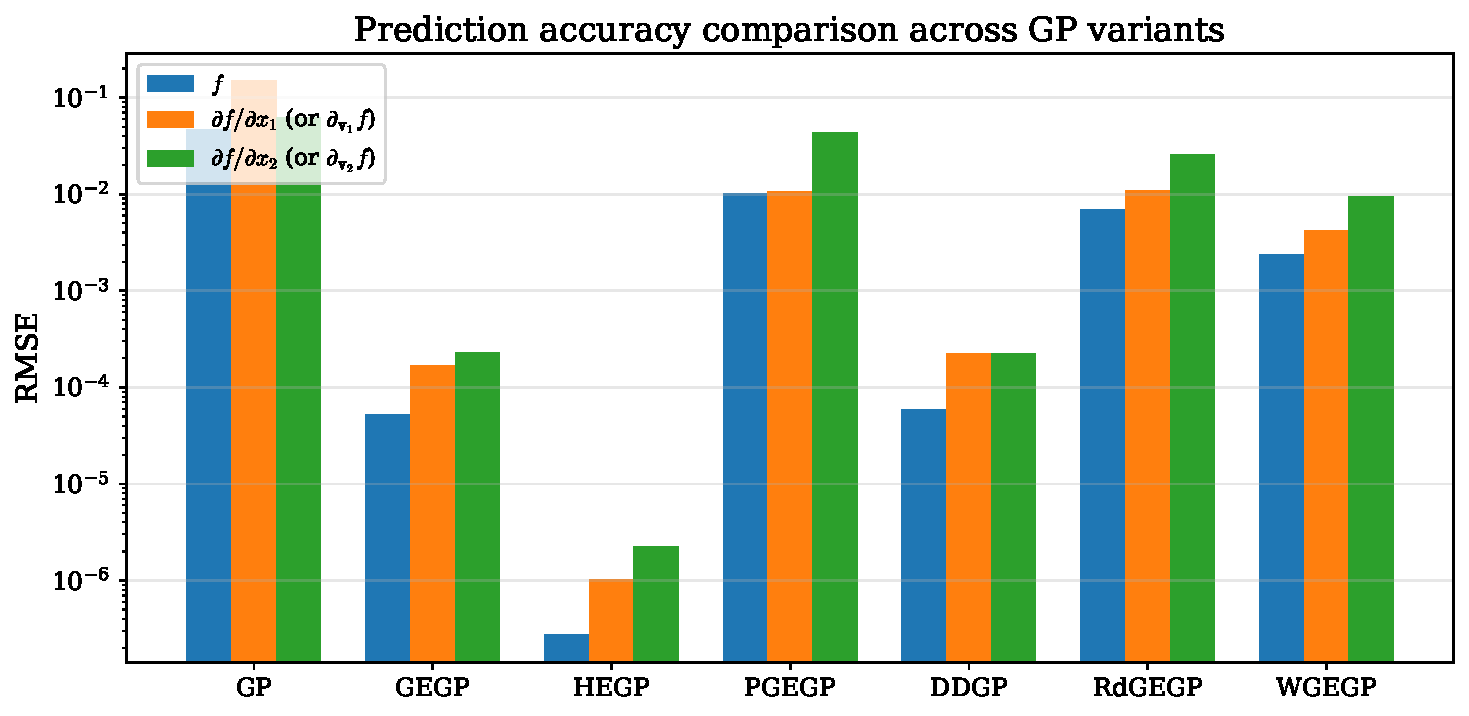
\includegraphics[width=\textwidth]{summary_rmse.pdf}
	\caption{RMSE comparison across GP variants on $f(x_1, x_2) = \sin(x_1)\cos(x_2)$ (log scale). The standard GP, trained on function values only, serves as a baseline. All derivative-enhanced methods substantially improve upon it, with the HEGP achieving the lowest error by several orders of magnitude.}
	\label{fig:summary_rmse}
\end{figure}

Several trends are evident from these results:

\begin{itemize}
	\item \textbf{Derivative information dramatically improves accuracy.} The standard GP, trained on function values alone, achieves an $f$ RMSE of $4.72 \times 10^{-2}$. While derivative predictions are available from the posterior cross-covariance, they exhibit high error ($1.49 \times 10^{-1}$ for $\partial f / \partial x_1$). Adding first-order gradient observations (GEGP) reduces the function RMSE by three orders of magnitude and yields derivative RMSE below $10^{-4}$.

	\item \textbf{Higher-order derivatives provide further gains.} The HEGP, which includes gradient and Hessian information, achieves RMSE values three orders of magnitude lower than the GEGP, demonstrating the value of curvature information.

	\item \textbf{Directional derivatives can match coordinate-aligned derivatives.} The DDGP achieves accuracy comparable to the GEGP despite using derivatives along non-coordinate directions, confirming that well-chosen directions can effectively capture the function's local geometry.

	\item \textbf{Partial derivative information still helps.} The PGEGP, RdGEGP, and WGEGP all achieve substantially lower error than the standard GP despite using only subsets of the available derivative information. The WGEGP, which uses all gradient data distributed across two submodels, outperforms the RdGEGP (gradients at 10 of 25 points) by a factor of three.

	\item \textbf{Weighted decomposition preserves quality.} The WGEGP closely approaches full GEGP accuracy while operating on smaller covariance matrices, illustrating the efficiency of the weighted submodel approach.
\end{itemize}

These background methods form the foundation for the arbitrary-order extensions presented in Section~\ref{sec:methods}. The DEGP generalizes the GEGP and HEGP to derivatives of any order $p$; the DDGP framework extends to arbitrary-order directional derivatives; and the WDEGP unifies weighted decomposition with arbitrary-order derivative enhancement.

%==============================================================================
\section{Methods}
\label{sec:methods}
%==============================================================================
Arbitrary order derivative-enhanced Gaussian Processes (DEGPs) extend standard GP models by 
incorporating derivative information to improve predictive accuracy and capture 
local behavior of nonlinear functions. Higher-order derivatives provide increasingly 
detailed information about local function curvature and behavior, enabling more 
accurate approximations with fewer training points—particularly critical for 
expensive simulations where each evaluation may require hours or days of computation. 
However, existing derivative-enhanced GP methods—including gradient-enhanced 
Gaussian processes (GEGPs), Hessian-enhanced GPs (HEGP), and weighted gradient-enhanced GP
(WGEGP)—have been limited to at most second-order derivatives. Moreover, while
the weighted framework provides a computationally efficient approach by decomposing
the problem into smaller submodels, the existing WGEGP methodology has only been applied
to first-order gradients, leaving unexplored the potential benefits of weighted 
decomposition for higher-order derivatives.

This work advances these methods to accommodate arbitrary-order derivative 
information through a unified framework comprising the \textit{Derivative-Enhanced 
	Gaussian Process (DEGP)}, the \textit{Directional Derivative Gaussian Process 
	(DDGP)}, and the \textit{Weighted Derivative-Enhanced Gaussian Process (WDEGP)}. These methods generalize existing gradient- and Hessian-enhanced GPs to arbitrary derivative order; when referring to prior first-order methods, we use the terms GEGP or WGEGP explicitly.

A key innovation of the proposed framework is the ability to specify derivative 
information flexibly at each training site. Rather than requiring uniform derivative 
specifications across all training points, the formulation permits independent 
selection of which derivatives to include—and at what order—for each location. 
Concretely, training point $\mathbf{x}_i$ might include derivatives up to order $p_i = 3$, 
while $\mathbf{x}_j$ includes only first-order derivatives ($p_j = 1$), and $\mathbf{x}_k$ 
includes no derivatives at all. For directional derivatives, both the number of 
directions $q_i$ and the derivative orders along each direction can vary by site. 
The formulations in the following sections assume uniform specifications across sites 
for notational simplicity, but all methods are implemented with full site-specific 
flexibility in JetGP, an open-source Python library accompanying this work that provides 
a unified implementation of the DEGP, DDGP, WDEGP, and WDDGP frameworks.\footnote{JetGP is available at \url{https://github.com/Samm-Py/jetgp}}

This site-specific flexibility enables adaptive derivative allocation strategies 
tailored to problem structure. For instance, in uncertainty quantification problems 
where inputs follow a probability distribution, higher-order derivatives can be 
concentrated at the distribution mean to maximize local accuracy where probability 
mass is highest, while lower-order derivatives at peripheral points provide broader 
coverage at reduced computational cost. Similarly, in optimization contexts, 
higher-order information near suspected optima can accelerate convergence while 
sparser derivative specifications suffice in exploratory regions.

The framework incorporates three complementary mechanisms for managing computational 
complexity. First, the \textit{Directional Derivative Gaussian Process (DDGP)} replaces the dimension-dependent partial derivative count with derivatives along a small number of selected directions, achieving dimension-independent complexity. Second, \textit{derivative screening} enables selective inclusion of 
specific derivative terms rather than requiring all derivatives up to a given order. 
Third, the \textit{Weighted Derivative-Enhanced Gaussian Process (WDEGP)}—extending WGEGP to arbitrary-order 
derivatives—decomposes the problem into submodels with heterogeneous derivative 
orders and specifications. Each submodel independently specifies which training 
points include derivatives, which derivative terms are incorporated, and at what 
orders, with predictions combined through weighted summation that preserves 
interpolation conditions.

%==============================================================================
\subsection{Arbitrary Order Derivative-Enhanced Gaussian Processes}
\label{subsec:degp}
%==============================================================================

The DEGP framework generalizes gradient/Hessian-enhanced GPs by including all partial derivatives up to a specified order $p$ at each training point. Given training inputs $\mathbf{X} = \{\mathbf{x}_i\}_{i=1}^{n}$ and corresponding function evaluations $f_i = f(\mathbf{x}_i)$, the augmented training set is defined as
\begin{equation}
	X^{(p)} := \left\{ \left( \mathbf{x}_i, \left( f_i, D^{\boldsymbol{\alpha}} f_i \right) \right), \; i = 1{:}n \right\},
\end{equation}
where $D^{\boldsymbol{\alpha}} f$ denotes the partial derivative operator for multi-index $\boldsymbol{\alpha} = (\alpha_1, \dots, \alpha_d)$ with $|\boldsymbol{\alpha}| = \alpha_1 + \cdots + \alpha_d \le p$:
\begin{equation}
	D^{\boldsymbol{\alpha}} f = \partial^{|\boldsymbol{\alpha}|}_{x_1^{\alpha_1} \cdots x_d^{\alpha_d}} f.
\end{equation}

As in Section~\ref{subsec:derivative_gps}, the observation vector $\mathbf{y}$ is expanded into an augmented vector $\mathbf{y}^{\boldsymbol{\alpha}}$, and the predictions at the test locations $\mathbf{X}_*$ are also augmented to include all such derivatives with $1 \leq |\boldsymbol{\alpha}| \leq p$, forming a vector $\mathbf{y}^{\boldsymbol{\alpha}}_*$:
\begin{equation}
	\label{eqn:degp_aug_vectors}
	\mathbf{y}^{\boldsymbol{\alpha}} = \begin{bmatrix} f(\mathbf{X}) \\ \{D^{\boldsymbol{\alpha}} f(\mathbf{X})\}_{1 \leq |\boldsymbol{\alpha}| \leq p} \end{bmatrix}, \quad
	\mathbf{y}^{\boldsymbol{\alpha}}_* = \begin{bmatrix} f(\mathbf{X}_*) \\ \{D^{\boldsymbol{\alpha}} f(\mathbf{X}_*)\}_{1 \leq |\boldsymbol{\alpha}| \leq p}\end{bmatrix}
\end{equation}
The joint distribution between the augmented training observations and the augmented test predictions is a multivariate Gaussian:
\begin{equation}
	\label{eqn:full_dek_joint_dist}
	\begin{pmatrix}
		\mathbf{y}^{\boldsymbol{\alpha}} \\
		\mathbf{y}^{\boldsymbol{\alpha}}_*
	\end{pmatrix}
	\sim \mathcal{N}\left(
	\mathbf{0},
	\begin{pmatrix}
		\boldsymbol{\Sigma}^{\boldsymbol{\alpha}}_{11} & \boldsymbol{\Sigma}^{\boldsymbol{\alpha}}_{12} \\
		\boldsymbol{\Sigma}^{\boldsymbol{\alpha}}_{21} & \boldsymbol{\Sigma}^{\boldsymbol{\alpha}}_{22}
	\end{pmatrix}
	\right),
\end{equation}
where the training covariance block, $\boldsymbol{\Sigma}^{\boldsymbol{\alpha}}_{11}$, is an $n\binom{d + p}{p} \times n\binom{d + p}{p}$ matrix:
\begin{equation}
	\label{eqn:full_dek_S11}
	\boldsymbol{\Sigma}^{\boldsymbol{\alpha}}_{11} =
	\begin{pmatrix} 
		K_{\boldsymbol{\alpha}^{(0)}\boldsymbol{\alpha}^{(0)}} & K_{\boldsymbol{\alpha}^{(0)}\boldsymbol{\alpha}^{(1)}} & \cdots & K_{\boldsymbol{\alpha}^{(0)}\boldsymbol{\alpha}^{(M)}} \\ 
		K_{\boldsymbol{\alpha}^{(1)}\boldsymbol{\alpha}^{(0)}} & K_{\boldsymbol{\alpha}^{(1)}\boldsymbol{\alpha}^{(1)}} & \cdots & K_{\boldsymbol{\alpha}^{(1)}\boldsymbol{\alpha}^{(M)}} \\ 
		\vdots & \vdots & \ddots & \vdots \\ 
		K_{\boldsymbol{\alpha}^{(M)}\boldsymbol{\alpha}^{(0)}} & K_{\boldsymbol{\alpha}^{(M)}\boldsymbol{\alpha}^{(1)}} & \cdots & K_{\boldsymbol{\alpha}^{(M)}\boldsymbol{\alpha}^{(M)}} 
	\end{pmatrix}
\end{equation}
where $M = \binom{d+p}{p} - 1$ is the total number of derivative terms, and $\{\boldsymbol{\alpha}^{(0)}, \boldsymbol{\alpha}^{(1)}, \ldots, \boldsymbol{\alpha}^{(M)}\}$ enumerates all multi-indices with $|\boldsymbol{\alpha}^{(i)}| \leq p$, ordered such that $\boldsymbol{\alpha}^{(0)} = (0,\ldots,0)$ corresponds to the function value. Each block $K_{\boldsymbol{\beta}\boldsymbol{\gamma}}$ is an $n \times n$ matrix with entries:
\begin{equation}
	[K_{\boldsymbol{\beta}\boldsymbol{\gamma}}]_{ij} = D_{\mathbf{x}_i}^{\boldsymbol{\beta}} D_{\mathbf{x}_j'}^{\boldsymbol{\gamma}} k(\mathbf{x}_i, \mathbf{x}_j) = \partial^{|\boldsymbol{\beta}| + |\boldsymbol{\gamma}|}_{\mathbf{x}_i^{\boldsymbol{\beta}}\,\mathbf{x}_j^{\boldsymbol{\gamma}}} k(\mathbf{x}_i, \mathbf{x}_j).
\end{equation}
The training-test block $\boldsymbol{\Sigma}^{\boldsymbol{\alpha}}_{12}$ and test-test block $\boldsymbol{\Sigma}^{\boldsymbol{\alpha}}_{22}$ are constructed analogously. The posterior predictive distribution for the augmented test vector $\mathbf{y}^{\boldsymbol{\alpha}}_*$ is given by:
\begin{equation}
	\label{eqn:full_dek_posterior}
	\begin{split}
		\boldsymbol{\mu}_{*} &= \boldsymbol{\Sigma}^{\boldsymbol{\alpha}}_{21} \left(\boldsymbol{\Sigma}^{\boldsymbol{\alpha}}_{11}\right)^{-1} \mathbf{y}^{\boldsymbol{\alpha}} \\
		\boldsymbol{\Sigma}_{*} &=  \boldsymbol{\Sigma}^{\boldsymbol{\alpha}}_{22} - \boldsymbol{\Sigma}^{\boldsymbol{\alpha}}_{21} \left(\boldsymbol{\Sigma}^{\boldsymbol{\alpha}}_{11}\right)^{-1} \boldsymbol{\Sigma}^{\boldsymbol{\alpha}}_{12}
	\end{split}
\end{equation}
The kernel hyperparameters $\boldsymbol{\psi}$ are determined by maximizing the log marginal likelihood (MLL) of the augmented observations:
\begin{equation}
	\label{eqn:dek_mll}
	\log p(\mathbf{y}^{\boldsymbol{\alpha}}|\mathbf{X}, \boldsymbol{\psi}) = -\frac{1}{2} \left(\mathbf{y}^{\boldsymbol{\alpha}}\right)^\top \left(\boldsymbol{\Sigma}^{\boldsymbol{\alpha}}_{11}\right)^{-1} \mathbf{y}^{\boldsymbol{\alpha}} - \frac{1}{2}\log|\boldsymbol{\Sigma}^{\boldsymbol{\alpha}}_{11}| - C
\end{equation}
where $C > 0$ is a constant term. When incorporating higher-order derivatives, the size of the matrix $\boldsymbol{\Sigma}^{\boldsymbol{\alpha}}_{11}$ grows rapidly with both the number of training points $n$ and the dimensionality $d$. Specifically, the cost of Cholesky decomposition scales as $\mathcal{O}\left(\left(n \binom{d + p}{p}\right)^3\right)$, which quickly becomes prohibitive. This computational challenge is addressed through three complementary strategies: directional derivatives (Section~\ref{subsec:ddgp}), which replace the dimension-dependent $\binom{d+p}{p}$ term with $\binom{q+p}{q}$ for $q \ll d$ selected directions; derivative screening (Section~\ref{subsec:derivative_screening}), where at each training site only the most informative derivative terms are included; and weighted decomposition (Section~\ref{subsec:wdegp}), which partitions the problem into smaller submodels.
%==============================================================================
\subsection{Arbitrary Order Directional Derivative Gaussian Process}
\label{subsec:ddgp}
%==============================================================================

The DDGP extends the directional derivative GP framework (Section~\ref{subsec:ddgp}) to arbitrary-order derivatives. Rather than including all $\binom{d+p}{p}$ partial derivatives, DDGP uses derivatives along $q$ selected directions.

For each training point $\mathbf{x}_i$, let $\mathbf{V}_i = \{\mathbf{v}_{i,1}, \ldots, \mathbf{v}_{i,q}\}$ denote $q$ unit direction vectors ($\|\mathbf{v}_{i,j}\| = 1$). The directional derivative of order $r$ along direction $\mathbf{v}$ is:
\begin{equation}
	\partial^r_{\mathbf{v}^r} f(\mathbf{x}) = \left.\frac{d^r}{dt^r} f(\mathbf{x} + t\mathbf{v})\right|_{t=0}.
\end{equation}

Using multi-index notation for the $q$ directions, let $\boldsymbol{\beta} = (\beta_1, \ldots, \beta_q)$ where $\beta_j$ denotes the derivative order along direction $\mathbf{v}_j$. The mixed directional derivative is:
\begin{equation}
	D_{\mathbf{V}}^{\boldsymbol{\beta}} f(\mathbf{x}) = \partial^{|\boldsymbol{\beta}|}_{\mathbf{v}_1^{\beta_1} \cdots \mathbf{v}_q^{\beta_q}} f(\mathbf{x}),
\end{equation}
where $|\boldsymbol{\beta}| = \sum_{j=1}^q \beta_j \leq p$.

The augmented training vector includes all directional derivative terms up to total order $p$:
\begin{equation}
	\label{eqn:ddgp_aug_vector}
	\mathbf{y}_{DD}^{(p)} = 
	\begin{bmatrix} 
		f(\mathbf{X}) \\
		\{D_{\mathbf{V}_i}^{\boldsymbol{\beta}} f(\mathbf{x}_i)\}_{|\boldsymbol{\beta}| \leq p, \, i=1,\ldots,n}
	\end{bmatrix} \in \mathbb{R}^{n\binom{q+p}{q}},
\end{equation}
where the set $\{\boldsymbol{\beta} : |\boldsymbol{\beta}| \leq p\}$ contains $\binom{q+p}{q}$ multi-indices. For test points $\mathbf{X}_*$ with directions $\mathbf{V}_*$, the test vector $\mathbf{y}_{DD,*}^{(p)}$ is defined analogously.

The joint distribution of training and test observations is:
\begin{equation}
	\label{eqn:ddgp_joint}
	\begin{pmatrix} 
		\mathbf{y}_{DD}^{(p)} \\ 
		\mathbf{y}_{DD,*}^{(p)} 
	\end{pmatrix} \sim 
	\mathcal{N}\left( 
	\mathbf{0}, 
	\begin{pmatrix} 
		\boldsymbol{\Sigma}_{11}^{DD} & \boldsymbol{\Sigma}_{12}^{DD} \\ 
		\boldsymbol{\Sigma}_{21}^{DD} & \boldsymbol{\Sigma}_{22}^{DD} 
	\end{pmatrix} 
	\right).
\end{equation}

The training covariance block $\boldsymbol{\Sigma}_{11}^{DD}$ is an $n\binom{q+p}{q} \times n\binom{q+p}{q}$ matrix. Let $\mathcal{B}_p^q = \{\boldsymbol{\beta} \in \mathbb{N}_0^q : |\boldsymbol{\beta}| \leq p\}$ denote the set of directional multi-indices, and enumerate them as $\{\boldsymbol{\beta}^{(0)}, \boldsymbol{\beta}^{(1)}, \ldots, \boldsymbol{\beta}^{(N_p^q-1)}\}$ where $N_p^q = \binom{q+p}{q}$ and $\boldsymbol{\beta}^{(0)} = (0,\ldots,0)$. The covariance matrix has block structure:
\begin{equation}
	\label{eqn:ddgp_S11}
	\boldsymbol{\Sigma}_{11}^{DD} =
	\begin{pmatrix} 
		K_{\boldsymbol{\beta}^{(0)}\boldsymbol{\beta}^{(0)}} & K_{\boldsymbol{\beta}^{(0)}\boldsymbol{\beta}^{(1)}} & \cdots & K_{\boldsymbol{\beta}^{(0)}\boldsymbol{\beta}^{(N_p^q-1)}} \\ 
		K_{\boldsymbol{\beta}^{(1)}\boldsymbol{\beta}^{(0)}} & K_{\boldsymbol{\beta}^{(1)}\boldsymbol{\beta}^{(1)}} & \cdots & K_{\boldsymbol{\beta}^{(1)}\boldsymbol{\beta}^{(N_p^q-1)}} \\ 
		\vdots & \vdots & \ddots & \vdots \\ 
		K_{\boldsymbol{\beta}^{(N_p^q-1)}\boldsymbol{\beta}^{(0)}} & K_{\boldsymbol{\beta}^{(N_p^q-1)}\boldsymbol{\beta}^{(1)}} & \cdots & K_{\boldsymbol{\beta}^{(N_p^q-1)}\boldsymbol{\beta}^{(N_p^q-1)}} 
	\end{pmatrix},
\end{equation}
where each block $K_{\boldsymbol{\beta}\boldsymbol{\gamma}}$ is an $n \times n$ matrix with entries:
\begin{equation}
	[K_{\boldsymbol{\beta}\boldsymbol{\gamma}}]_{ij} = D_{\mathbf{V}_i}^{\boldsymbol{\beta}} D_{\mathbf{V}_j}^{\boldsymbol{\gamma}} k(\mathbf{x}_i, \mathbf{x}_j),
\end{equation}
representing the covariance between the $\boldsymbol{\beta}$-directional derivative at $\mathbf{x}_i$ and the $\boldsymbol{\gamma}$-directional derivative at $\mathbf{x}_j$.

The training-test and test-test covariance blocks $\boldsymbol{\Sigma}_{12}^{DD}$ and $\boldsymbol{\Sigma}_{22}^{DD}$ are constructed analogously. The posterior predictive distribution follows the standard GP formula:
\begin{equation}
	\label{eqn:ddgp_posterior}
	\begin{aligned}
		\boldsymbol{\mu}_{*} &= \boldsymbol{\Sigma}_{21}^{DD} \left(\boldsymbol{\Sigma}_{11}^{DD}\right)^{-1} \mathbf{y}_{DD}^{(p)}, \\
		\boldsymbol{\Sigma}_{*} &= \boldsymbol{\Sigma}_{22}^{DD} - \boldsymbol{\Sigma}_{21}^{DD} \left(\boldsymbol{\Sigma}_{11}^{DD}\right)^{-1} \boldsymbol{\Sigma}_{12}^{DD},
	\end{aligned}
\end{equation}
where $\boldsymbol{\mu}_*$ is the predictive mean and $\boldsymbol{\Sigma}_*$ is the predictive covariance.

Kernel hyperparameters are optimized by maximizing the log marginal likelihood:
\begin{equation}
	\label{eqn:ddgp_mll}
	\log p(\mathbf{y}_{DD}^{(p)}|\mathbf{X}, \mathbf{V}, \boldsymbol{\psi}) = -\frac{1}{2} \left(\mathbf{y}_{DD}^{(p)}\right)^\top \left(\boldsymbol{\Sigma}_{11}^{DD}\right)^{-1} \mathbf{y}_{DD}^{(p)} - \frac{1}{2}\log|\boldsymbol{\Sigma}_{11}^{DD}| - C,
\end{equation}
where $C$ is a constant term.

The computational cost is:
\begin{equation}
	\mathcal{O}\left(\left(n\binom{q+p}{q}\right)^3\right),
\end{equation}
which is independent of the ambient dimension $d$. For example, with $q=3$, $p=3$, and $n=100$, the matrix size is $2{,}000 \times 2{,}000$ regardless of whether $d=10$ or $d=1000$. This dimension-independence makes DDGP particularly attractive for high-dimensional problems where DEGP becomes intractable.

As with DEGP, the number of derivative terms can be further reduced through screening strategies that select subsets of directional derivative multi-indices; this extension is developed in Section~\ref{subsec:derivative_screening}.

%==============================================================================
\subsection{Derivative Screening Strategies}
\label{subsec:derivative_screening}
%==============================================================================

The computational burden of both DEGP and DDGP grows rapidly with derivative order, as the number of terms scales combinatorially. Derivative screening addresses this by selectively including only the most informative derivative terms rather than the complete derivative tensor. This extends the PGEGP concept (Section~\ref{subsec:pgegp}) to arbitrary-order settings for both partial and directional derivatives.

While the formulations below assume uniform screening across sites for notational simplicity, the framework naturally extends to site-specific derivative allocation, where each training point can have its own selected subset. This flexibility enables adaptive strategies such as concentrating higher-order derivatives at locations of greatest interest (e.g., the mean of an input distribution in UQ applications) while using lower-order derivatives elsewhere. Site-specific screening for both variants is implemented in JetGP.

\subsubsection{Screening for Partial Derivatives}
\label{subsubsec:partial_screening}

Let $\mathcal{A}_p = \{\boldsymbol{\alpha} \in \mathbb{N}_0^d : |\boldsymbol{\alpha}| \leq p\}$ denote the complete set of multi-indices up to order $p$, containing $\binom{d+p}{p}$ elements. Screening identifies a subset $\mathcal{A}_{\text{sel}} \subset \mathcal{A}_p$ of size $|\mathcal{A}_{\text{sel}}| = M_{\text{sel}} \ll \binom{d+p}{p}$ containing the most informative terms.

Given the selected subset $\mathcal{A}_{\text{sel}} = \{\boldsymbol{\alpha}^{(1)}, \ldots, \boldsymbol{\alpha}^{(M_{\text{sel}})}\}$, the augmented observation vectors include only these derivatives:
\begin{equation}
	\label{eqn:screened_aug_vectors}
	\mathbf{y}^{\text{scr}} = \begin{bmatrix} 
		f(\mathbf{X}) \\ 
		D^{\boldsymbol{\alpha}^{(1)}} f(\mathbf{X}) \\ 
		\vdots \\ 
		D^{\boldsymbol{\alpha}^{(M_{\text{sel}})}} f(\mathbf{X})
	\end{bmatrix}, \quad
	\mathbf{y}^{\text{scr}}_* = \begin{bmatrix} 
		f(\mathbf{X}_*) \\ 
		D^{\boldsymbol{\alpha}^{(1)}} f(\mathbf{X}_*) \\ 
		\vdots \\ 
		D^{\boldsymbol{\alpha}^{(M_{\text{sel}})}} f(\mathbf{X}_*)
	\end{bmatrix}.
\end{equation}

The joint distribution follows the standard GP structure:
\begin{equation}
	\label{eqn:screened_joint_dist}
	\begin{pmatrix}
		\mathbf{y}^{\text{scr}} \\
		\mathbf{y}^{\text{scr}}_*
	\end{pmatrix}
	\sim \mathcal{N}\left(
	\mathbf{0},
	\begin{pmatrix}
		\boldsymbol{\Sigma}^{\text{scr}}_{11} & \boldsymbol{\Sigma}^{\text{scr}}_{12} \\
		\boldsymbol{\Sigma}^{\text{scr}}_{21} & \boldsymbol{\Sigma}^{\text{scr}}_{22}
	\end{pmatrix}
	\right),
\end{equation}
where the training covariance block $\boldsymbol{\Sigma}^{\text{scr}}_{11}$ is an $n(M_{\text{sel}} + 1) \times n(M_{\text{sel}} + 1)$ matrix with the same block structure as Equation~\eqref{eqn:full_dek_S11}, but restricted to the selected multi-indices:
\begin{equation}
	\label{eqn:screened_S11}
	\boldsymbol{\Sigma}^{\text{scr}}_{11} =
	\begin{pmatrix} 
		K_{\boldsymbol{\alpha}^{(0)}\boldsymbol{\alpha}^{(0)}} & K_{\boldsymbol{\alpha}^{(0)}\boldsymbol{\alpha}^{(1)}} & \cdots & K_{\boldsymbol{\alpha}^{(0)}\boldsymbol{\alpha}^{(M_{\text{sel}})}} \\ 
		K_{\boldsymbol{\alpha}^{(1)}\boldsymbol{\alpha}^{(0)}} & K_{\boldsymbol{\alpha}^{(1)}\boldsymbol{\alpha}^{(1)}} & \cdots & K_{\boldsymbol{\alpha}^{(1)}\boldsymbol{\alpha}^{(M_{\text{sel}})}} \\ 
		\vdots & \vdots & \ddots & \vdots \\ 
		K_{\boldsymbol{\alpha}^{(M_{\text{sel}})}\boldsymbol{\alpha}^{(0)}} & K_{\boldsymbol{\alpha}^{(M_{\text{sel}})}\boldsymbol{\alpha}^{(1)}} & \cdots & K_{\boldsymbol{\alpha}^{(M_{\text{sel}})}\boldsymbol{\alpha}^{(M_{\text{sel}})}} 
	\end{pmatrix}.
\end{equation}
The training-test and test-test blocks are constructed analogously. Posterior prediction and hyperparameter optimization follow Equations~\eqref{eqn:full_dek_posterior} and~\eqref{eqn:dek_mll} with the screened covariance matrices.

The Cholesky decomposition cost reduces from $\mathcal{O}((n\binom{d+p}{p})^3)$ to $\mathcal{O}((n(M_{\text{sel}} + 1))^3)$. For example, with $d=10$, $p=3$, and $n=100$, the full matrix has dimension $28{,}600 \times 28{,}600$, requiring approximately $2.3 \times 10^{13}$ operations. Screening to $M_{\text{sel}} = 50$ derivatives reduces the matrix to $5{,}100 \times 5{,}100$, requiring $1.3 \times 10^{11}$ operations---a reduction of over 99\%.

\subsubsection{Screening for Directional Derivatives}
\label{subsubsec:directional_screening}

The screening framework extends directly to directional derivatives. Let $\mathcal{B}_p^q = \{\boldsymbol{\beta} \in \mathbb{N}_0^q : |\boldsymbol{\beta}| \leq p\}$ denote the complete set of directional multi-indices. Screening identifies a subset $\mathcal{B}_{\text{sel}} \subset \mathcal{B}_p^q$ of size $|\mathcal{B}_{\text{sel}}| = L_{\text{sel}} \ll \binom{q+p}{q}$.

The screened augmented observation vector is:
\begin{equation}
	\label{eqn:screened_dd_aug_vector}
	\mathbf{y}_{DD}^{\text{scr}} = 
	\begin{bmatrix} 
		f(\mathbf{X}) \\
		\{D_{\mathbf{V}_i}^{\boldsymbol{\beta}} f(\mathbf{x}_i)\}_{\boldsymbol{\beta} \in \mathcal{B}_{\text{sel}}, \, i=1,\ldots,n}
	\end{bmatrix} \in \mathbb{R}^{n(L_{\text{sel}} + 1)}.
\end{equation}

The covariance structure parallels Equation~\eqref{eqn:screened_S11}, with directional derivative kernels $D_{\mathbf{V}_i}^{\boldsymbol{\beta}} D_{\mathbf{V}_j}^{\boldsymbol{\gamma}} k(\mathbf{x}_i, \mathbf{x}_j)$ replacing partial derivative kernels. The computational complexity reduces to $\mathcal{O}((n(L_{\text{sel}} + 1))^3)$, independent of both ambient dimension $d$ and the full directional term count $\binom{q+p}{q}$.

The optimal screening strategy depends on problem structure and computational budget; selection criteria are discussed in Section~\ref{sec:discussion}. JetGP supports arbitrary user-specified subsets $\mathcal{A}_{\text{sel}}$ or $\mathcal{B}_{\text{sel}}$, enabling application-specific screening criteria.

%==============================================================================
\subsection{Weighted Arbitrary Order Derivative-Enhanced Gaussian Process}
\label{subsec:wdegp}
%==============================================================================

The WGEGP framework (Section~\ref{subsec:derivative_gps}) provides computational efficiency by decomposing derivative-enhanced GPs into smaller submodels, but is limited to first-order gradients. This section extends the weighted framework to arbitrary-order derivatives while incorporating the screening strategies from Sections~\ref{subsubsec:partial_screening} and~\ref{subsubsec:directional_screening}.

The extension admits two variants depending on derivative representation:
\begin{itemize}
	\item \textbf{WDEGP}: Submodels use partial derivatives with screening as in Section~\ref{subsubsec:partial_screening}
	\item \textbf{WDDGP}: Submodels use directional derivatives with screening as in Section~\ref{subsubsec:directional_screening}
\end{itemize}

Given a training dataset $\mathcal{D}$ with $n$ input-output pairs and derivative information, each submodel $k \in \{1, \ldots, M\}$ independently specifies:
\begin{itemize}
	\item $\mathcal{I}_k \subseteq \{1, \ldots, n\}$: training point indices where derivatives are included
	\item For WDEGP: $\mathcal{A}_k \subseteq \mathcal{A}_{p_{\max}}$, the selected partial derivative multi-indices
	\item For WDDGP: $\mathcal{B}_k \subseteq \mathcal{B}_{p_k}^{q_k}$, the selected directional derivative multi-indices, with direction vectors $\mathbf{V}_k = \{\mathbf{V}_{k,i}\}_{i \in \mathcal{I}_k}$
\end{itemize}

The total number of derivative observations in submodel $k$ is:
\begin{equation}
	N_k^{\text{deriv}} = \begin{cases}
		|\mathcal{A}_k| \cdot |\mathcal{I}_k| & \text{for WDEGP}, \\
		|\mathcal{B}_k| \cdot |\mathcal{I}_k| & \text{for WDDGP},
	\end{cases}
\end{equation}
generalizing the $d|\mathcal{I}_k|$ gradient observations in WGEGP. The augmented observation vector for submodel $k$ is:
\begin{equation}
	\label{eqn:wdegp_aug_vector}
	\mathbf{y}^{(k)} = \begin{bmatrix} 
		f(\mathbf{X}) \\
		\{D^{\boldsymbol{\alpha}} f(\mathbf{x}_i)\}_{\boldsymbol{\alpha} \in \mathcal{A}_k, i \in \mathcal{I}_k}
	\end{bmatrix} \in \mathbb{R}^{n + N_k^{\text{deriv}}},
\end{equation}
for WDEGP, with the analogous directional derivative formulation for WDDGP.

The training covariance block $\boldsymbol{\Sigma}^{(k)}_{11} \in \mathbb{R}^{(n + N_k^{\text{deriv}}) \times (n + N_k^{\text{deriv}})}$ retains the structure of Equation~\eqref{eqn:wgek_S11}:
\begin{equation}
	\label{eqn:wdegp_S11}
	\boldsymbol{\Sigma}^{(k)}_{11} =
	\begin{pmatrix}
		\mathbf{K}_{ff} & \mathbf{K}_{fd}^{(k)} \\
		\left(\mathbf{K}_{fd}^{(k)}\right)^\top & \mathbf{K}_{dd}^{(k)}
	\end{pmatrix},
\end{equation}
where $\mathbf{K}_{ff} = K(\mathbf{X}, \mathbf{X}) \in \mathbb{R}^{n \times n}$, $\mathbf{K}_{fd}^{(k)} \in \mathbb{R}^{n \times N_k^{\text{deriv}}}$, and $\mathbf{K}_{dd}^{(k)} \in \mathbb{R}^{N_k^{\text{deriv}} \times N_k^{\text{deriv}}}$. The entries of $\mathbf{K}_{fd}^{(k)}$ and $\mathbf{K}_{dd}^{(k)}$ are computed using the derivative kernels $D_{\mathbf{x}}^{\boldsymbol{\alpha}} D_{\mathbf{x}'}^{\boldsymbol{\gamma}} k(\mathbf{x}, \mathbf{x}')$ for WDEGP or $D_{\mathbf{V}}^{\boldsymbol{\beta}} D_{\mathbf{V}'}^{\boldsymbol{\gamma}} k(\mathbf{x}, \mathbf{x}')$ for WDDGP, as defined in the respective sections. The cross-covariance and test covariance blocks follow analogously.

Posterior prediction, weight computation, and hyperparameter optimization proceed exactly as in WGEGP. Submodel predictions are computed via Equation~\eqref{eqn:wgek_posterior} and combined through the weighted sum in Equation~\eqref{eqn:wgek_weighted_prediction}, with weights satisfying Equation~\eqref{eqn:wgek_weight_constraints} and computed via Equations~\eqref{eqn:wgek_weight_system}--\eqref{eqn:wgek_submodel_weights}. Shared hyperparameters are optimized by maximizing the joint log-likelihood in Equation~\eqref{eqn:wgek_jll}.

The computational complexity is:
\begin{equation}
	\mathcal{O}\left(\sum_{k=1}^M (n + N_k^{\text{deriv}})^3\right),
\end{equation}
compared to $\mathcal{O}((n\binom{d+p}{p})^3)$ for full DEGP. The reduction arises from spatial partitioning (smaller $|\mathcal{I}_k|$) and derivative screening (smaller $|\mathcal{A}_k|$ or $|\mathcal{B}_k|$). For WDDGP, complexity depends on the number of directions $q_k$ rather than the ambient dimension $d$, providing an additional reduction in high-dimensional settings. The choice of $M$ and partitioning strategy represents a trade-off between computational efficiency and model accuracy, as discussed in Section~\ref{subsec:derivative_gps}. Both variants are implemented in JetGP.

	\section{Results}
	\label{sec:experiments}
	%==============================================================================
	
	\todo{Add numerical experiments comparing:
		\begin{itemize}
			\item AO-DEGP vs GEK vs standard GP on test functions
			\item Effect of derivative order $p$ on accuracy
			\item Screening strategies and their accuracy-cost tradeoffs
			\item AO-DDGP dimension independence demonstration
			\item AO-WDEGP computational savings
			\item High-dimensional examples ($d \geq 10$)
		\end{itemize}
	}
	
	\subsection{Test Functions}
	\label{subsec:test_functions}
	
	We consider the following benchmark functions:
	
	\begin{enumerate}
		\item \textbf{Gramacy-Lee (1D)}: $f(x) = \frac{\sin(10\pi x)}{2x} + (x-1)^4$, $x \in [0.5, 2.5]$
		\item \textbf{Six-Hump Camel (2D)}: Multimodal function with six local minima
		\item \textbf{Rastrigin (scalable)}: Highly nonlinear with many local optima
		\item \textbf{Sum of Squares (scalable)}: $f(\x) = \sum_{i=1}^{d} i x_i^2$ for testing high-dimensional behavior
	\end{enumerate}
	
	\subsection{Accuracy vs. Derivative Order}
	\label{subsec:exp_order}
	
	\todo{Present RMSE and maximum error results showing benefit of higher-order derivatives}
	
	\subsection{Computational Scaling}
	\label{subsec:exp_scaling}
	
	\todo{Present timing results demonstrating computational complexity predictions}
	
	\subsection{High-Dimensional Examples}
	\label{subsec:exp_highdim}
	
	\todo{Demonstrate AO-DDGP on problems with $d \geq 10$}
	
	%==============================================================================
	\section{Discussion}
	

\section{Conclusions}
\label{sec:conclusions}

We have presented a unified framework for arbitrary-order derivative-enhanced Gaussian Processes that addresses fundamental limitations of existing methods. The framework comprises three complementary strategies for managing computational complexity:

\begin{enumerate}
	\item \textbf{DEGP} extends derivative enhancement to arbitrary order $p$ with flexible derivative screening strategies that selectively include only the most informative derivative terms.
	
	\item \textbf{DDGP} achieves dimension-independent complexity through directional derivatives along $q \ll d$ directions, replacing the $\binom{d+p}{p}$ partial derivative terms with $\binom{q+p}{q}$ directional terms.
	
	\item \textbf{WDEGP} extends weighted decomposition to arbitrary order with heterogeneous submodels, each specifying its own derivative terms and training point assignments.
\end{enumerate}

These strategies can be combined: WDDGP integrates directional derivatives with weighted decomposition, providing maximum flexibility for high-dimensional problems with limited computational budgets.

A key innovation of the framework is site-specific derivative allocation, where each training point can independently specify which derivatives to include and at what order. This enables adaptive strategies that concentrate higher-order information where it provides the greatest benefit.

The mathematical derivations establish the covariance structure for each formulation, and computational complexity analysis quantifies the tradeoffs between accuracy and cost. Numerical experiments demonstrate that higher-order derivatives can significantly improve surrogate accuracy, while directional and weighted strategies make these improvements computationally tractable for high-dimensional problems.

All methods are implemented in JetGP, an open-source Python library accompanying this work.

\todo{Add discussion of:
	\begin{itemize}
		\item Limitations and when each method is most appropriate
		\item Guidance for practitioners on method selection
		\item Future directions (adaptive methods, multi-fidelity, etc.)
	\end{itemize}
}

	
	%==============================================================================
	% References
	%==============================================================================
	\bibliographystyle{unsrt}
	\bibliography{gp_th}
	
\end{document}